% Changing book to article will make the footers match on each page,
% rather than alternate every other.
%
% Note that the article class does not have chapters.
\documentclass[letterpaper,10pt,twoside,openany]{book}

% Use babel or polyglossia to automatically redefine macros for terms
% Armor Class, Level, etc...
% Default output is in English; captions are located in lib/dndstring-captions.sty.
% If no captions exist for a language, English will be used.
%1. To load a language with babel:
%	\usepackage[<lang>]{babel}
%2. To load a language with polyglossia:
%	\usepackage{polyglossia}
%	\setdefaultlanguage{<lang>}
\usepackage[english]{babel}
%usepackage[italian]{babel}
% For further options (multilanguage documents, hypenations, language environments...)
% please refer to babel/polyglossia's documentation.

%\usepackage[utf8]{inputenc} %incompatible with fontspec
\usepackage{hang}
\usepackage{lipsum}
\usepackage{listings}
\usepackage{hyperref}
\usepackage{multicol}
\usepackage{fontspec}
\usepackage{dnd}

\lstset{%
  basicstyle=\ttfamily,
  language=[LaTeX]{TeX},
}

%Set's subsubsections to be included in the toc.
\setcounter{tocdepth}{3}

\usepackage{eso-pic}

\newcommand\BackgroundPicAlt{%
	\put(0,0){%
		\parbox[b][\paperheight]{\paperwidth}{%
			\vfill\underline{}
			\centering
			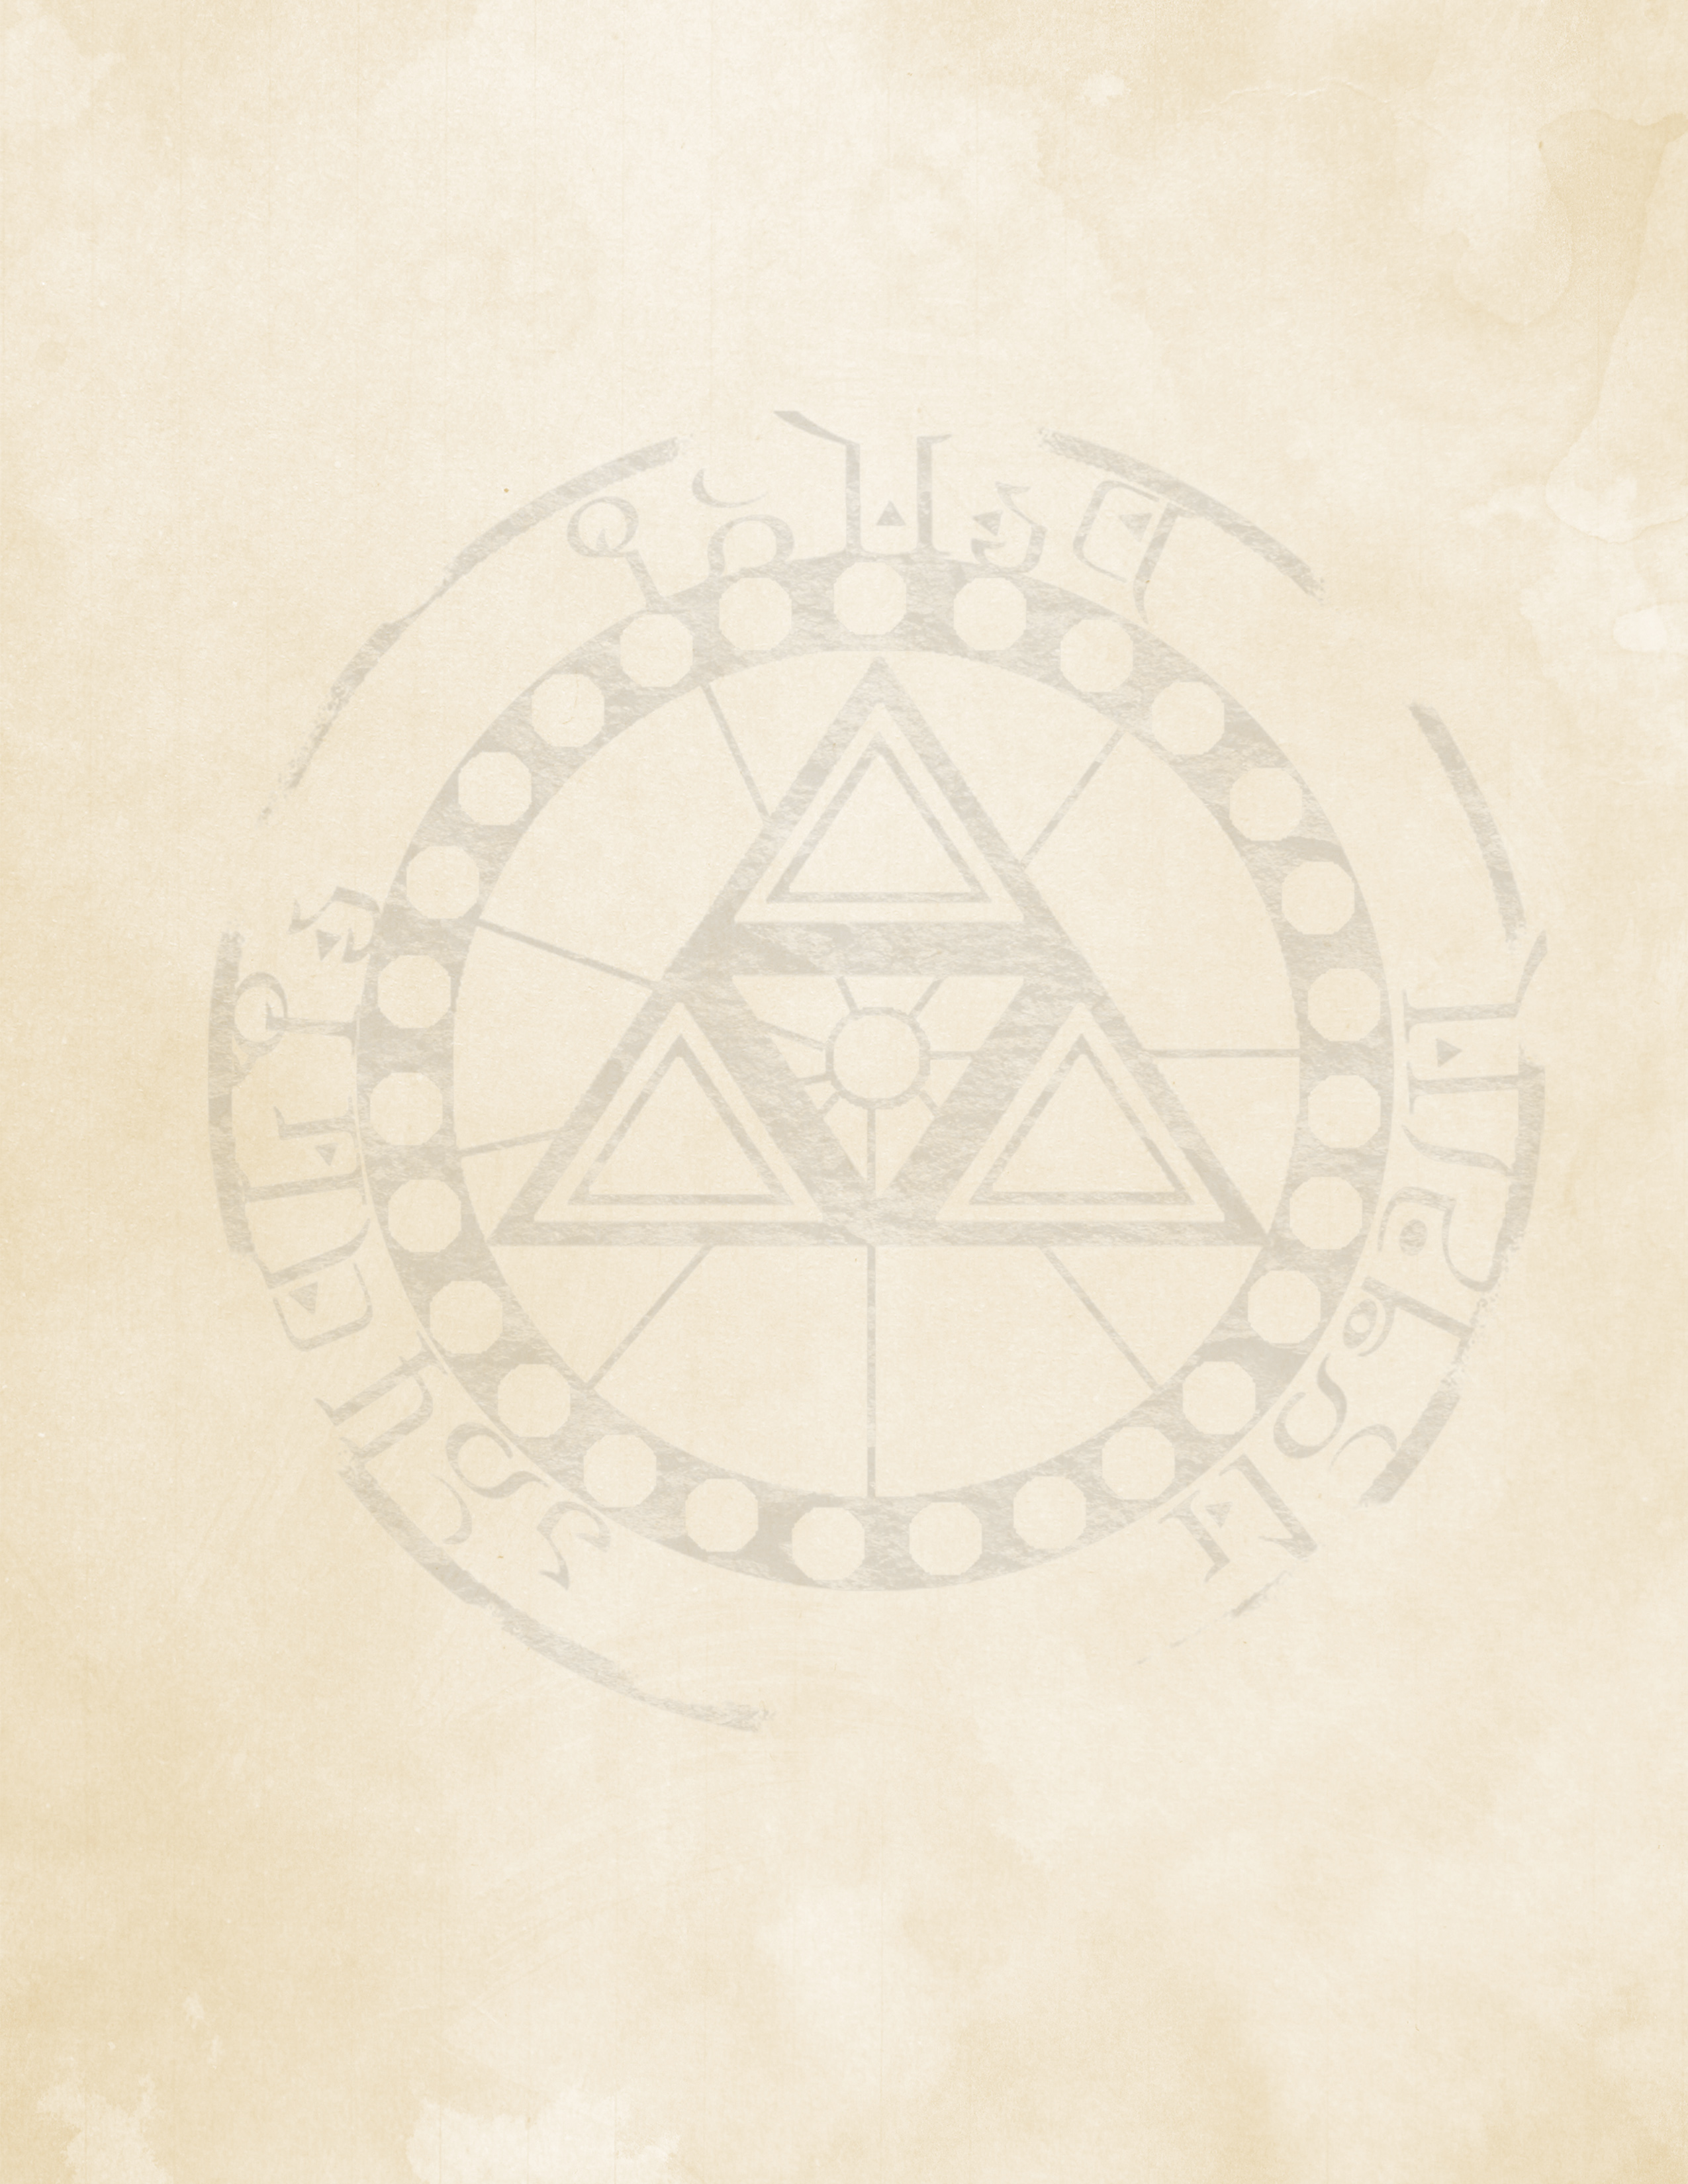
\includegraphics[width=\paperwidth,height=\paperheight,%
			keepaspectratio]{img/trinitypaper2.jpg} %Set to TrinityPaper1.jpg for printing
			\vfill
}}}

\title{The Enigma of the Trinity Stones}
\author{Antonius Torode}
\date{Latest update: \today}


% Start document
\begin{document}

\AddToShipoutPicture*{\BackgroundPicAlt}
\maketitle
\tableofcontents

\chapter{The Trinity Stones: History}

\begin{center}
	\includegraphics[width=\linewidth]{img/TS.jpg}
\end{center}


\section{Creation of a Trinity}

\begin{quotebox}
	In the beginning, The Celestials created the Heavens and the Earth. A singularity of reality from whence space was formed, energy was made, and time unraveled. A trinity of reality to be seen forever.
\end{quotebox}

No matter the story of beginning, it all arrives at the same principles. Space, time, and matter. A trinity of reality stemming from the creation itself. For none can exist without another, and in existence all must come simultaneously. These forces of the cosmos work in unison and cannot be broken from each other. At least that's how we've perceived it.

\section{Creation of the Stones}

\textbf{It is said} that those who can harness the power of reality itself would have unrivaled power. The outcomes of reality itself would be for them to decide. Unfortunately to harness the trinity would be to harness the universe, a space incomprehensible to perceive. In ancient times, there existed an organization known as the Celestial Guard. This group of people extended through all races and across the entire world. A common goal among them was to understand and tap into this trinity. Through centuries, hidden mysteries of the universe began to be unraveled, bringing forth the secrets of magic and powers known today. The Celestial Guard was the primary source of the advancements of knowledge. It is said that the knowledge and understandings of these ancients vastly surpassed anyone from todays era. 

Over time, the Celestial Guard became segregated. After discoveries pertaining to parallel realms, there became hidden agendas. A civil war on a global scale ensued among the Celestial Guard. A war on such great of a scale that the majority of knowledge was lost as a consequence. As it is told, the council of seven (the last leaders of the Celestial Guard) had unlocked an understanding that has never before been known. Through this they were able to create what we call the Infinity Stones. 

A minuscule part of reality was harnessed into three stones, space, time, and matter. Each stone is unique in appearance but all mesmerizing in appearance. The stones are said to bring immeasurable powers to the users. Not by their powers themselves, but through the understanding they bring. The stones were created as a milestone in understanding. Unfortunately, due to the war and the hastily actions of the council, the stones were hidden away. A powerful spell was placed on the stones such that they cannot be found save all together. If any stone is found apart from a counterpart, reality itself will bend around the stone, hence placing it back in hiding. 

The stones have a unique ability to act on their own each in a unique way. Each stone has a unique look which three sections. The stones are cut in such a way that they all fit together. The stones each have remnants of the others glow within it and parts of each stone will turn dark when the others are not near. 

\chapter{The Celestials and Ancient History}

\section{The Celestial Guard}

The legend of the Celestial Guard is an ancient world-wide coalition of beings. The Guard was started by a group of elite warriors whom banded together to dethrone a corrupt kingdom. Seven warriors in total were among the original Guard. They were able to take down an entire kingdom from within and established a new council of seven where their goals and actions carried enough wait to gain the allegiance of the masses. After establishing a new government, they created what was known as the Celestial Guard, where knowledge and understandings were all but the property of the world and goal of the future. 

Once established, the advancements of the era accelerated at a growing rate. This was before the time of wizards and sorcerers. However, through time, as secrets became unraveled, these classes became commonplace. Each generation, the council kept the same size of seven. Seven elite members based on their accomplishments. After hundreds of years, the council became involved with the discovery of a trinity of reality. The focus of the council's research became focused on this and this alone. Breakthroughs in this field lead to new spell discoveries and new ways to shape reality. Unfortunately the surface of knowledge was barely scratched, until one day.

In one era, a generation of six master sorcerers, wizards, and warlocks existed as part of the council. The seventh member was a warrior named Kurdran. It was rare that the whole council would get together in one location, and just as rare for only six of them to get together. There was a find by one of the members. All of the members assembled together except Kurdran. Together, the six members explored a new concept that one of them had discovered. After only a few short days, a rift in space was created. A single point in space was expanded and shown to contain energy and time in the absence of space (at least, the space that had been known about). This was the void. The void was a dimension existing parallel to our own in time and matter, but a dimension without space. Because of the actions of the council, the void was unleashed onto our physical space. The void was a dark realm containing creatures of the void that defied the laws of physics in our realm. The void creatures were dark and had a new-found purpose of infiltrating the spacial dimension they previously had no access to. The six members were not prepared for what followed and one of them was lost to sealing the rift. This rift had unforeseen consequences throughout all of space. Space became unstable and rifts began to appear at random, where creatures of the void could pass through.

This incident created changes on a global scale, which negatively impacted the incentives of many. New possibilities in magic were being opened to those who studied it. The council was now down to six total. Somehow, through a chain of small events, news got out of the council and rumors were put together with the new changes that the rift brought. The council was blamed and civil war broke out among the world. This was a war to drown out all other wars. The war went on for years, between new factions that had broken out within the Celestial guard. The six council members appeared to have all dissipated as the wars continued. Some factions focused on containing the void and protecting our realm from them. Other factions focused on becoming the new leaders of the Celestial Guard. Other factions spread rumors of the impending Armageddon and sought new religious approaches. In reality, the council was hidden. With the opening of the void, plane shifting was now an option and many new realms were quickly discovered. The council members banded together as six hidden in reality on a new plane. There they were able to focus on their studies. They believed the only way to reverse what they had done with the initial rift is to understand the other elements of the trinity. 

First, the council had to disrupt time itself, creating a reality of only space and matter. One mistake doing this and they would have been trapped in a single moment for eternity. Following this, matter had to be torn from reality to create existence pertaining of only space and time. A pure vacuum in which anything matter would be instantly annihilated. With each advancement, reality itself became more unstable. It took much time, but after learning what they could about these new realities, they knew how to stop the chaos. This is when the Trinity Stones were created. The stones were containers for the tears in our reality. They each bear the power of the trinity to seal each individual tear in reality.

Among returning from hiding, the world was shattered. While away, the void realm had consumed many, time had been warped, energy expanded out of balance. The Trinity Stones ended the chaos, but the damage was irreparable. The Celestial Guard was no longer, for the members had all been scattered, destroyed, or changed. The stones were then sealed away, behind a powerful spell. The last act of the council before they disbanded. The members each went their own way in order aid and rebuild in different locations. Over time, the Celestial Guard was forgotten by most. The world grew into a new place as it is today and all of this only exists in mere legend.  

\section{The Celestials}

The reality of the Myths laid by the Trinity Stones follow from an Ancient sect developed from the Celestial Guard. The understandings brought about by the age of the celestial guard lead to greater understandings of consciousness\footnote{The Ideas for this are from Stargate SG-01} and the infinite universe. The world was not necessarily thrown into chaos like legend claims but rather destroyed by its own inhabitants thousands of years later. Within a few thousand years of research (after the council disappeared into an alternate realm and unknowingly a time dilation field) and understandings brought about from the multidimensional discoveries of the time, a sect of beings discovered a way of shedding their spirits from their physical bodies and existing on a higher plane of existence as pure energy. 

This shedding of the soul was known as ascension and was seen by many as a way of ultimate understanding. Unfortunately some of these beings discovered there was a connection between the mortal souls and the ascended souls and in the mortals worshiped the ascended beings their power and understanding was enhanced. Others decided that with this existence as an ascended being, they do not have the right or purpose or need to affiliate with lower life forms and took off into the universe to gain a greater understanding. The ascended beings who stayed called themselves the Celestials after the Celestial Guard and believed they had achieved the ultimate destiny and form of understanding. These beings looked at themselves as gods and thought it appropriate to rule over the lower beings.

The Celestials created a religion known as Celestas in which they had mortals worshiping them with the false hope of ascension. The religion was based on the Celestas Writings (or the Book of Celestas). Through time, the celestials convinced all of their followers that the unbelievers must be destroyed which inevitably lead to more world wars.  and the essential destruction of modern knowledge and historical remains. This lead to the destruction of almost the entire population and loss of most knowledge on Orilla. The myth of the Trinity Stones was preserved through a group of knights lead by Myrddin who was a member of a break off group from the Celestial Guard known as the Alterans. 

Through the power of the Celestials, the Celestials created `enhanced' individuals (priors of Celestas) to spread the word of Celestas throughout the lands. These priors cannot easily be defeated because they have powers pertaining to understandings from the Celestials that protect them. However, the priors are generally peaceful and only harm via the armies they command. They will send themselves in if something really needs done but mainly stick to preaching while their armies are off conquering. After the destruction of the world, many centuries went by as the Celestas followers rebuilt their population after the war as well as the rest of the planet did too. After the world has long since forgot their origins and past atrocities, they would spread their `truth' again and gain the fellowship of the world.

The Book of Celestas refers to the day of the Lamb, which is a prophesied day of conquest through all of Orilla. To fulfill this conquest, they have a three-fold plan (PFS - pestilence, famine, sword) that they use in the various regions and locations. The basic plan can be outlined by the below steps and is only deviated from in unique or rare situations.

\begin{enumerate}
	\item Send in a prior for one day/night to give word of the Celestials and perform miracles that are outlined in the Book of Celestas. They leave copies of the books for the people to read and learn from.
	\item Leave the area and after approximately a week, a plague starts to appear on the people. This plague spreads to the food and water thus appearing as though that is how it's transmitted. This leads to a famine in the land.
	\item Next, the prior returns after a few weeks with some of his followers.
	\item The prior then performs miracles to solve the issue of the plague and famine and attempts to convert all of the people as believers. If they are converted he will leave followers there to teach the people in how to worship and live in the Celestial lifestyle. If they do not want to be converted, the prior will say "Hallowed bin de Celestas. Herem die LOCATION" (Where LOCATION is the place/region in question). This statement containing "herem" means to utterly destroy in the name of the gods and is an order to purge the area.
	\item The army is sent in to takeover if they reject the ways of Celestas.
\end{enumerate}

\begin{monsterbox}{Celestial Prior}
	\begin{hangingpar}
		\textit{Varied, Lawful Evil}
	\end{hangingpar}
	\dndline%
	\basics[%
	armorclass = 24,
	hitpoints  = 220,
	speed      = 60 ft
	]
	\dndline%
	\stats[
	STR = \stat{8}, % This stat command will autocomplete the modifier for you
	DEX = \stat{16},
	CON = \stat{19},
	INT = \stat{16},
	WIS = \stat{30},
	CHA = \stat{28}
	]
	\dndline%
	\details[%
	% If you want to use commas in these sections, enclose the
	% description in braces.
	% I'm so sorry.
	languages = {Common, Elvish, Dwarvish, Gnomish, Halfling, Orc, Pandaren, Celestial, Draconic, Primordial},
	challenge = 18
	]
	\dndline%
	\begin{monsteraction}[Initiate]
		you gain a +7 to your initiative roll.
	\end{monsteraction}
	\monstersection{Actions}
	\begin{monsteraction}[Celestial Barrier]
		You can use your action to create an impenetrable barrier around you and the surrounding area for 1d4 turns. turns. 
	\end{monsteraction}
	\begin{monsteraction}[Celestial Call]
		You can use your action to start a prayer to the Celestials. Roll a d20 to determine the success of the roll. You can add your wisdom modifier + intelligence modifier to your roll. You can pray for whatever is needed in the moment.
	\end{monsteraction}	
	\monstersection{Description/Information}
	The priors of the Celestials are human form slaves that serve the purpose of the Celestials. The Celestials send them to do their bidding and stand with them in large numbers supported those that need it in performing their will.
\end{monsterbox}

From the start of the campaign, the Celestials have started their conquest of Orilla. The plan for conquest grows as the following diagrams do. Without player intervention, they will achieve world domination.

\begin{center}
	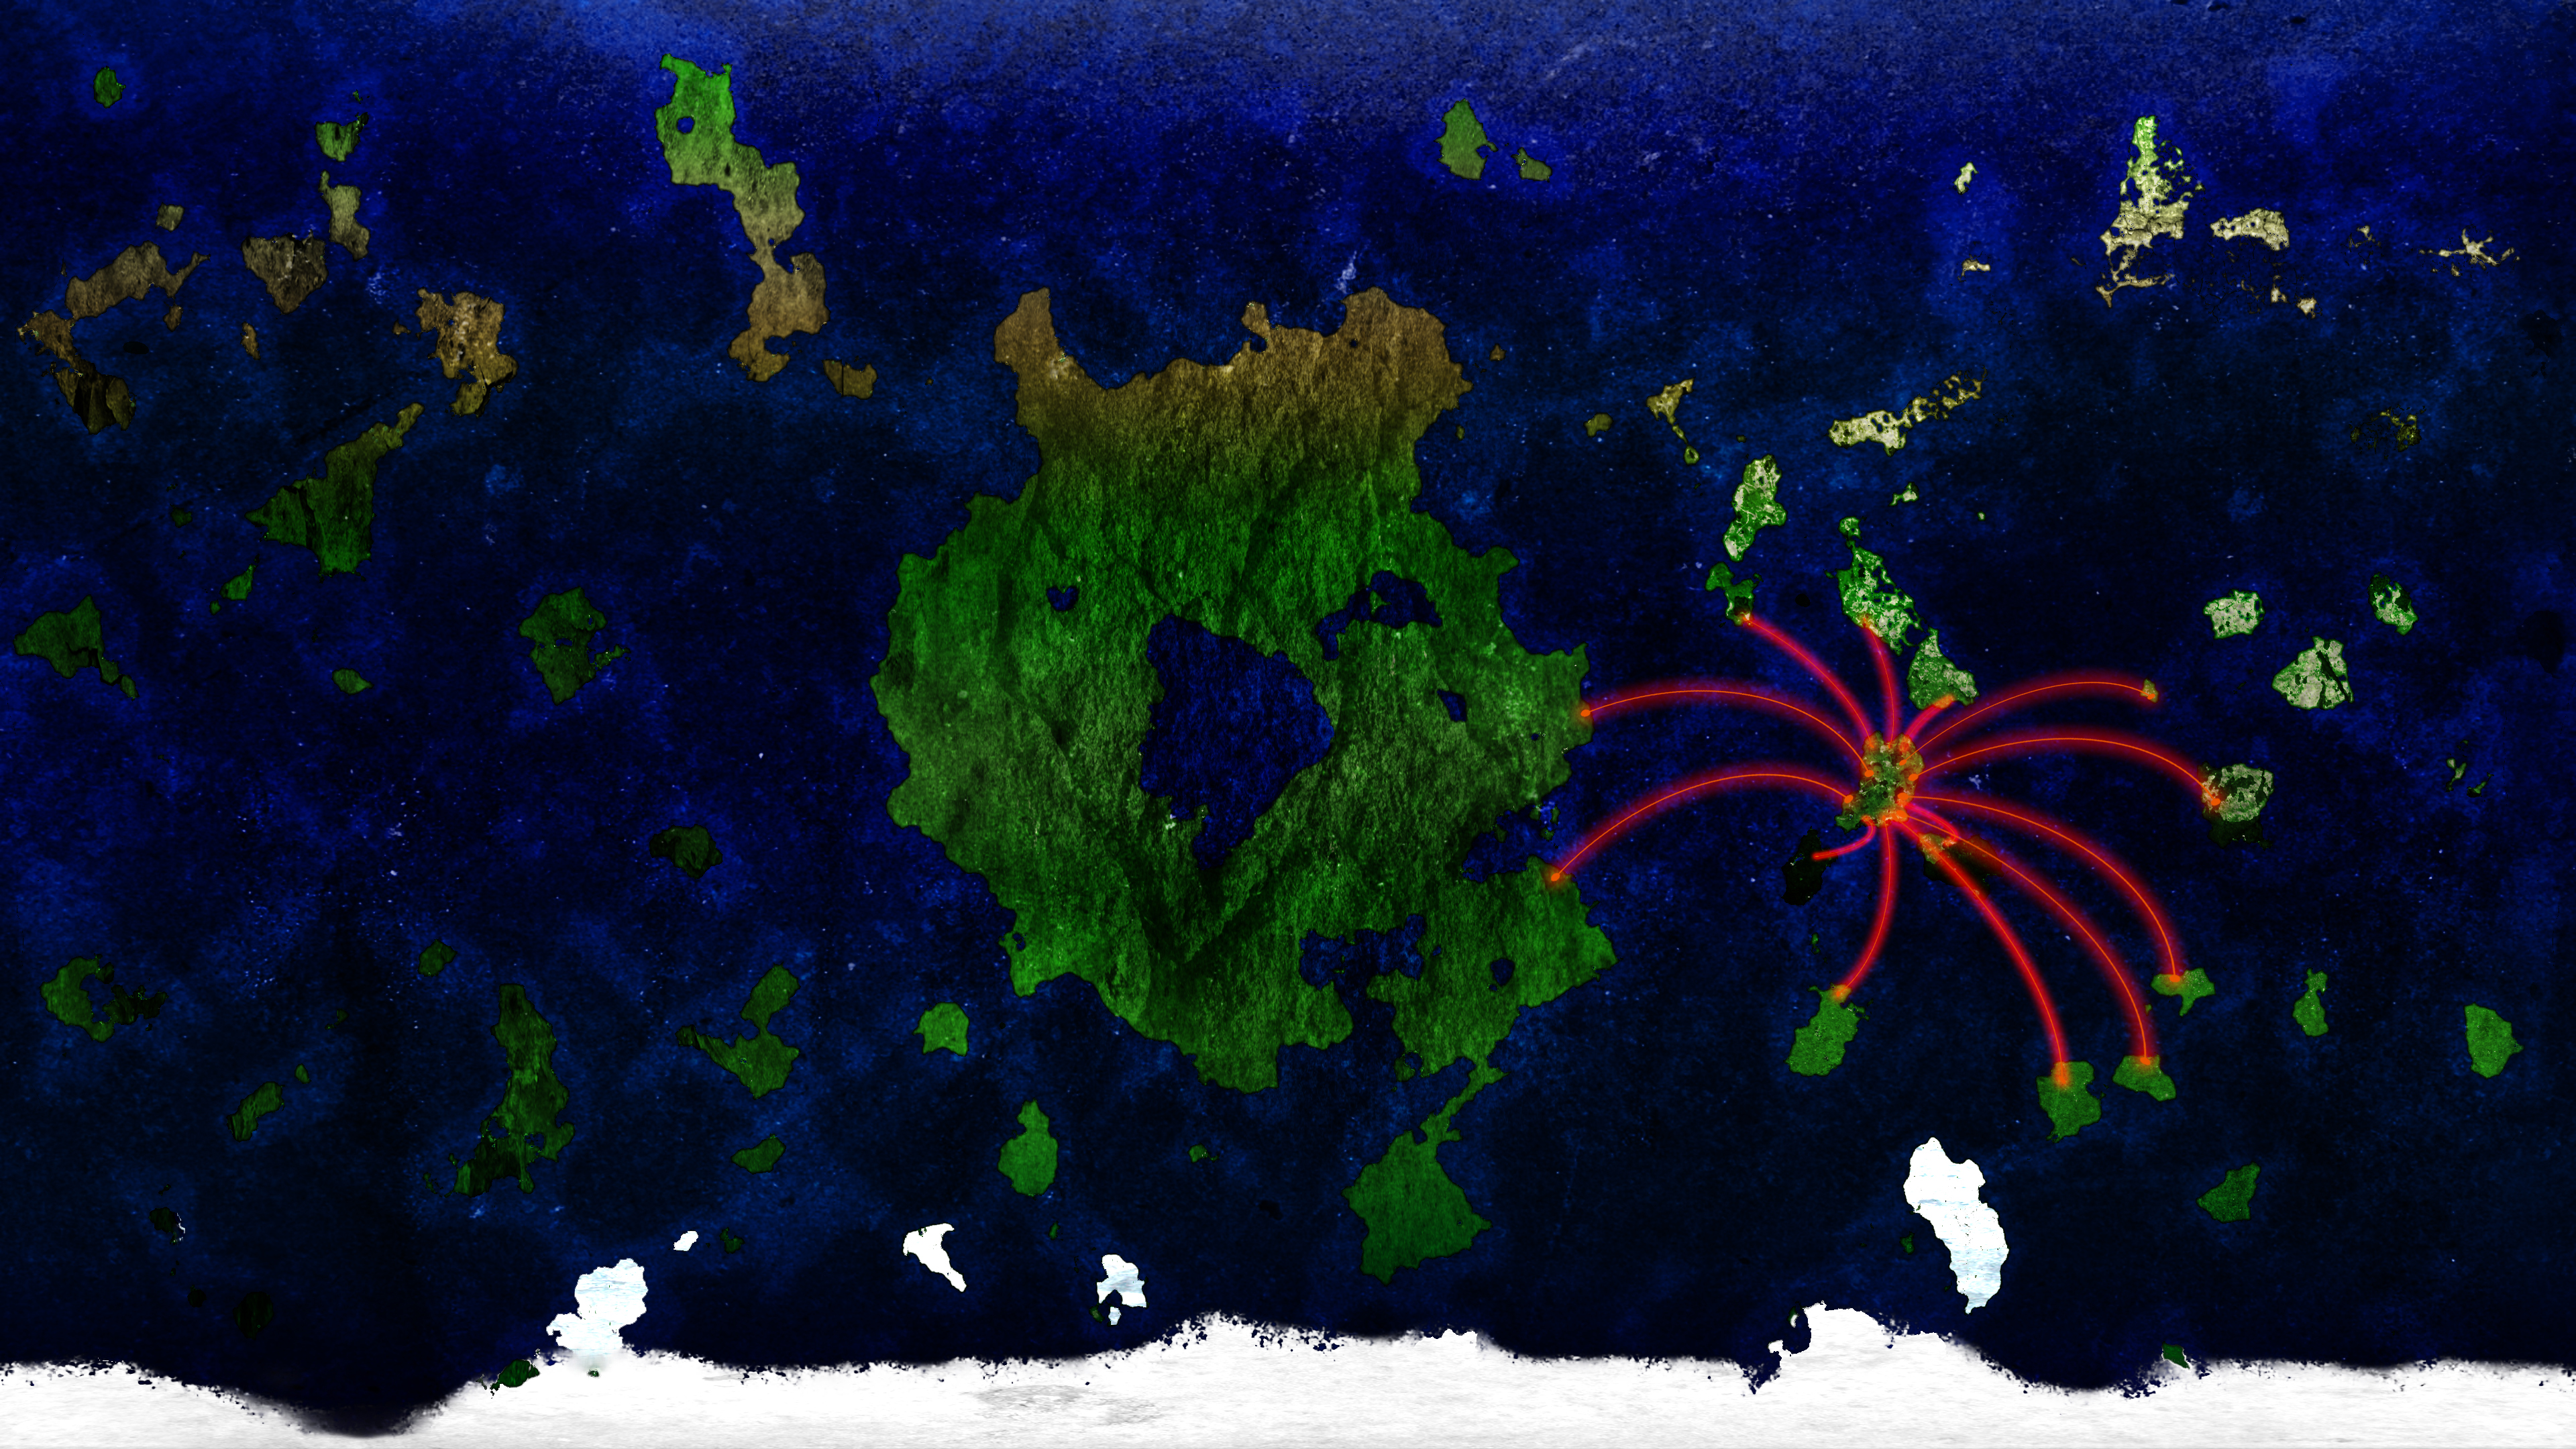
\includegraphics[width=0.48\textwidth]{img/CelestialConquest/OrillaCrusade.jpg} 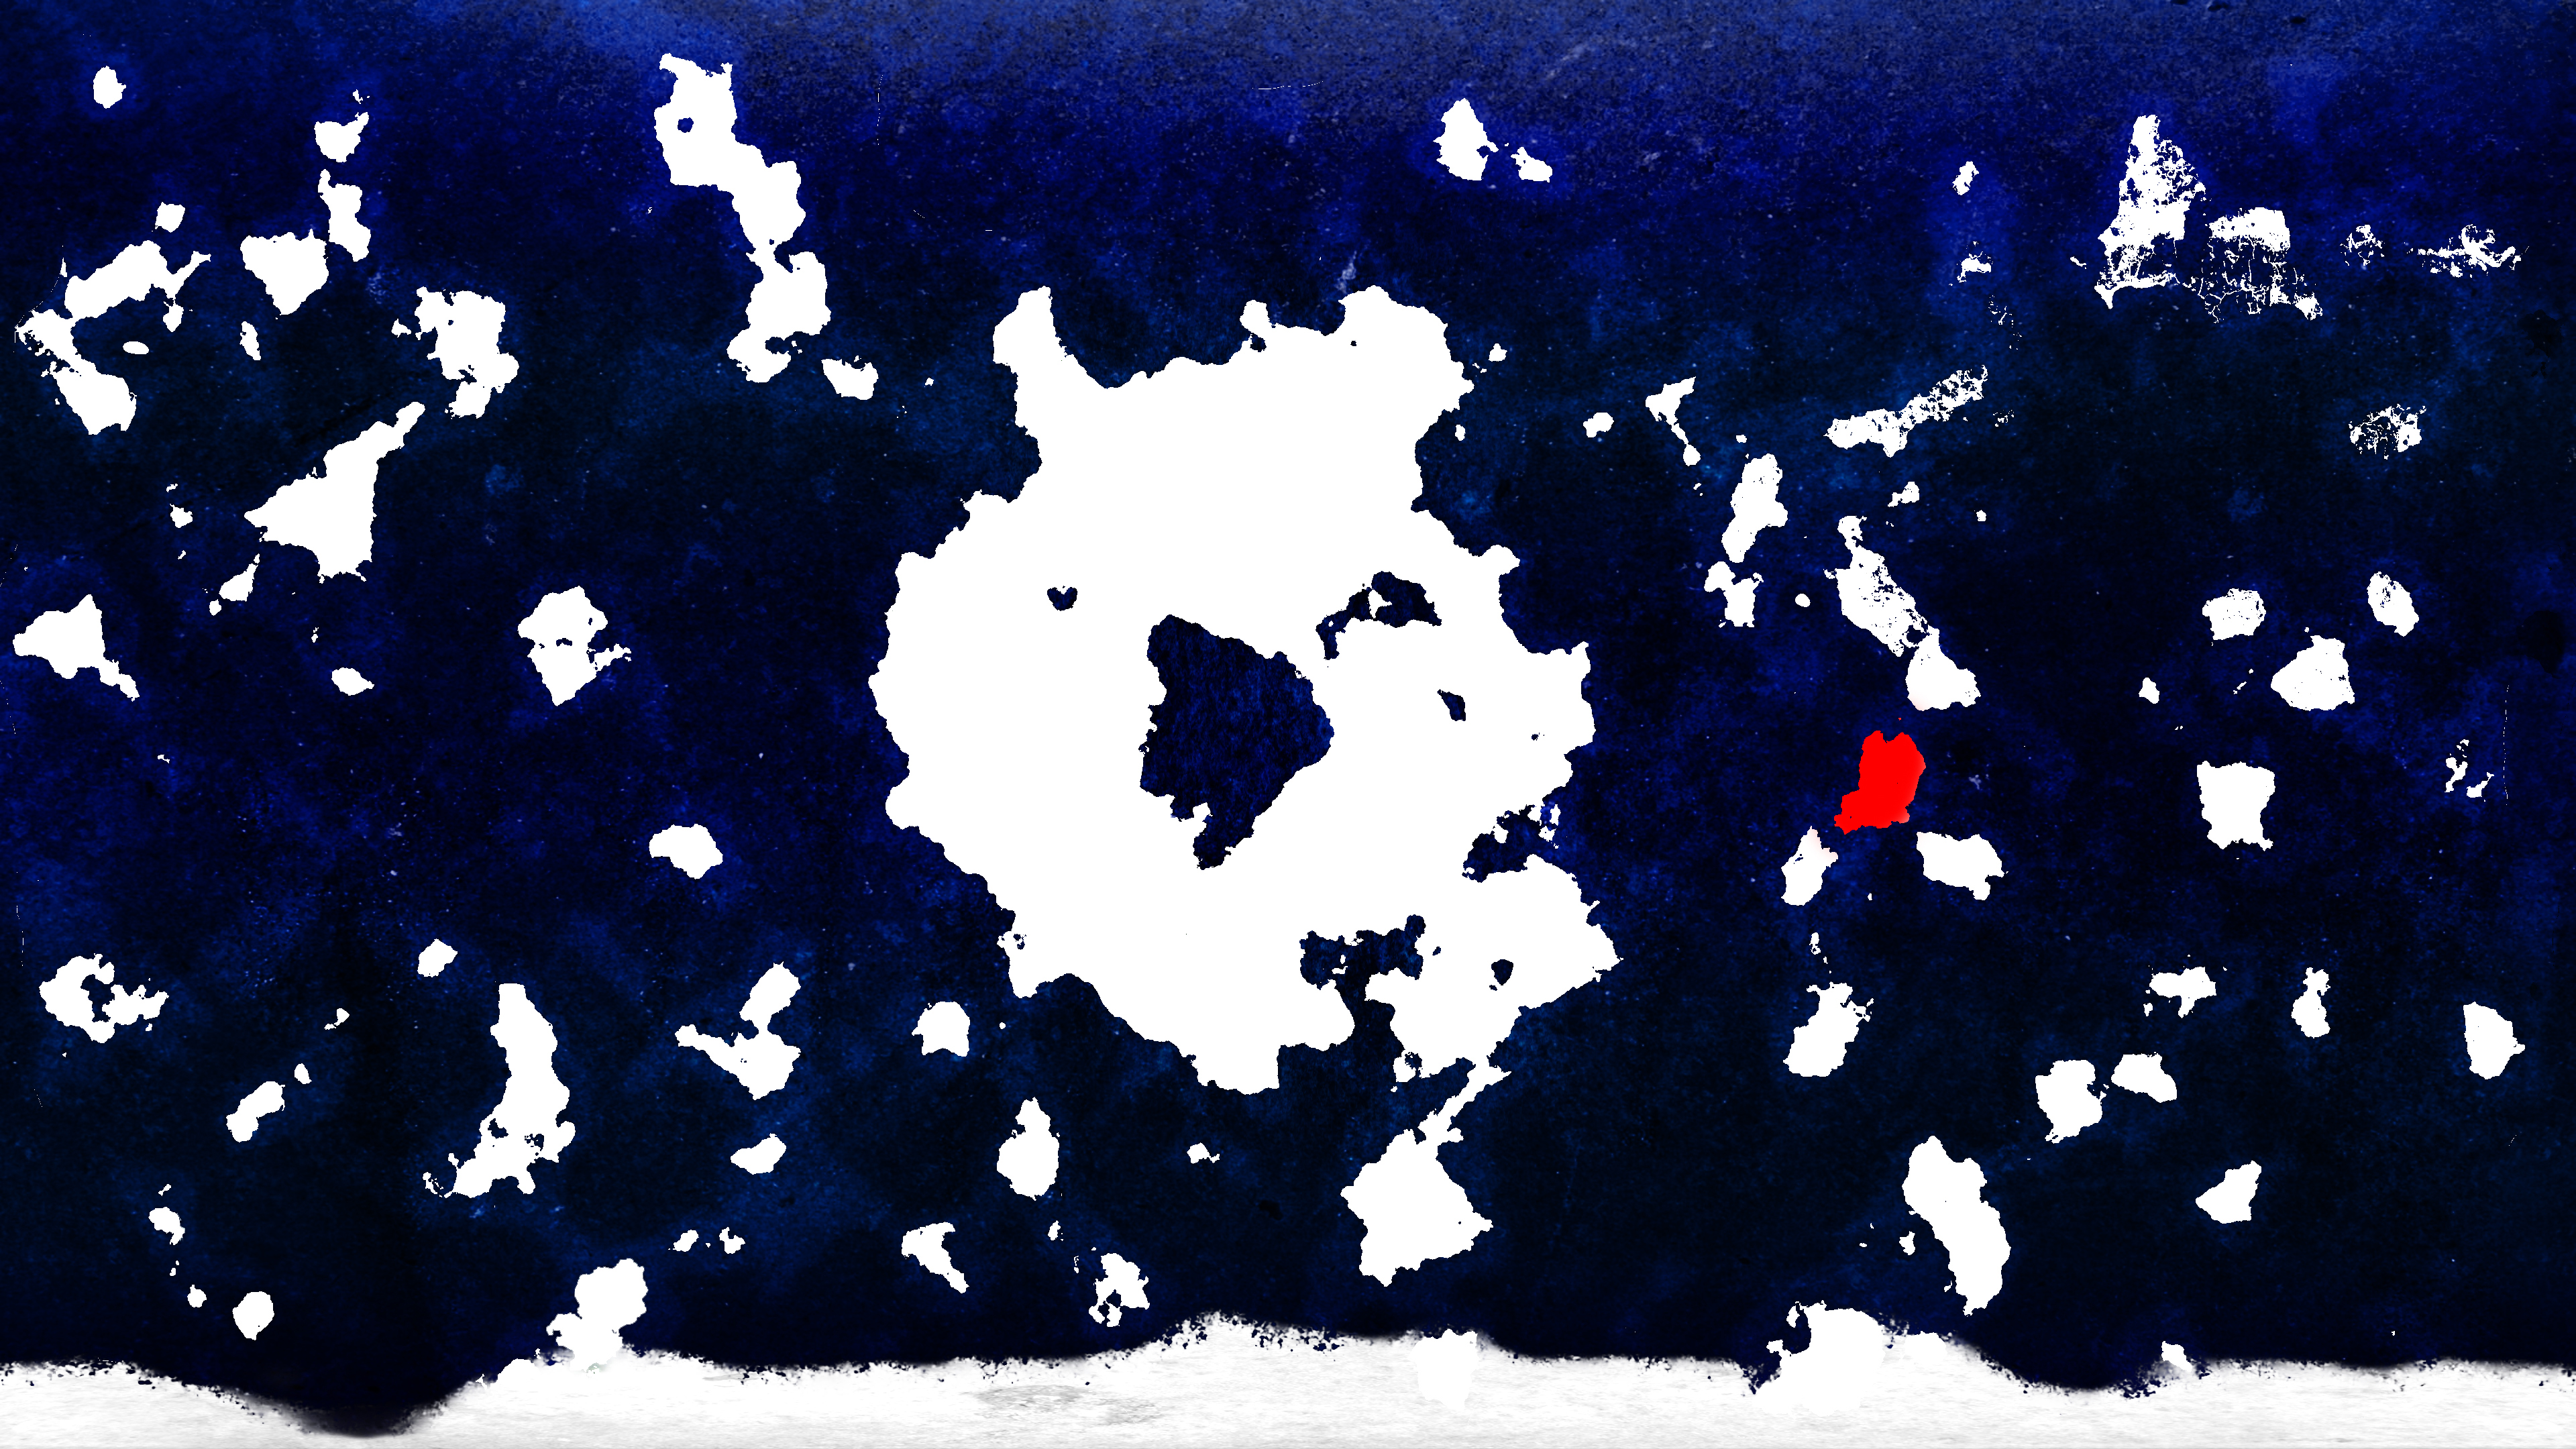
\includegraphics[width=0.48\textwidth]{img/CelestialConquest/CelestusConquest00.jpg}
		
	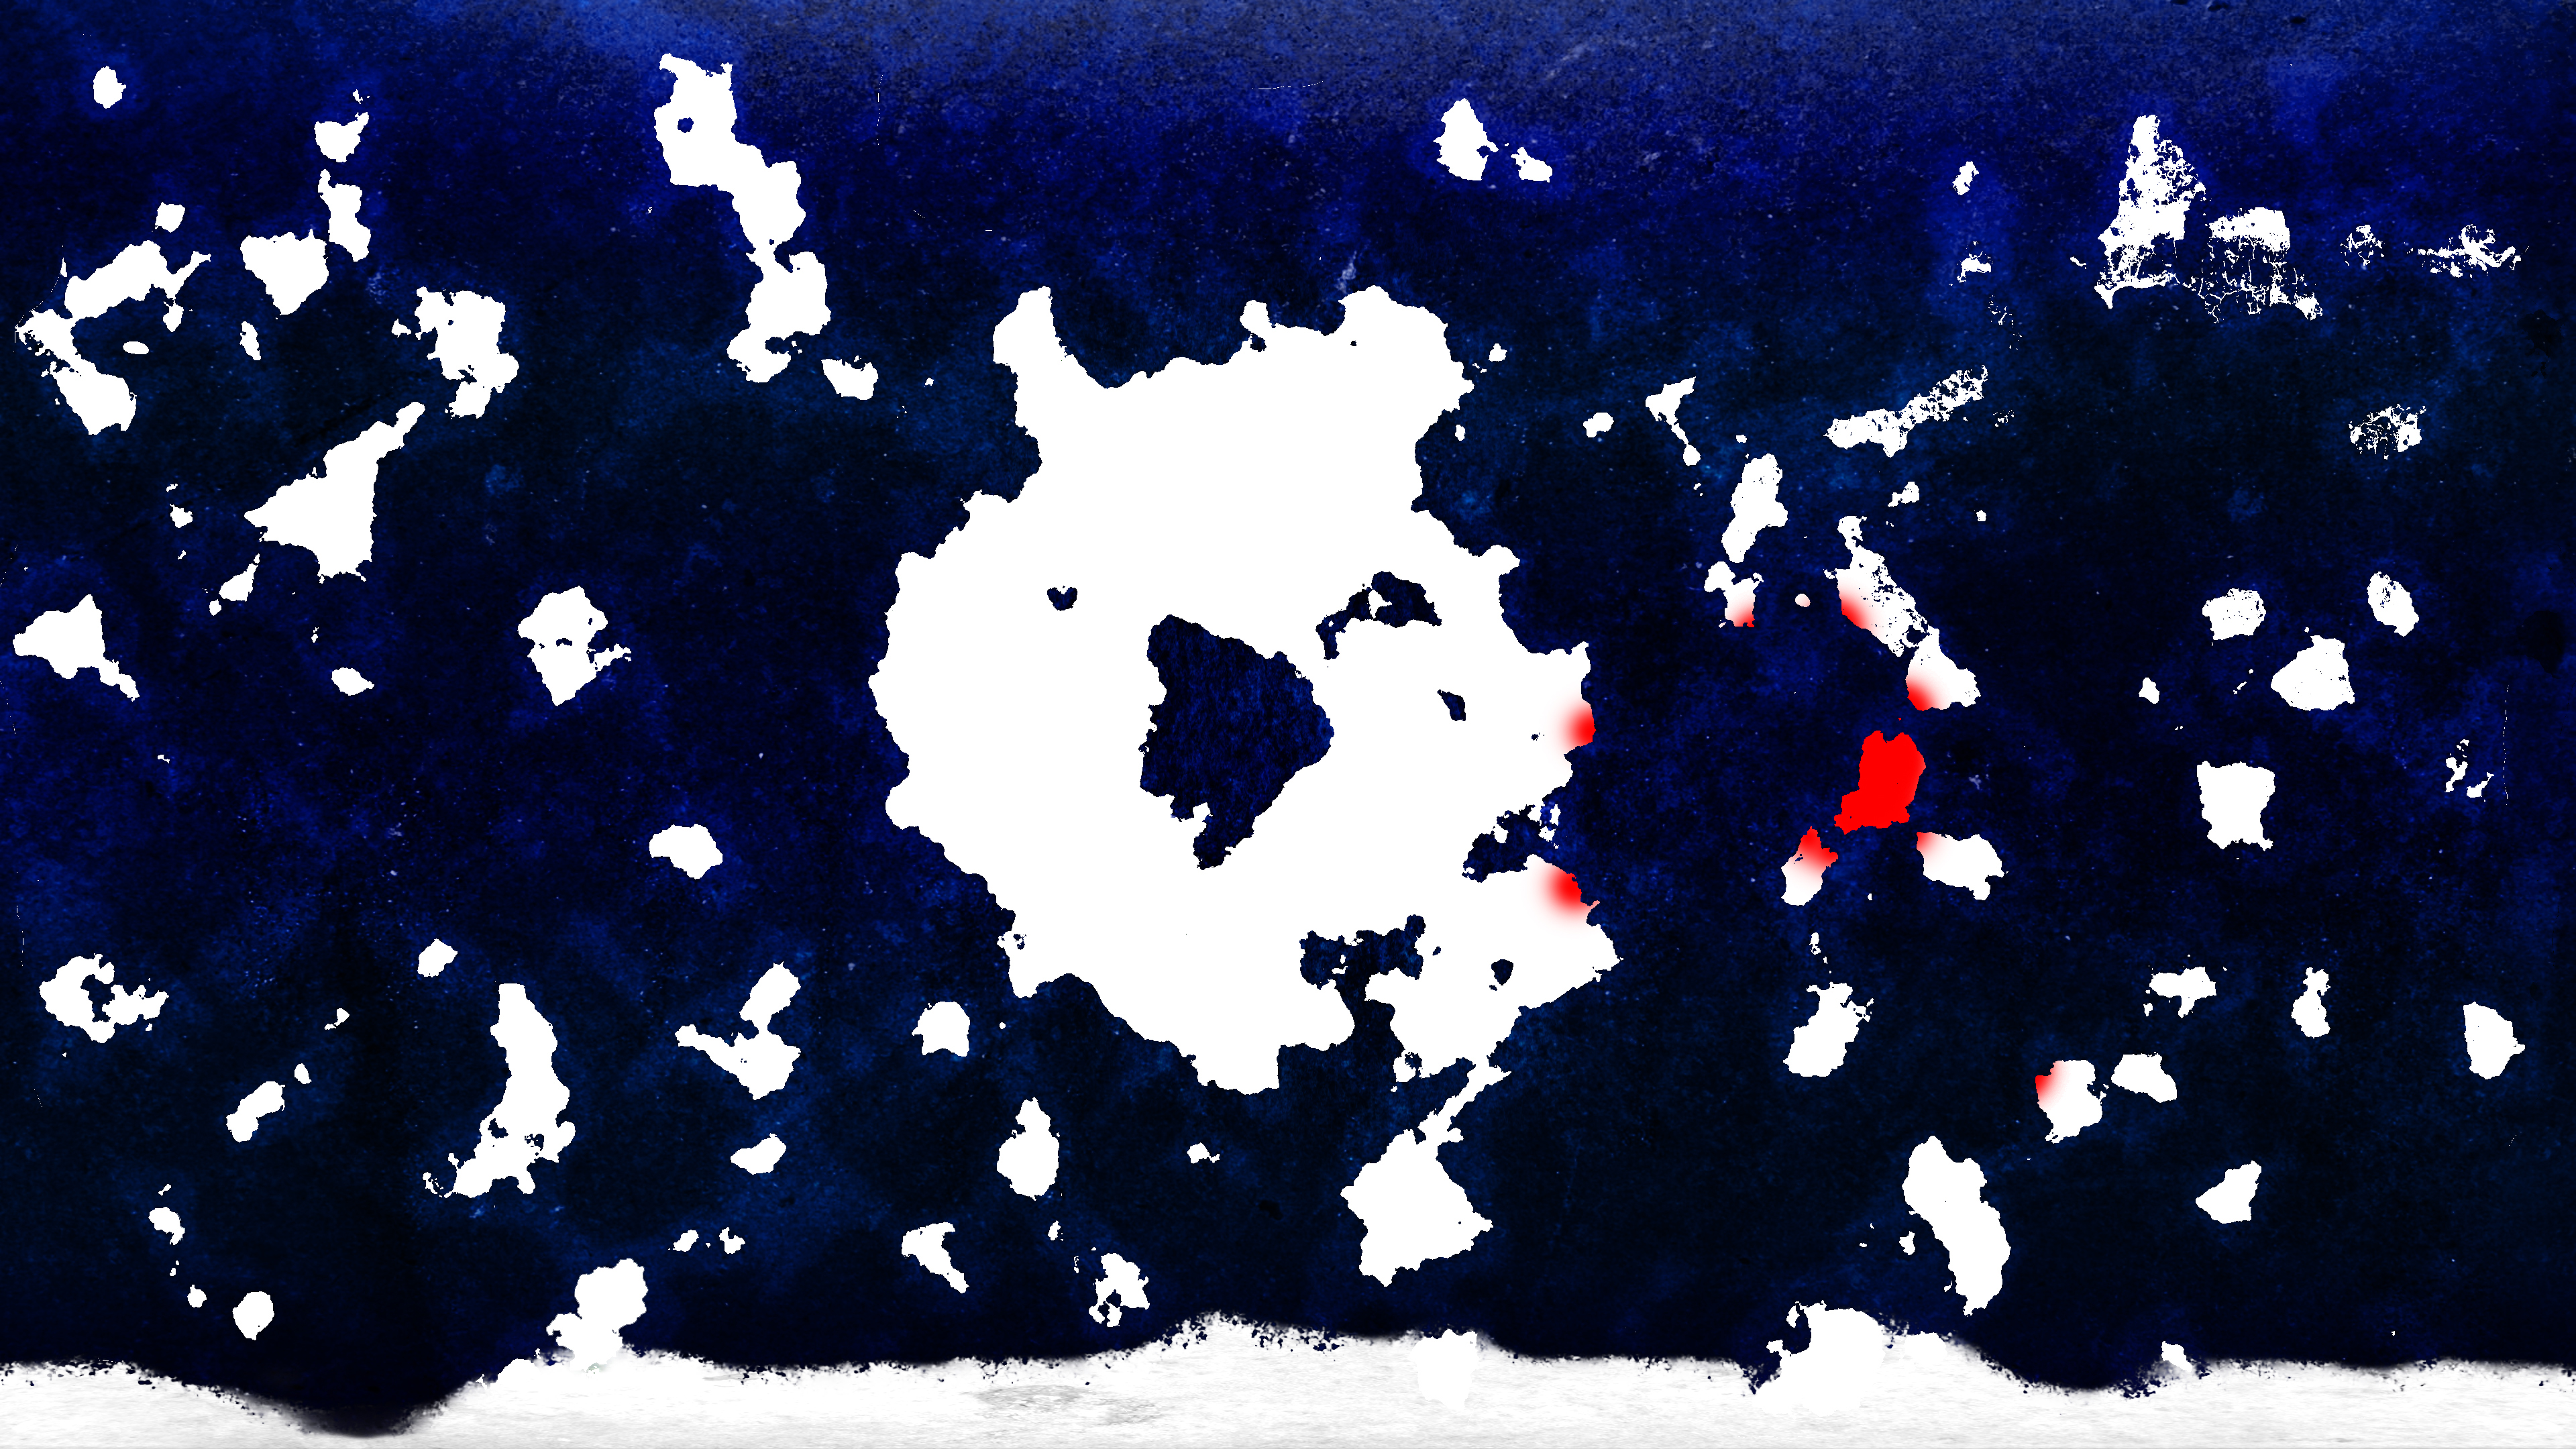
\includegraphics[width=0.48\textwidth]{img/CelestialConquest/CelestusConquest01.jpg} 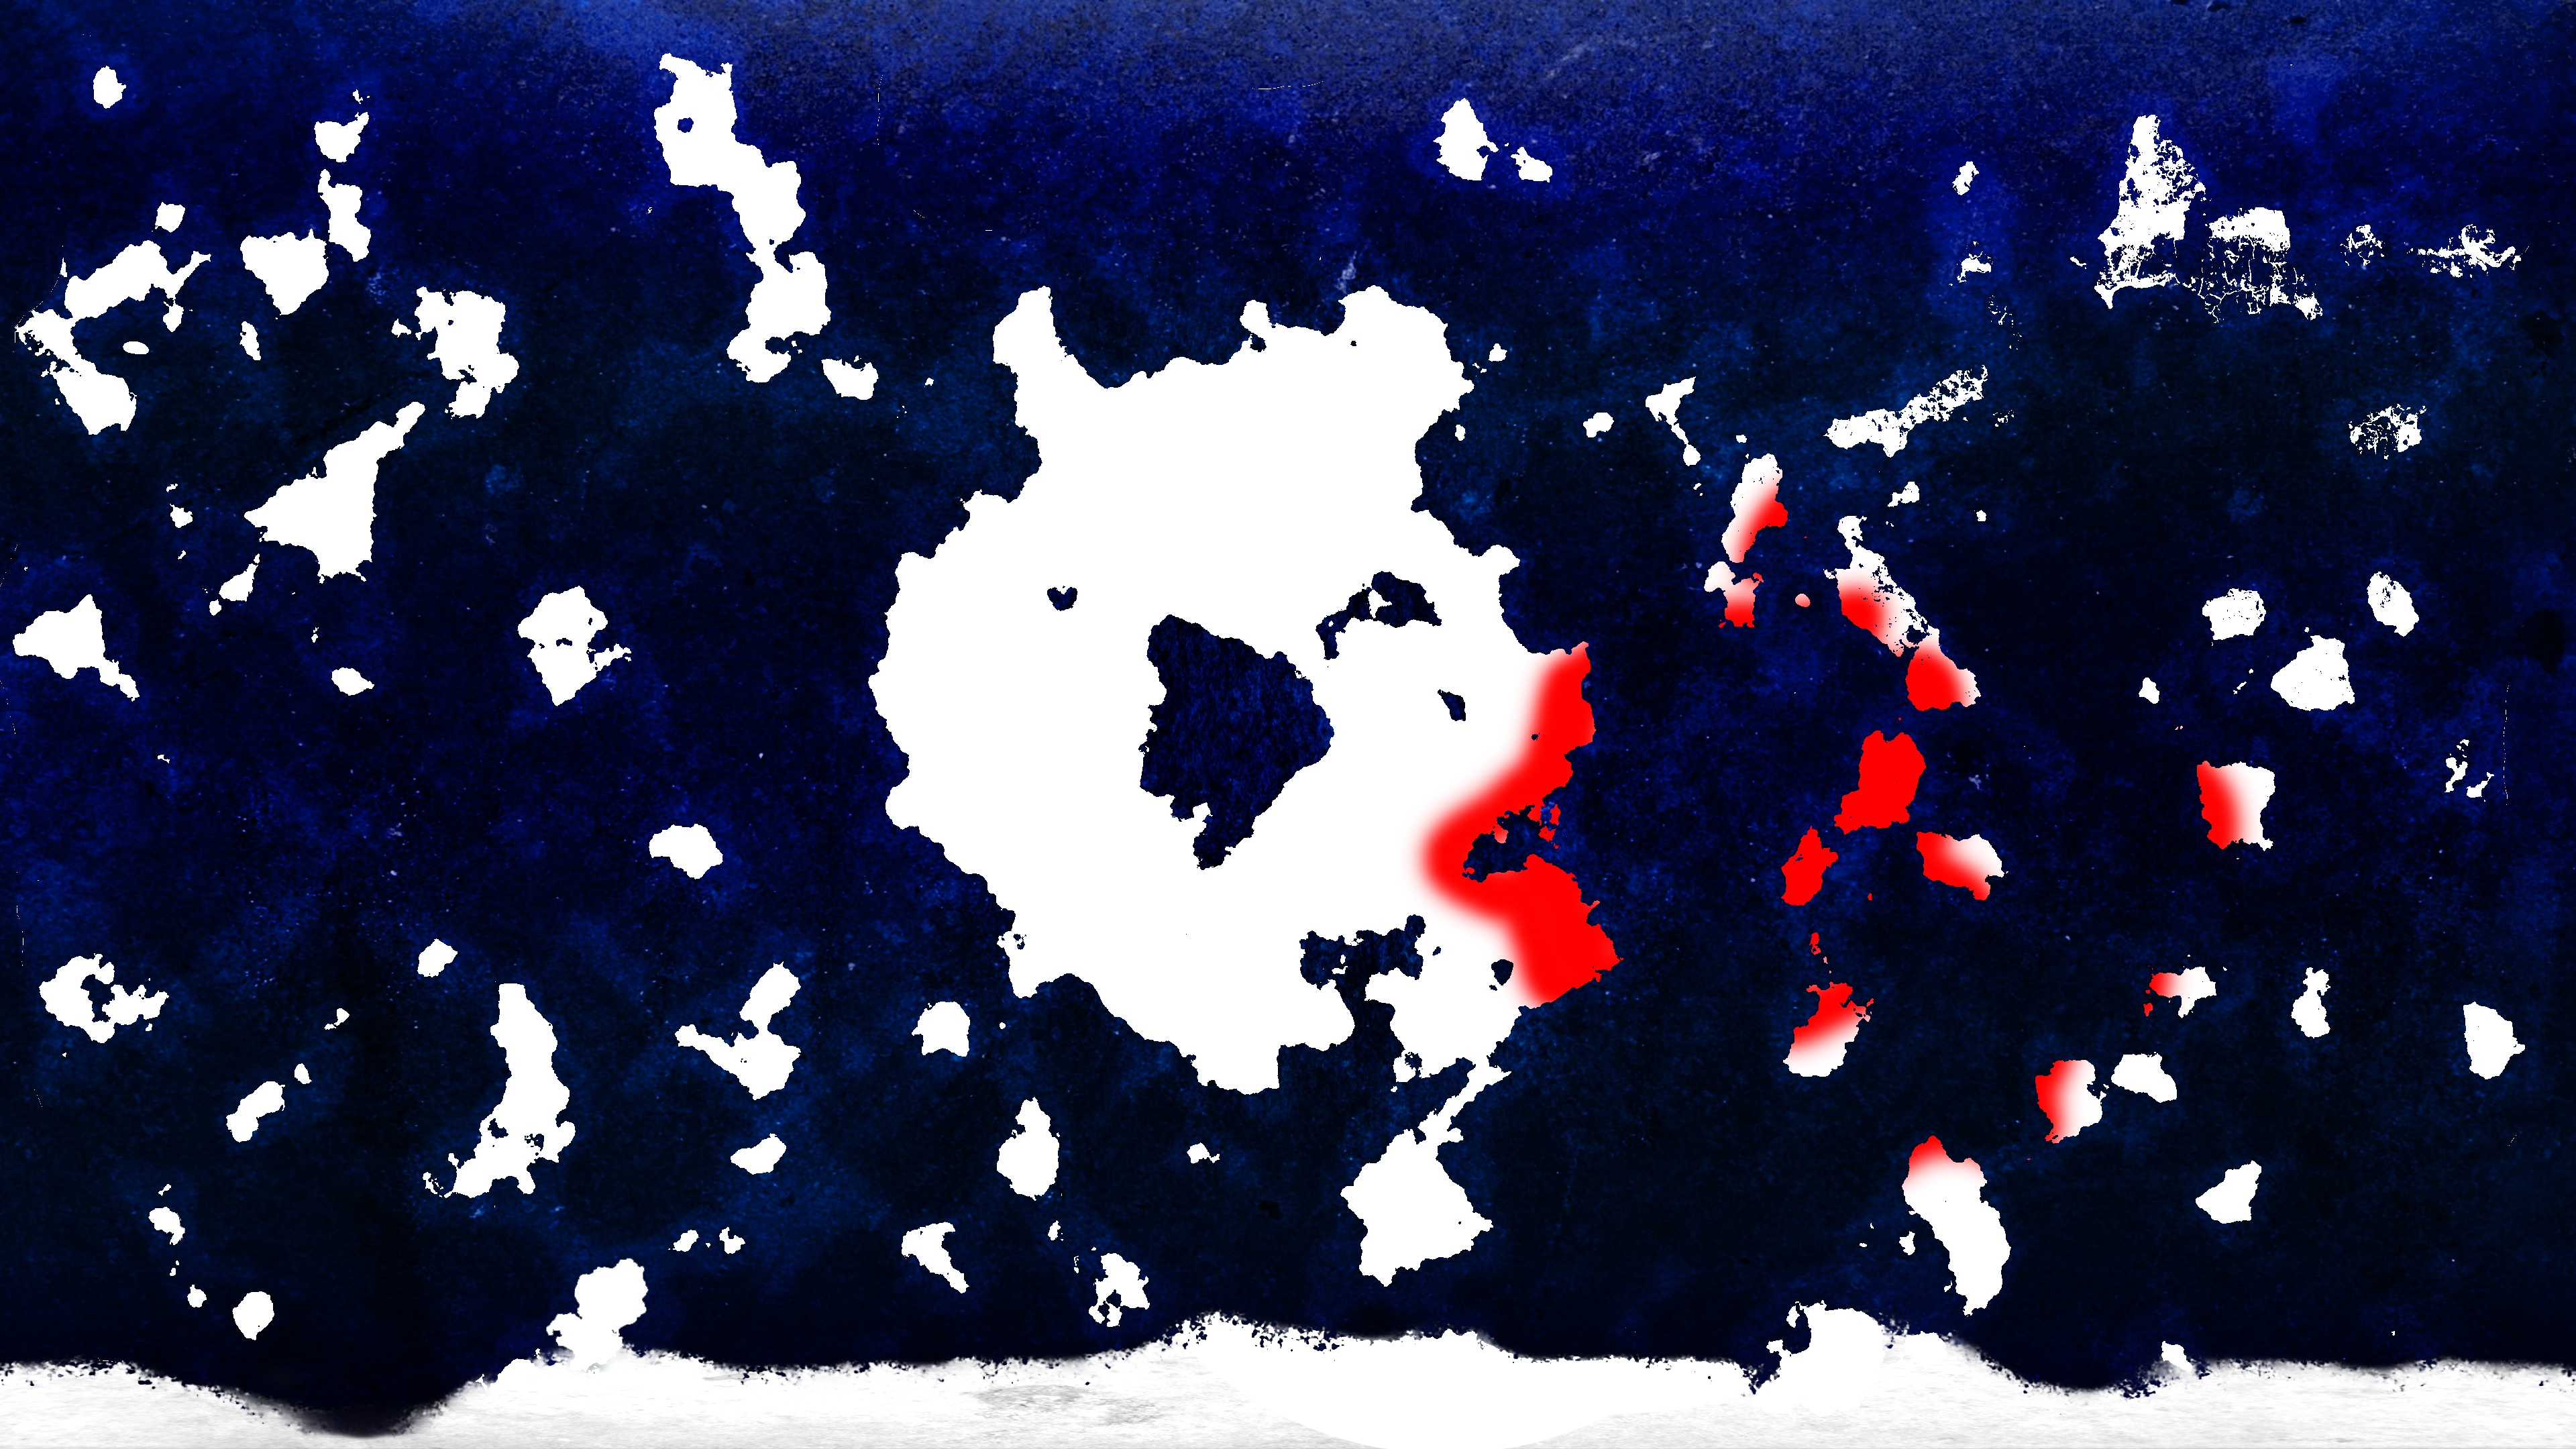
\includegraphics[width=0.48\textwidth]{img/CelestialConquest/CelestusConquest02.jpg}
	
	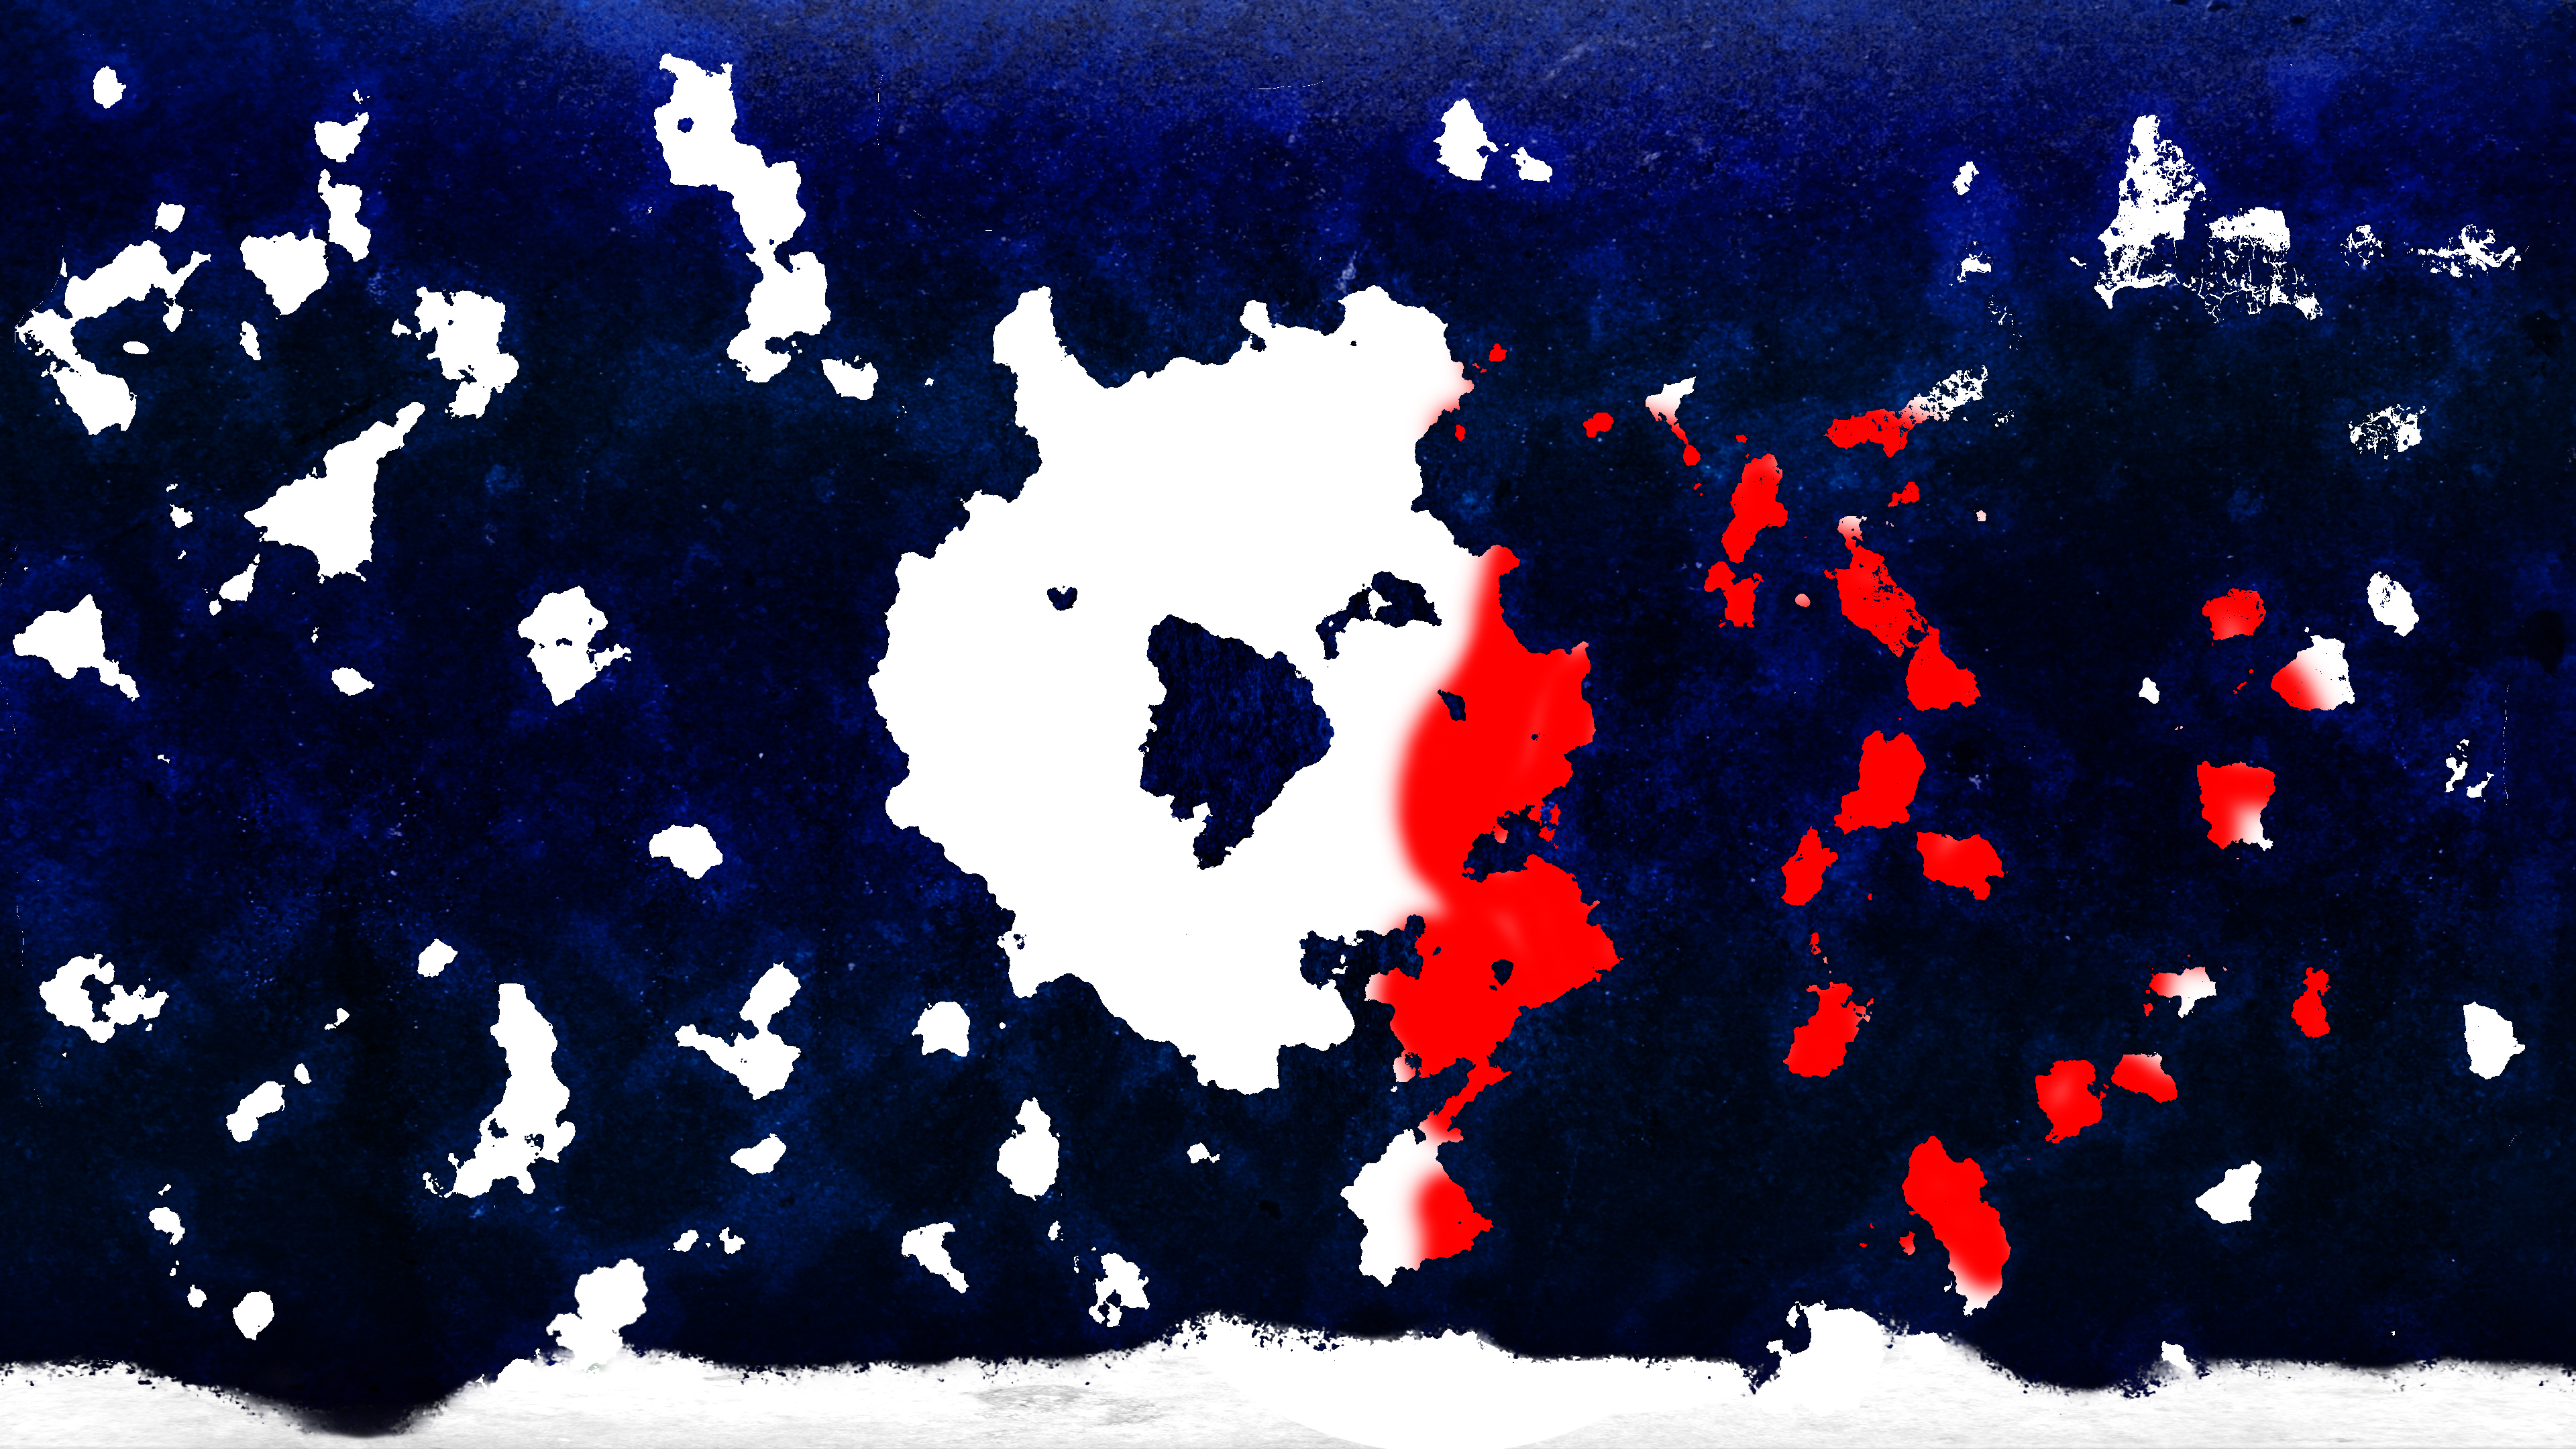
\includegraphics[width=0.48\textwidth]{img/CelestialConquest/CelestusConquest03.jpg} 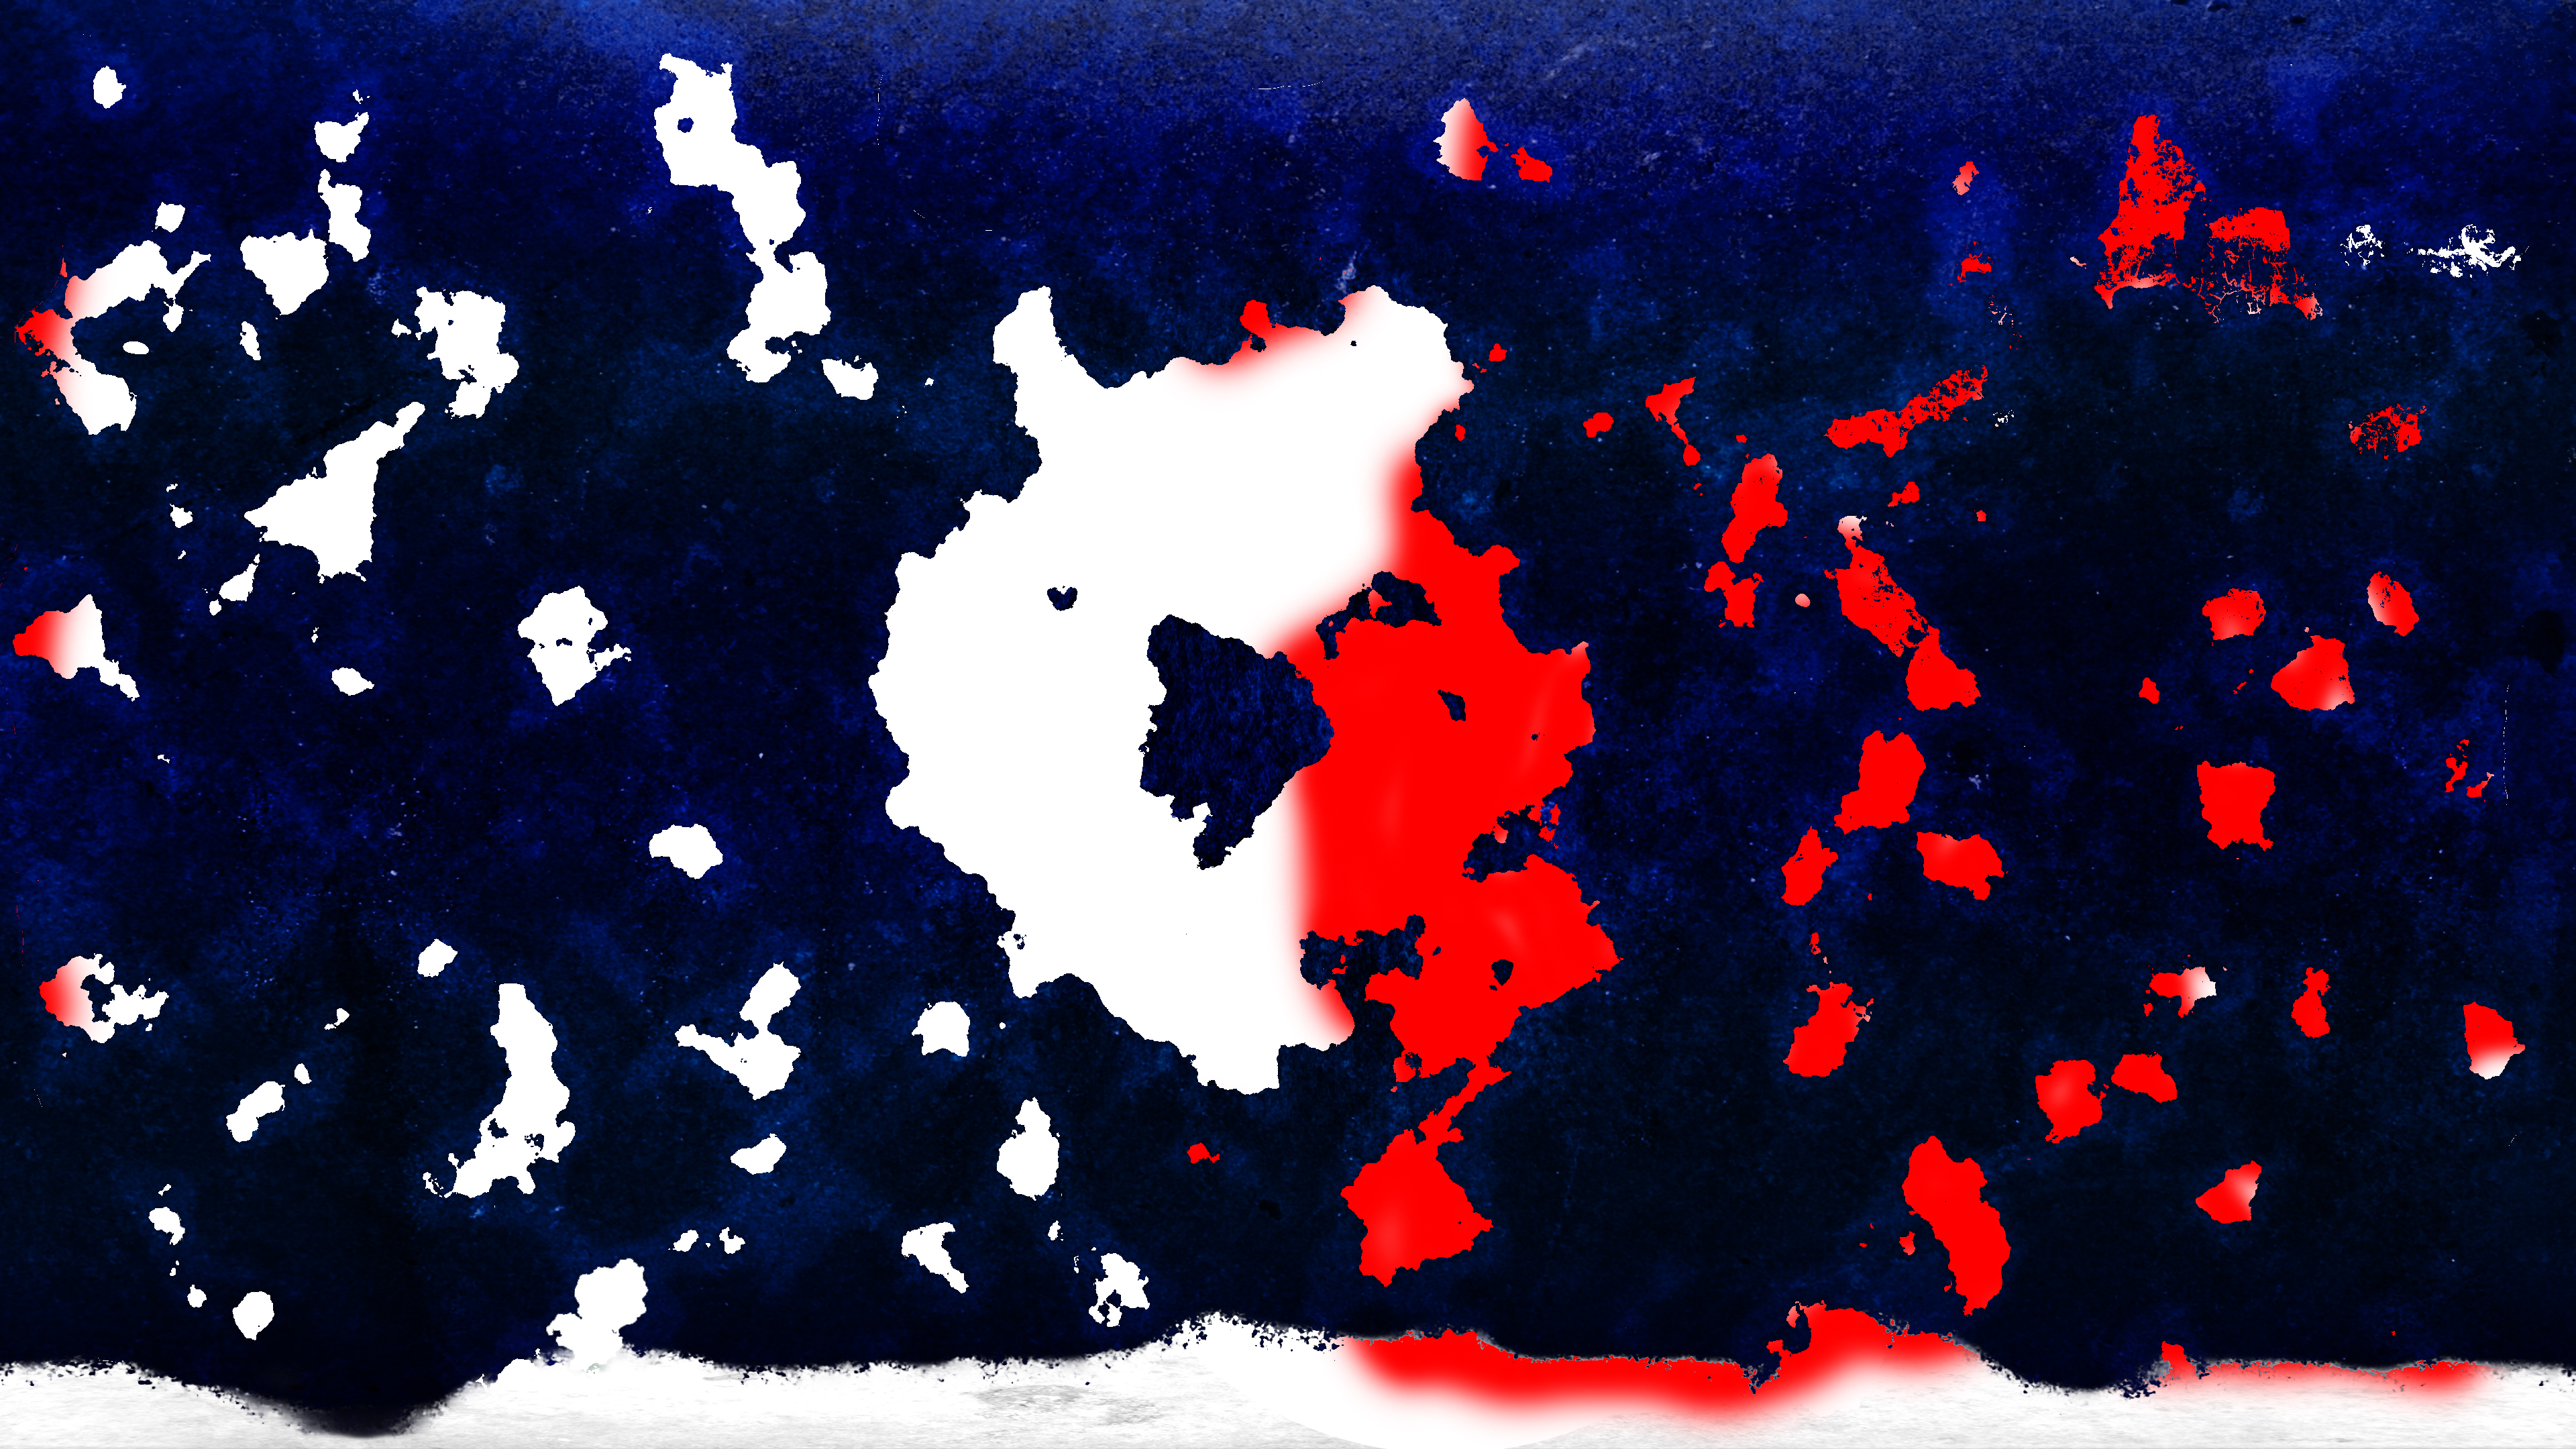
\includegraphics[width=0.48\textwidth]{img/CelestialConquest/CelestusConquest04.jpg}
	
	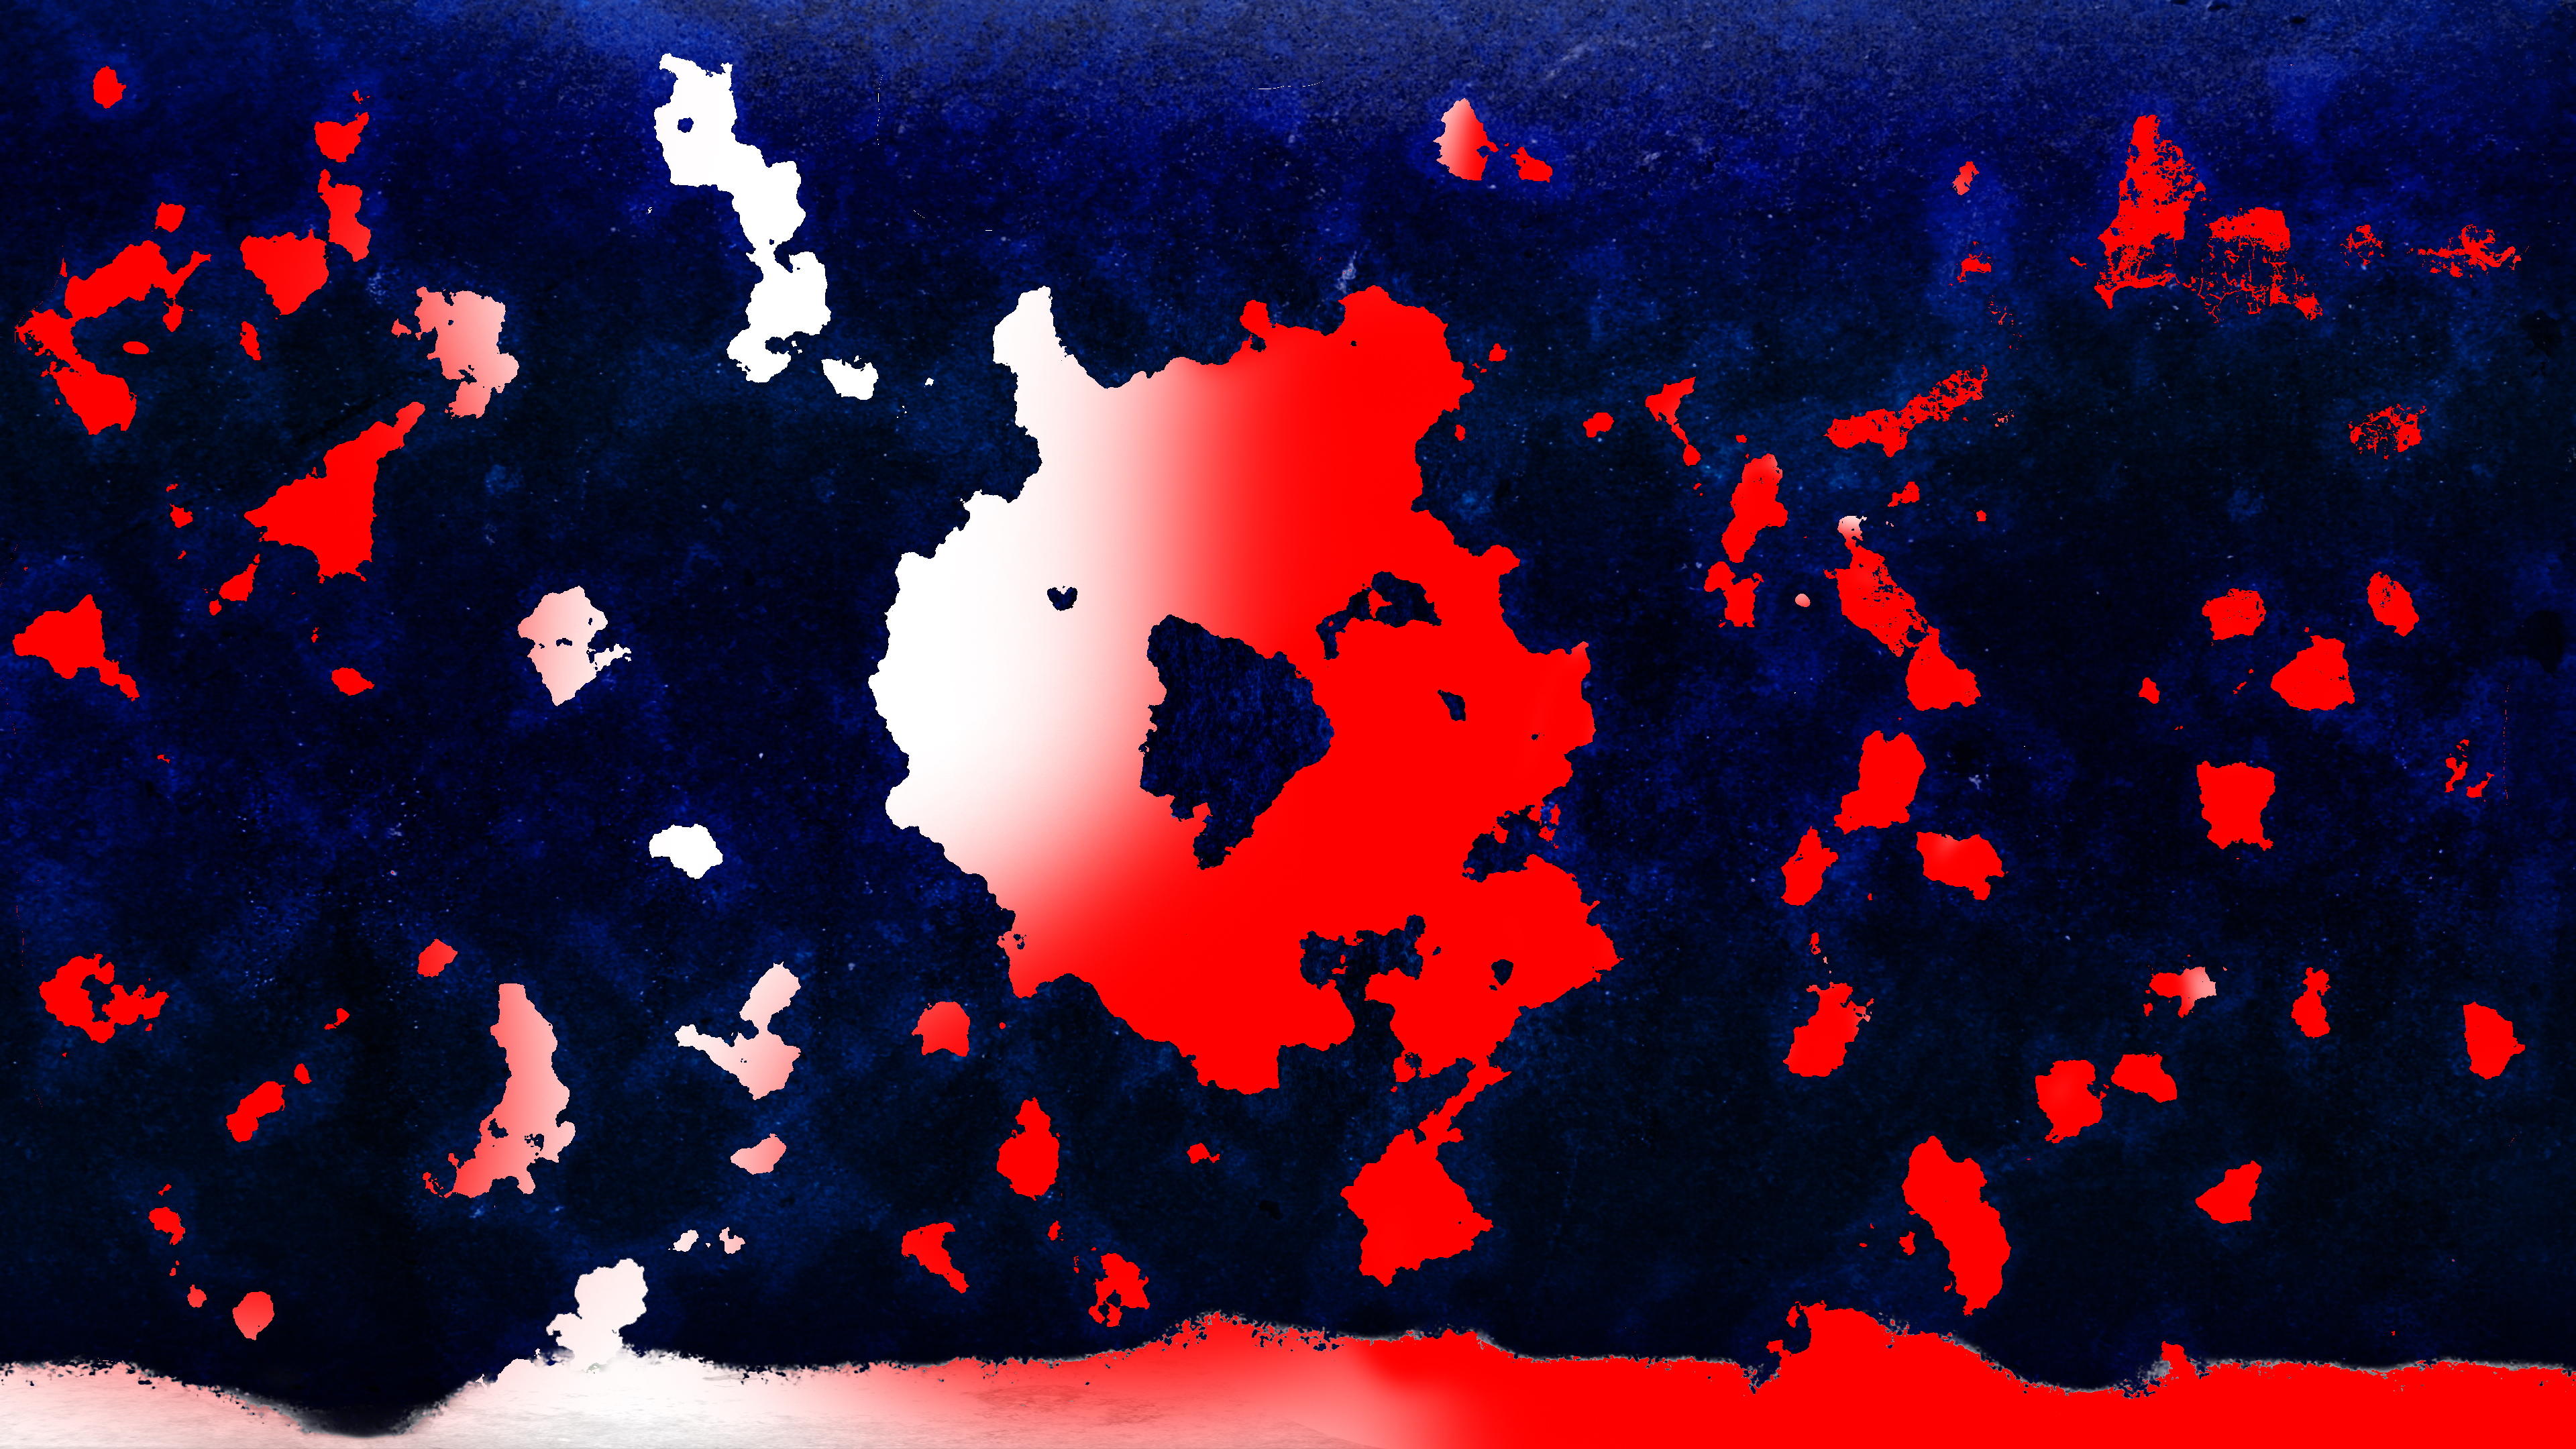
\includegraphics[width=0.48\textwidth]{img/CelestialConquest/CelestusConquest05.jpg} 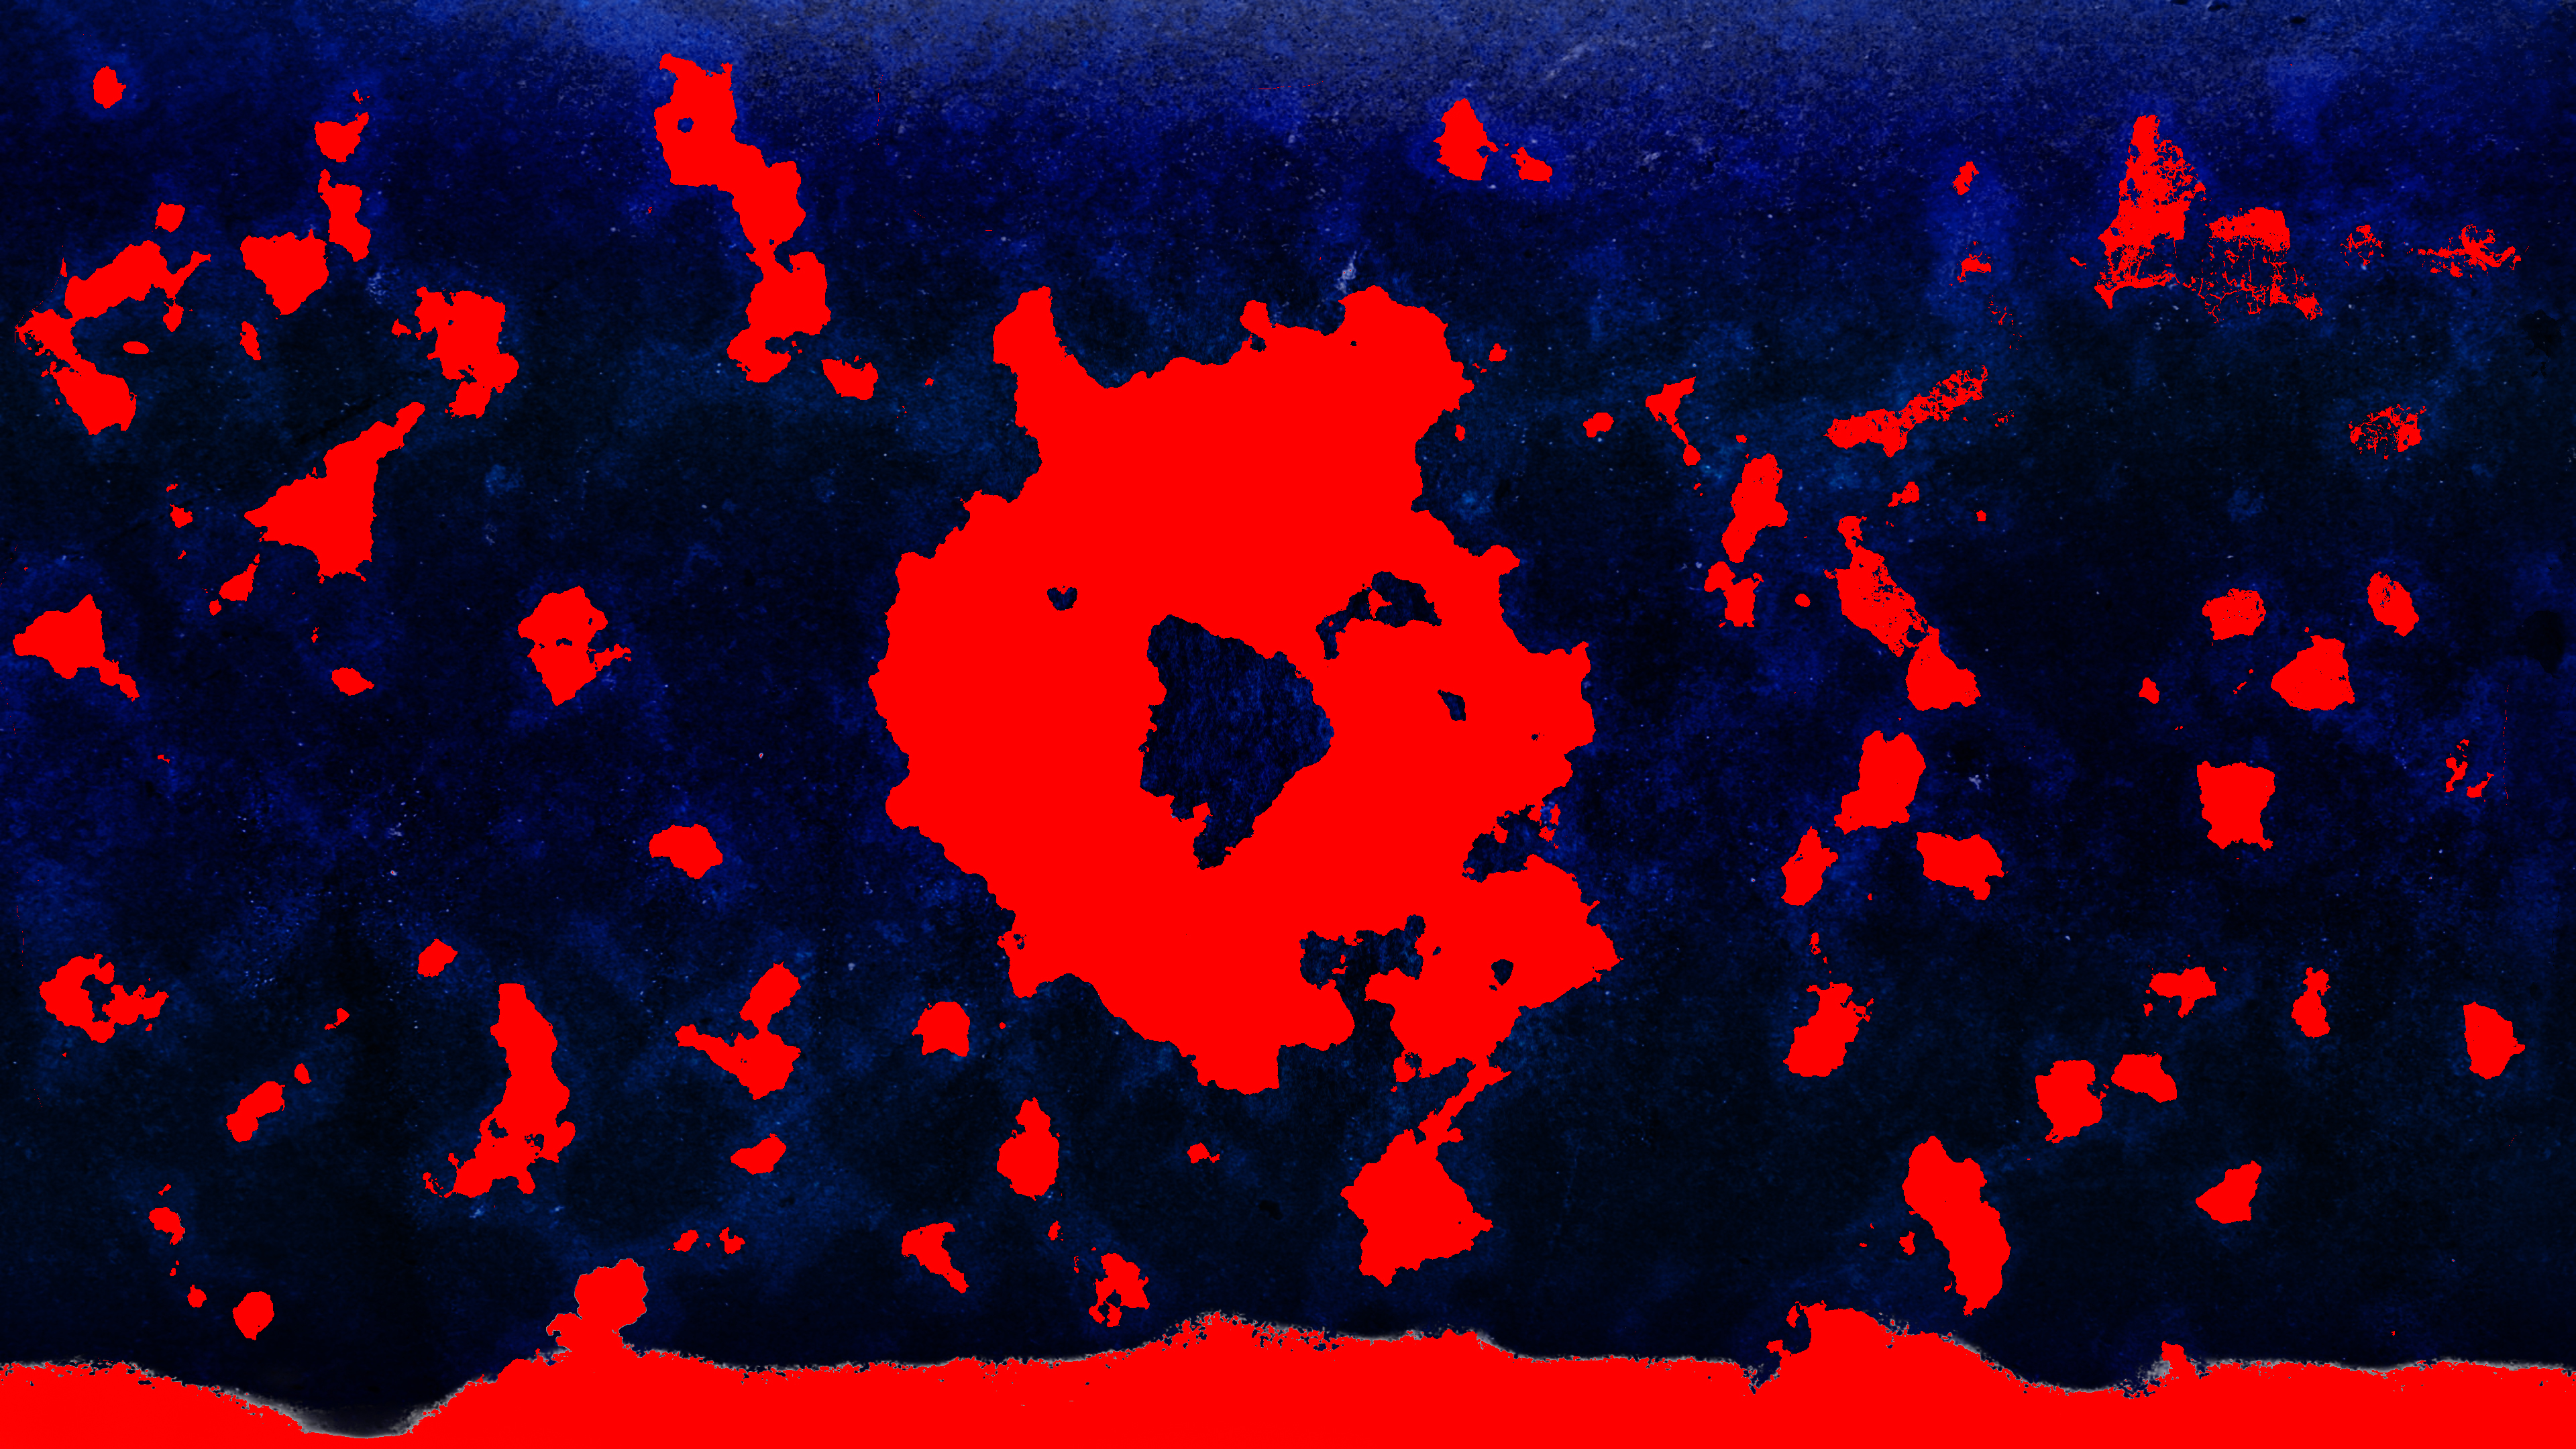
\includegraphics[width=0.48\textwidth]{img/CelestialConquest/CelestusConquest06.jpg}
\end{center}



\section{Myrddin}

Myrddin was an Alteran. His name, Myrddin can also be translated to Merlin, regarding Merlin and the knights of the round table. Merlin was a member of the Celestial guard whom figured out the secrets to ascension but saw the negative consequences it could have on the planet and universe. He decided to not ascend himself and instead rebelled against the Celestials. In doing so, none of the other Alterans (the ones who could ascend) stayed with Merlin and he was left alone with his beliefs. Myrddin was one of the first to determine the secrets behind ascension and was one of the most knowledgeable of people at that time. Some of the other Alterans ascended and took off deep into the universe while others became their own `gods' throughout Orilla.

Myrddin put it upon himself to create a technology allowing him to destroy ascended beings, which was not thought possible. However, he could not do such a thing outright because the Alterans and Celestials would have interfered and destroyed him, but instead he had to find a way to mask his work by shifting himself between dimensions continually. Do do so, Myrddin had to uncover the secrets of the legendary Trinity Stones, which he was able to do. He found all three by solving the riddles left to conceal them and used them to guide his own understandings of reality.

He was able to create a device known as the San'graal (The Holy Grail) which had the capabilities of destroying the Celestials but was unable to activate it due to him closely being watched by the Celestials. Myrddin instead left his work hidden behind secrets, like the Trinity Stones and kept his secrets safe guarded by the knights of the round table throughout the generations.

Myrddin's end research was left in a secret lab which can only be accessed via the Trinity Stones. Myrddin froze himself in stasis within his lab and he contains the knowledge of how to create the San'graal by it's base particles. If the Trinity Stones are pushed together (after being found of course), the users will be transported to Myrddin's Laboratory on one of the moons of Orilla. Myrddin and his various other labs were all located on this moon and in the Pluvian Forest. One of such places is referred to as Avalon which is a place where him and his knights kept all of the treasures from that age.

\section{Xur'la}

Xur'la is a physical god created by Myrddin\footnote{Physically modeled after the Naaru from World of Warcraft}. Xur'la was created by Myrddin to be a half-ascended and half-physical being. He created Xur'la to mask the Pluvian realm from the Celestials and other gods. Xur'la is a being that exists hidden within the Pluvian realm and continually modifies the spiritual properties around the Pluvian realm to mask the region from outside ascended beings. One of Samilah's (who is the daughter of the Celestials) goals is to find Xur'la and corrupt the physical side of it to diminish its power and allow the Celestials to penetrate the barrier that is the Pluvian forest. If Samilah manages to find Xur'la, she can corrupt it which will changes it's appearance to be that of a dark being.

\begin{center}
	\includegraphics[width=0.49\linewidth]{img/WoW/LightMother-5.png} 	\includegraphics[width=0.49\linewidth]{img/WoW/LightMother-4.png}
\end{center}

\section{Morgana}

Morgana (also known as Morgen La Fey where La Fey means the fairy) was an Alteran from Myrddin's time. She was greatly opposed to Myrddin advancing his capabilities to combat ascended beings due to her plans to ascend herself. Unfortunately, due to herself convincing that Myrddin succeeded in creating the San'graal, she never ascended herself. She dedicated her life to studying the Trinity Stones and to determine Myrddin's secrets to destroy the San'graal before ascending. However, during her lifetimes, she was able to understand the true threat that the Celestials posed and changed her mind to side with Myrddin. Myrddin was significantly more clever than Morgana and Morgana determined that there were safeguards around the San'graal preventing her or ascended beings from finding it. Due to this, she planned to lie in wait to assist those who can actually find it. 

\subsection{Morgana Lore in the Campaign}

Morgana, also known as Morgan the fairy was a powerful enchantress in the Arthurian legend. She was a goddess, a sorcerer, benevolent and related to King Arthur, as his magical savior and protector. In many of her iterations, she has potential for both good and evil. Her prominence increased over time and some sources portray her in a cyclical prose such as the Vulgate cycle. The Vulgate cycle ands dimension to the King Arthur tradition, and the birth of Merlin as the son of a devil who gained the ability to see future events after transforming into a prophet. The earliest account of her equates her with the isle of apples (Avalon). which is where Arthur was taken after being fatally wounded. These claim she was removed from goddess status and became a mortal but retained all her powers.

 



\chapter{The Campaign}

\subsection{Tempestas}

At the start of the campaign, the DM needs to decide on a reason for the characters to be coming into Tempestas. This can be any good reason that fits with the player backstories or one from the following list. Tempestas is a large city with many things to do. The city will start closed off due to the impending threat of the Celestials attacking nearby cities. From Tempestas, the players can be lead to Aurushire. Different reasons can lead them to Aurushire such as the sport of the jungles or the search for the Trinity stones. Little do they know that the Trinity stones are the key to obtaining the San'graal to defeat the Celestials.

The players can start out in Tempestas either by living there, being in the prison there, or arriving there by spice trade (depending on the character backgrounds). While in Tempestas, they can encounter a few important characters such as Dastan and the fortuneteller. While in Tempestas, a Prior of the Celestas will also arrive and start his preaching. 

\subsection{Journey to Aurushire}

\begin{commentbox}{Journey to Aurushire}
	\begin{description}
		\item[For the Stones] Legend has it that there are rare and priceless artifacts hidden on Statu. It is possible that the player could be hunting the legends which have lead them to Aurushire.
		\item[The Rare Sport of Rem Silva] It is possible that the rare game in Rem Silva was spoken of and the players could be after the rare sport that resides in this area.
	\end{description}
\end{commentbox}

After leaving Tempestas by boat (If the party gets to this), they will have some rest time on the ship they are on. The tripe is generally only about a day or two away from Statu, however the party will encounter rough weather. The rough weather will turn into a massive storm in which the ship will be knocked around, back and forth. The party will be knocked unconscious and awake on the coast due east on Aurushire (without knowing of course) with only the players that are in their party and none of the NPCs from the ship. The cost will have rock and cliff faces to their east, and rough forest and mountains (appears unclimbable) to the North. Their only option is the the west. The west will lead into the Convallis swamp and marsh area's which is directly east of the Naga encampments. A thick fog will appear as they are traveling and they will need to navigate through rough swampy regions where they will encounter serpent Naga forces and some magical beasts like a witch hunter. After navigating through this region, the party will arrive and Aurushire, battered and beaten.

After arriving at Aurushire, there are many options for the players. There is an Inn (Prancing Pony Inn), where they can get rest. There are farms, where the players could potentially work. There are the mines, run by a Pandaren brother, where players could also work. There is a blacksmith, which is run by one of the three Pandaren brothers. There is the brewery/tavern, which is run by another Pandaren brother for players to socialize, learn, and relax. There is also Bob's Guns. Bob is a strange fella who claims is he from a more modern time. He has things that you cannot find anywhere else. To the northeast there is an old witch named Yaga. To the northwest a wizard named Baba. Together the two are sometimes referred to as the Ying-Yang. For one appears good, and one appears the opposite. Though this name comes from the matter of looks, and not actions. 

\subsection{Baba}

Baba is a powerful wizard who has spent many lifetimes studying the flow of time and impacts of the time stone on the surrounding regions. Baba can be found throughout the time line as different versions of herself. At one point she found a way to manipulate the temporal and spacial fluctuations throughout the region to create copies of herself in different space-times. From this, there are Baba's hidden throughout the time line all living as separate entities. 

Baba's role can be whatever the DM likes. She was intended to persuade the users to seek the trinity stones. Along with this, Baba knows the powers and trickery of the stones and would not believe the party is ready no matter how experienced. Because of this, she can teleport them to various locations for trials such as the halls of no end \ref{maps} or the various surrounding regions. 

\begin{center}
	\includegraphics[width=0.455
	\linewidth]{img/WoW/baba.jpg} \includegraphics[width=0.53\linewidth]{img/WoW/S46KEIUDZE1U1446614218885.jpg}
\end{center}

\begin{monsterbox}{Baba}
	\begin{hangingpar}
		\textit{Gnome Wizard, Neutral Good}
	\end{hangingpar}
	\dndline%
	\basics[%
	armorclass = 24,
	hitpoints  = 302,
	speed      = 60 ft
	]
	\dndline%
	\stats[
	STR = \stat{8}, % This stat command will autocomplete the modifier for you
	DEX = \stat{16},
	CON = \stat{19},
	INT = \stat{26},
	WIS = \stat{24},
	CHA = \stat{21}
	]
	\dndline%
	\details[%
	% If you want to use commas in these sections, enclose the
	% description in braces.
	% I'm so sorry.
	languages = {Common, Elvish, Dwarvish, Gnomish, Halfling, Orc, Pandaren, Celestial, Draconic, Primordial},
	challenge = 18
	]
	\dndline%
	\begin{monsteraction}[Telekinesis]
		The ability to move objects with your mind. There is no limitation to how the objects can be moved if the objects belong to you.
	\end{monsteraction}	
	\begin{monsteraction}[Cerebral Warp]
		You can place humanoids into a deep illusion that seems completely real. The subjects cannot be harmed in the illusion.
	\end{monsteraction}	
	\begin{monsteraction}[Illusionary Presence]
		When you are near others, you feel to them to be in multiple places at once. If struck by a melee attack, you can relocate to an alternate location within 10 feet.
	\end{monsteraction}
	\begin{monsteraction}[Precision Striking]
		When you attack, you can choose hwo much damage to deal up to the amount shown on the attack roll.
	\end{monsteraction}
	\monstersection{Actions}
	\begin{monsteraction}[Spells]
		A lot of spells.
	\end{monsteraction}
	\begin{monsteraction}[Temporal Shift]
		Baba can send herself and another creature into the past for 3 minutes and 14 seconds. 
	\end{monsteraction}
	\monstersection{Description/Information}
	Baba lives in seclusion. She is an extremely small gnome that does not mind helping others when asked. She is extremely intelligent and powerful, even though she does not look it. Baba is very old, however, very well kept and appears young.
\end{monsterbox}

\begin{commentbox}{Baba's Wizard Hat}
	Baba's hat has a mind of it's own. As a good way to show the personality of Baba, the Hat she wears can move on it's own, showing emotion and performing magical acts. As an example, if someone says something surprising to Baba, the hat itself can do a sort of 'eyebrow raise'. Also, when Baba walks forward, the hat could remain stationary and come off of her head if it's surprised or distracted. The hat is similar to the hat from Harry Potter only it cannot speak and does not have a mouth or eyes.
\end{commentbox}

\begin{commentbox}{Baba as Morgana}
	Within the campaign, Baba can be used as Morgana. Myrddin was much more crafty, intelligent, and clever than Morgana was. In regards to creating the San'graal, he created the Trinity stones and was able to manipulate and parse through temporal (time) events. Due to this, he was able to hide his clues throughout time. 
	
	Morgana realized this but did not have the same understanding and Myrddin. She found a way to manipulate the trinity stones in order to essentially clone herself throughout different space-times. This has allowed Baba to wait in different temporal locations for mysteries of Myrddin.
\end{commentbox}

\begin{commentbox}{Baba as Morgana's sister}
	Within the campaign, Baba can be used as Morgana's sister. Myrddin was much more crafty, intelligent, and clever than Morgana was. In regards to creating the San'graal, he created the Trinity stones and was able to manipulate and parse through temporal (time) events. Due to this, he was able to hide his clues throughout time. 
	
	Morgana realized this but did not have the same understanding and Myrddin. Her sister, Baba found a way to manipulate the trinity stones in order to essentially clone herself throughout different space-times. This has allowed Baba to wait in different temporal locations for mysteries of Myrddin. After thinking her sister was a bit crazy for all of the things she spouted off about Myrddin, later in her life she discovered anomalies that supported the things her sister claimed. She eventually turned towards studying the mysteries left by Myrddin.
\end{commentbox}

\begin{commentbox}{Baba's Tower}
	Baba resides in a mage tower that lies about a day's journey to the northwest of Aurushire. The tower is multileveled and has a winding wooden staircase that leads all the way to the top level of the tower. The tower contains many different books and brewing stations among it's level. The tower has a hollow center where the top can be seen from the bottom. The top level is larger than all of the other but other than that level, the tower slightly narrows from bottom to top. At the top level, Baba has a view of a large portion of the surrounding regions ans it reaches just above the tree line. One thing the party may try to do is look for books throughout the place. Baba has lifetimes she has been studying and can speak many languages. Because of this, she has books of all sorts of languages. On the first level of the tower is living area's, with couches, a fireplace, tables, chairs and a very cozy and comfortable looking arrangement. As the levels go up, there are different forms of information leading to the top level where Baba has all of the high level information that she needs quick access to for studying.
\end{commentbox}

\begin{commentbox}{Temporal Baba}
	When the party first meets baba, she already knows them and has met them before (nine days prior). She will have been researching objects relating to stones of power and have information to give them about navigating through the Pluvian forest. She will also ask the party if they have acquired the necklace of Archimonde. This is a powerful artifact that can protect the wearer from the demon prince Archimonde (which Baba knows is concealed inside of one of the stones). 
	
	Later while traveling through the Pluvian Forest, the party can stumble upon baba's tower again and this will be the time she `first' meets them and does not recall the previous encounter they do. At this time, Baba can read their minds through touch and magically sense the artifacts and books they are carrying. This is how she can acquire intelligence from them if they do not give what is needed to maintain the time line continuity. Thsi second time is when Baba will test the party to see if they are ready for the Pluvian forest challenge.
\end{commentbox}

\subsubsection{The Halls of No End}
\begin{center}
	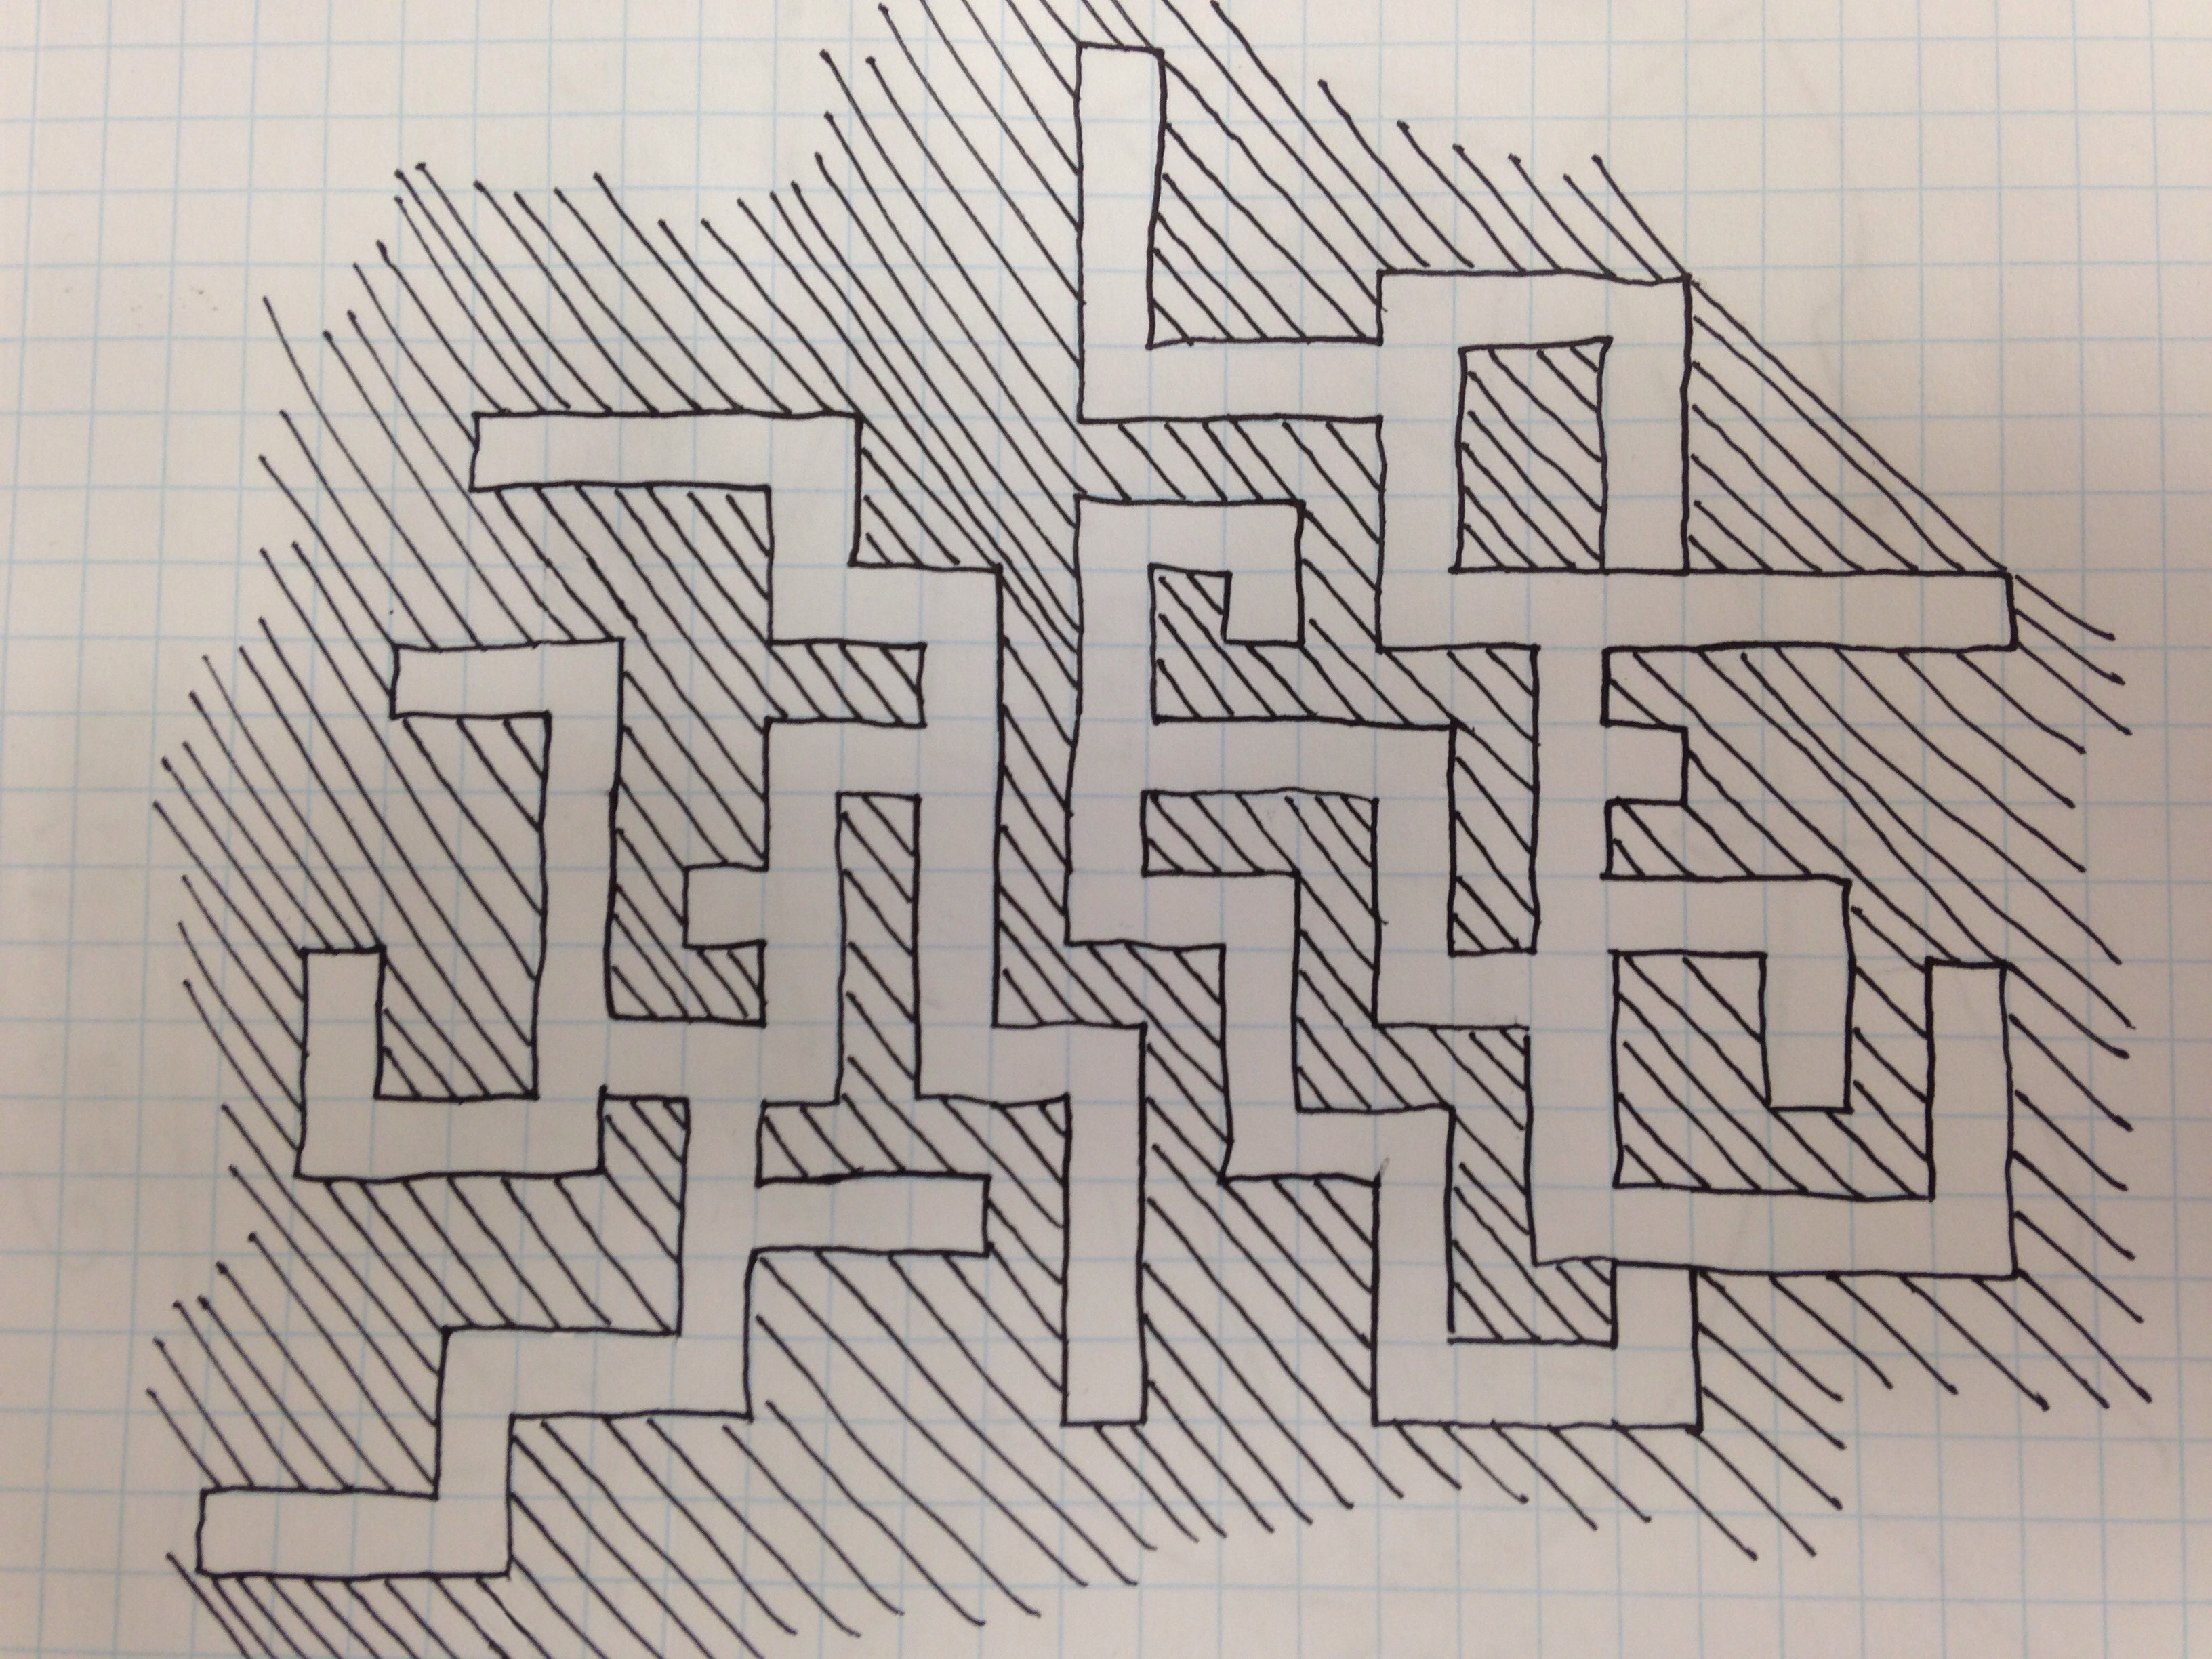
\includegraphics[width=0.75\linewidth]{img/maps/HONE.png} 
	
	{\textbf{Aethereu:} The Halls of no end is a puzzle area. There is one exit and it's the dead end which appears on the 2 long hallway to the left. Each hallway continues onto the hallway that is of the same length but opposite direction as it. The dead end is a perfectly flat wall like all others in this place with nine and three-quarter dashes on the top side of the wall. This is a reference to Harry potter and the wall can be entered with a slight jog. This zone was created by Baba.}
\end{center}

\subsection{Yaga}

\begin{commentbox}{Kharazan}
	Kharazan is a tower that is about a 3 days journey to the northeast of Aurushire. Kharazan is a huge but semi-deserted castle. The place is old and many parts of it are broken down. There are many rooms in it such as a ballroom, full storehouse, large dining halls, dungeons, libraries, theaters, etc (Modeled similarly to the Kharazan castle in World of Warcraft). This place is where Yaga resides deep into one of the libraries of the castle up in one of the highest castles. Most of the things found within the castle are dust covered and appear to have not been used in many years.
	
	At the entrance of the castle lies a sleeping curator. This is a robotic like creature (very large) that will awaken if anyone enters the place. This curator is not hostile unless provoked or protecting the castle. This curator serves the master of the castle and can be used to give information or lead the party to where they need to go. Throughout the castle, there is a faint tune playing continually that is caused by an enchantress' spell created after the castle was abandoned.
\end{commentbox}

\begin{center}
	\includegraphics[width=0.5\linewidth]{img/Yaga.jpg} \includegraphics[width=0.43\linewidth]{img/ed94712ddd2dfc1bcc41918c9bda155e.jpg}
\end{center}

\begin{monsterbox}{Yaga}
	\begin{hangingpar}
		\textit{?? ??, Neutral ??}
	\end{hangingpar}
	\dndline%
	\basics[%
	armorclass = ??,
	hitpoints  = ??,
	speed      = ?? ft
	]
	\dndline%
	\stats[
	STR = \stat{}, % This stat command will autocomplete the modifier for you
	DEX = \stat{},
	CON = \stat{},
	INT = \stat{},
	WIS = \stat{},
	CHA = \stat{}
	]
	\dndline%
	\details[%
	% If you want to use commas in these sections, enclose the
	% description in braces.
	% I'm so sorry.
	languages = {Common},
	challenge = 20
	]
	\dndline%
	\monstersection{Description/Information}
	Yaga is an old sorcerer. Not much is known about her. She is tall and frail (or at least appears so). It is impossible to tell anything about her from looking at her. This NPC is a wild card. It can be used with the story as seen fit (save the important things she contains to the campaign).
\end{monsterbox}

\begin{commentbox}{The Ying-Yang}
	The Ying-Yang (Baba and Yaga) plays an important part of this campaign. 
	
	Baba is a wizard that is interested in helping the party learn. She contains a vast library of knowledge and knows much about the Trinity stone legends and myths. She can assist the party in learning more. Similarly, she will insist the party is not ready if they claim they are seeking Athereu and if they insist they are will put the party through tests to confirm it. One test is to teleport the party to the halls of no end. Another would be to send them into Rem Silva after something that would help them on their journey. These challenges would be designed to assist them in their journey. 
	
	Yaga is an old witch. She appears to contain vast knowledge of the trinity stone legends as well, but acts as if she knows nothing. She can assist the party in acquiring clues and items that will help find their way to their goal. Specifically, she contains a map of Aethereu (the inside) which appears as a blank piece of paper until entering Aethereu. This map is pivotal to easily navigating the chamber. Alternatively, she can contain clues regarding successful passage through The Pluvian Forest, along with Baba.
\end{commentbox}



\begin{commentbox}{Samilah}
	Samilah, which is a name derived from Samson and Delilah meaning ``shining night''. She can be placed into the campaign in many ways but serves as the mortal embodiment of the Celestials. Her main goal is to destroy the San'graal which is the only mortal weapon known to be able to destroy the Celestials. She can disguise herself as any other sentient being and has a necklace that will protect her from any harm. She is mentally disciplined so that her mind cannot be messed with and has nearly unlimited capabilities. After destroying the San'graal she will lead the Celestial army in the conquest of Orilla.
	\begin{center}
		\includegraphics[width=0.675\linewidth]{img/samilah.jpg} \includegraphics[width=0.29\linewidth]{img/Adria_Ark_of_Truth.jpg}
	\end{center}
\end{commentbox}

\subsection{The Eternal Neokoros}

\begin{commentbox}{Eternal Neokoros}	
	The Eternal Neokoros is a creature modeled after the Eternal Neokoros from the Halo series. It's appearance and voice mirror that of the Halo creature but it's purpose is expanded for use in this campaign. This creature has existed since before humanity. It lives deep in the Earth and prefers warm and humid climates. The creature is not very mobile as far as relocating its self, however it is extremely agile in battles as it has a large amount of tendrils that can poison, paralyze, attack and more to anything it desires. The creature typically travels through a cave system that exists on volcanic fault lines under oceans. 
	
	Where the creature can appear in the campaign can vary but is typically if a player, or the party finds themselves adrift in the ocean or body of water. The creature needs a large amount of time to surface and show itself. It can also extend its tendrils vast distances and could collect objects or people from long distances away (such as under a body of water). It does need a large amount of time to do this so the target would need to be immobilized or inanimate. The Eternal Neokoros is well aware of most things occurring on the surface of the planet as it can hear through rock and metal and continually watches and learns as the species of the planet develop. The Eternal Neokoros has rarely been seen throughout history but some Legends and stories have arose from it such as that of the Loch'Ness Monster and that of a flood invasion.
	
	\begin{center}
		\includegraphics[width=0.95\linewidth]{img/Halo/gravemind.jpg}
	\end{center}

	The Eternal Neokoros can create an offspring Neokoros within a host creature. The offspring has a faint link to the Eternal Neokoros and shares an eternal bond that links the creatures through space. If the offspring of the Eternal Neokoros is killed by a sentient being, the Eternal Neokoros will feel the pain of losing its child and seek revenge.
\end{commentbox}

\begin{monsterbox}{Eternal Neokoros}
	\begin{hangingpar}
		\textit{Huge Huge Monstrosity, Chaotic Neutral}
	\end{hangingpar}
	\dndline%
	\basics[%
	armorclass = 22 (Body) + 25 (tendrils),
	hitpoints  = 460,
	speed      = 5 ft (self) + 50 ft (tendrils)
	]
	\dndline%
	\stats[
	STR = \stat{21}, % This stat command will autocomplete the modifier for you
	DEX = \stat{18},
	CON = \stat{30},
	INT = \stat{30},
	WIS = \stat{24},
	CHA = \stat{16}
	]
	\dndline%
	\begin{monsteraction}[Eternal Wisdom]
		The eternal nature of this beast gives it infinite capabilities with mental challenges. The creature cannot fail wisdom checks/saves.
	\end{monsteraction}	
	\begin{monsteraction}[Legendary Action]
		If the eternal creature fails a saving throw, it can instead choose to succeed. This can occur up to 2 times a day.
	\end{monsteraction}
	\begin{monsteraction}[Unpredictable Tendril Presence]
		Because of the number of tendrils and size of the creature, it gets four separate turns in the initiative order. One for the Eternal Neokoros and three for each major tendril. 
	\end{monsteraction}	
	\begin{monsteraction}[Eternal Horror]
		The creature appears extremely horrifying and terrifying. Any creature seeing it must make a DC18 constitution save. If the target fails it is frightened and cannot take actions until an action is taken against them. 
	\end{monsteraction}	
	
	\monstersection{Actions}
	\begin{monsteraction}[Eternal Attack Pattern]
		The creature is so intelligent that it can manipulate all of it's tendrils in a precise manner and coordinate attacks flawlessly. Because of this it can take 3 attacks or actions per turn.
	\end{monsteraction}
	\begin{monsteraction}[Eternal Whip]
		The creature can whip a tendril towards a target. +9 hit and deals 4d6 damage. This will also paralyze any target that is grappled.
	\end{monsteraction}
	\begin{monsteraction}[Eternal Bind]
		\begin{itemize}
			\item The creature can burrow one of it's tendrils through the ground and wrap itself around a player without them realizing. The tendril can then pull the target's leg into the ground (except through rock or metal) causing the target to be grappled by the ground.
			\item Alternatively, the creature can grapple a being with one of its tendrils.
		\end{itemize}
	\end{monsteraction}
	\begin{monsteraction}[Paralytic Substance]
		The creature can excrete a goo-like compound from any of it's tendrils that can paralyze an opponent. 
	\end{monsteraction}
	\begin{monsteraction}[Throw Creature]
		If a target is grappled by one of the creatures tendrils, it can throw the target causing 3d10+4 damage.
	\end{monsteraction}
	\begin{monsteraction}[Eternal Deafening]
		The creature can use an action to impose a psychic attack on every foe it's facing simultaneously. All creatures must make a DC 18 Wisdom save. On a succeed, they obtain a headache and a nose bleed and take 2 damage. On a fail, they also take 1d8 damage.
	\end{monsteraction}
	
	\details[%
	% If you want to use commas in these sections, enclose the
	% description in braces.
	% I'm so sorry.
	languages = {All},
	challenge = 20
	]
	\dndline%
	\monstersection{Description/Information}
	The Eternal Neokoros can only be seen by killing the Neokoros offspring, thus provoking revenge. This creature is extremely large and essentially requires an army to defeat.	
		
	\begin{center}
		\includegraphics[width=0.5\linewidth]{img/Halo/gravemind-battle.jpg} \includegraphics[width=0.485\linewidth]{img/Halo/gravemind-face.jpg}
	\end{center}
\end{monsterbox}

\begin{monsterbox}{Neokoros Tendril}
	\begin{hangingpar}
		\textit{Huge Huge Monstrosity, Chaotic Neutral}
	\end{hangingpar}
	\dndline%
	\basics[%
	armorclass = 21 (Body) + 23 (tendrils),
	hitpoints  = 180,
	speed      = 5 ft (self) + 40 ft (tendrils)
	]
	\dndline%
	\stats[
	STR = \stat{21}, % This stat command will autocomplete the modifier for you
	DEX = \stat{18},
	CON = \stat{30},
	INT = \stat{30},
	WIS = \stat{24},
	CHA = \stat{16}
	]
	\dndline%
	\begin{monsteraction}[Eternal Connection]
		The Tendril has all of the same abilities as the Eternal Neokoros as it is attached to it.
	\end{monsteraction}	
	
	\monstersection{Actions}
	\begin{monsteraction}[Eternal Devour]
		If a creature is close to the tendril, it can open up with multiple layers of teeth and attempt to devour a creature. The creature must make a DC16 dexterity saving throw or take 3d6+4 damage. If this kills the target, they are devoured and instantly gain three failed death saves.
	\end{monsteraction}
	\begin{monsteraction}[Eternal Whip]
		The creature can whip a tendril towards a target. +8 hit and deals 4d6 damage. This will also paralyze any target that is grappled.
	\end{monsteraction}
	\begin{monsteraction}[Eternal Bind]
		\begin{itemize}
			\item The creature can burrow one of it's tendrils through the ground and wrap itself around a player without them realizing. The tendril can then pull the target's leg into the ground (except through rock or metal) causing the target to be grappled by the ground.
			\item Alternatively, the creature can grapple a being with one of its tendrils.
		\end{itemize}
	\end{monsteraction}
	\begin{monsteraction}[Paralytic Substance]
		The creature can excrete a goo-like compound from any of it's tendrils that can paralyze an opponent. 
	\end{monsteraction}
	\begin{monsteraction}[Throw Creature]
		If a target is grappled by one of the creatures tendrils, it can throw the target causing 3d10+4 damage.
	\end{monsteraction}
	\begin{monsteraction}[Eternal Deafening]
		The creature can use an action to impose a psychic attack on every foe it's facing simultaneously. All creatures must make a DC 18 Wisdom save. On a succeed, they obtain a headache and a nose bleed and take 2 damage. On a fail, they also take 1d8 damage.
	\end{monsteraction}
	
	\details[%
	% If you want to use commas in these sections, enclose the
	% description in braces.
	% I'm so sorry.
	languages = {All},
	challenge = 15
	]
	\dndline%
	\monstersection{Description/Information}
	The Eternal Neokoros Tendril appears when the Eternal Neokoros is around. This is a major Tendril connected to the Eternal Neokoros which has it's own set of tendrils that send out attacks.
\end{monsterbox}

\begin{commentbox}{Neokoros}
	The Eternal Neokoros can lay an offspring by intertwining a bit of its DNA into another creatures nervous system. The offspring is known as Neokoros and grows in strength as the player grows. This offspring can act on it's own and becomes part of its host (similar to Venom from the spider-man series). As time passes, it can develop a relationship with the host or overtake them. Instead of having it's own turn order and stats, it instead increases the stats of a player when active. The creature can activate when it desires. If the player has a relationship with the creature, it can have some influence on when the creatures abilities activate. The main purpose of the creature is to do whatever the Eternal Neokoros gave it as its mission. For the purposes of this campaign, it's mission is to find the Trinity Stones and destroy the Celestials, though it doesn't know this precisely until the creature grows and develops more. The consciousness of the creature will slowly unravel over time.
	
	The appearance of the Neokoros can vary greatly. One method of such appearance is to appear as an alien eye within the host. The eye would have small purple veins that were not there before the infection that stem from the eye on the side of the hosts head. The parasite cannot be removed without killing the host player. Abilities of the Neokoros are determined by the level of the host creature.
	
	The Neokoros can heal the player for 1d6 per host level at any point it chooses. This can occur once per long rest. The creature also gains the following abilities and all abilities of lower levels.
	
	\begin{description}
		\item[Level 1:] The creature can telepathically communicate with the player, occasionally speaking single words or phrases.
		\item[Level 2:] The creature can sometimes move the host when the host is unconscious.
		\item[Level 3:] The creature can sometimes provide a strength success when the host is acting with their reflexes. 
		\item[Level 4:] The creature can sometimes provide an increase in combat abilities of the player.
		\item[Level 5:] The creature begins to communicate more with the host alerting the host that it has a conscious.
		\item[Level 6:] The creature can sometimes control the player while the player is conscious.
		\item[Level 7:] The creature can create visual hallucinations for the player.
		\item[Level 8:] The creature will try to either manipulate or befriend the host.
		\item[Level 9:] The creature provides a permanent +1 to strength to the host as it begins to alter the host internal cellular structure.
		\item[Level 10:] The creature can provide intelligence and combat bonuses for the player when it desires. 
 	\end{description}
\end{commentbox}




\chapter{Extended Campaign and Universe}

\section{Old Gods}

The old gods exist prior to the Celestials and well known gods of the world. These gods have an origin that could be from any point in history and from any place in history far before the existence of modern life on Orilla. These gods were of the first ascended beings in the universe. the Old gods of Orilla have lived for what could be seen as eternity and have long since decided to slumber and not interact with the mortal realm. Their power and abilities are far superior to any other beings in the universe and even as they slumber they can still greatly influence the mortal realms and even that of the ascended beings (modern gods).

\subsection{Yogg'Saron}

Yogg'Saron\footnote{Modeled after Yogg'Saron from World of Warcraft.} is an old god based on insanity. Yogg'Saron has been slumbering for the entire entire existence of life on Orilla. Even though he has been slumbering, his influence is so great that some creatures in the past have been driven insane by his mental influence and became servants embodying his essence in physical form. These servants have caused destruction and chaos throughout ancient times and left remnants of power that can still be found today. 

Yogg'Saron's most powerful influence was through a great beast that is believed by many to have been the entire essence of Yogg. The beast was vanquished by an army of highly trained soldiers with the help of a demigod Ursoc, whom described him as ``the beast with a thousand maws.'' The beast had such a strong influence from Yogg, that the blood of the creature was used for forging great and powerful items following the beasts defeat. Unfortunately, as the blood was also influenced by Yogg, the items created with the beasts blood have an inherent connection to Yogg.

\begin{center}
	\includegraphics[width=\linewidth]{img/WoW/yogg-saron.jpg}
\end{center}

Yogg'Sarons existence is believed to be unknown to most of the inhabitants of Orilla. However, Yogg's power is so vast that the maddening, destructive taint seeps from its resting place and appears to tear at the sanity of an unknown number of Orilla's inhabitants. Because of this, Yogg possess worshipers across all the world's peoples and cultures.

\subsubsection{Yogg'Saron Puzzle Box}

The Yogg'Saron puzzle box\footnote{From https://wowwiki.fandom.com/wiki/Puzzle\_Box\_of\_Yogg-Saron} is an artifact that was created with a connection to Yogg'Saron. The box is magically sealed and contains many shifting panels, hidden hinges, changing sides, magical barriers and more. The box is made of an allow of hardened Yogg'Saron blood and a substance called Katchin\footnote{Katchin from Dragonball Z.}, which is one of the hardest materials in the universe. The box is indestructible and appears impossible to actually solve and open. When attempting to open the box, the box will whisper messages to you to try and drive the user to insanity. 

\begin{multicols}{2}
	\begin{itemize}
		\item At the bottom of the ocean even light must die
		\item The silent, sleeping, staring houses in the backwoods always dream. It would be merciful to tear them down.
		\item There is no sharp distinction between the real and the unreal.
		\item Even death may die.
		\item There is a little lamb lost in dark woods.
		\item All places, all things have souls. All souls can be devoured.
		\item What can change the nature of a man?
		\item The stars sweep chill currents that make men shiver in the dark.
		\item You will all be alone in the end.
		\item Do you dream while you sleep or is it an escape from the horrors of reality?
		\item Look around. They will all betray you. Flee screaming into the black forest.
		\item In the land of Ny'alotha there is only sleep.
		\item In the sleeping city of Ny'alotha walk only mad things.
		\item Ny'alotha is a city of old, terrible, unnumbered crimes.
		\item Y'knath k'th'rygg k'yi mrr'ungha gr'mula.
		\item The void sucks at your soul. It is content to feast slowly.
		\item The drowned god's heart is black ice.
		\item It is standing right behind you. Do not move. Do not breathe.
		\item Have you had the dream again? A black goat with seven eyes that watches from the outside.
		\item In the sunken city, he lays dreaming.
		\item Open me! Open me! Open me! Then only will you know peace.
		\item You resist. You cling to your life as if it actually matters. You will learn.
		\item The tortured spirits of your ancestors cling to you, screaming in silence. Apparently they are quite numerous.
		\item The fish know all the secrets. They know the cold. They know the dark.
		\item The giant rook watches from the dead trees. Nothing breathes beneath his shadow.
		\item Beneath the shadow of the darkened spire, there is no light, no mercy, only void, and the chaos within. 
		\item They are coming for you...
		\item Give in to your fear...
		\item Kill them all... before they kill you...
		\item They have turned against you... now, take your revenge...
		\item It WAS your fault...
		\item Tell yourself again that these are not truly your friends...
		\item You are a pawn of forces unseen...
		\item There is no escape... not in this life... not in the next... 
		\item Trust is your weakness...
		\item Hope is an illusion...
		\item All that you know will fade...
		\item You will be alone in the end... 
	\end{itemize}
\end{multicols}



\chapter{The Zones}

\section{The Statu Peninsula}

The Statu peninsula (commonly referred to as just Statu) is largely un-mapped area. As the name suggests, Statu is a peninsula that cannot be accessed from foot to the north. It contains very dense forestation and mountainous regions to the northern area that are not possible to travel through. The south is colonized by Aurushire where a small number of people settle. There are generally a small number of visitors to Statu, save those who are trading and working with the mines to the East of Aurushire. The best way to access Statu is through the Aurushire port.

To the West of Aurushire, there is a large forest that is significantly less dense than the northern regions. To the north of this is very dense un-explored forest and mountainous regions. Directly north of Aurushire is The Pluvian Forest. This region is not very often visited. Strange occurrences pertaining to what some call 'strange spatial events' occur in The Pluvian Forest which generally ward off visitors. To the east of Aurushire, there is a hostile tribe of river Naga which attack travelers and visitors on sight. Because of this, the area to the east and the forest regions to the east of Aurushire are largely unexplored. What is known of this region is that there is a large valley that leads from the Naga camps into the mountain/forest region. These are just north of the shore.

Also to the East of Aurushire is a large shoreline that extends a few days journey. The shore is boundaries by the ocean and sharp mountainous rock faces that are virtually unclimbable. The shore directly to the east of Aurushire is a very shallow and rocky region for a few miles. This region has regions where the mud has undergone chemical reactions over time to become firm and hard much like concrete. This makes the region semi-easy to travel through with the only challenge being the shallow water covering the entire region. Directly to the east of this area is marsh and swamplands that extend for another 40-50 or so miles. This takes about 2-3 days to journey through. Continuing further, as the marsh levels off, there is a dense region of Jungle that is nearly untouched by people due to the danger it poses to travelers. Even further east is sheer rock face and not traversable. The marsh area is covered by a thick fog that makes it hard to see anything and is home to a vast amount of creatures. All three coastal regions are surrounded by huge rock faces.

\section{Aurushire}

Aurushire (also commonly referred to as Goldshire) is a small village located on the southern end of the Statu peninsula. Just East of Aurushire is a large mountain containing mine shafts used for gold mining. It is not well known, other by those who work in the mines, but strange things happen within these mines where mined gold will spontaneously be regrown after being removed from the mines. This phenomenon is where Aurushire (Goldshire) retreived its name from and is thought to be related to the spacial occurrences reported in The Pluvian Forest. 

\subsection{NPC's}

Aurushire is full of NPC characters. Many of them are just normal workers or village folk, however some serve an important purposes. Some of them include the innkeeper, the Pandaren Brothers, the village watchers and the shopkeepers.

\begin{monsterbox}{Arryn}
	\begin{hangingpar}
		\textit{Halfling Wizard, Neutral Good}
	\end{hangingpar}
	\dndline%
	\basics[%
	armorclass = 17,
	hitpoints  = 172,
	speed      = 40 ft
	]
	\dndline%
	\stats[
	STR = \stat{12}, % This stat command will autocomplete the modifier for you
	DEX = \stat{12},
	CON = \stat{16},
	INT = \stat{20},
	WIS = \stat{18},
	CHA = \stat{18}
	]
	\dndline%
	\details[%
	% If you want to use commas in these sections, enclose the
	% description in braces.
	% I'm so sorry.
	languages = {Common, Elvish, Dwarvish, Gnomish, Halfling, Orc, Pandaren},
	challenge = 10
	]
	\dndline%
	\begin{monsteraction}[Mystical Senses]
		If a target tries to deceive you, it must make a DC19 deception saving throw.
	\end{monsteraction}	
	\begin{monsteraction}[Water sight]
		You can see clearly up to two miles over water.
	\end{monsteraction}
	\monstersection{Actions}
	\begin{monsteraction}[Bladesinger: Extra Attack]
		You can attack twice on your turn.
	\end{monsteraction}
	\begin{monsteraction}[Hold Monster]
		A creature you can see within 90 feet must succeed on a wisdom saving throw or be paralyzed for 1 minute. Target can make a wisdom saving throw at the end of each of it's turns to end the spell.
	\end{monsteraction}
	\begin{monsteraction}[Magic Jar Master]
		Allows Arryn to use Magic Jar on a nearby jar instantly and without being in a jar himself.
	\end{monsteraction}
	\begin{monsteraction}[Magic Jar]
		Long description, look it up.
	\end{monsteraction}
	\monstersection{Description/Information}
	Arryn is the first NPC most encounter when entering Aurushire from sea. He is the watcher of the ports and lives on a small farm right at docks where all sea traffic enters from.
\end{monsterbox}

\begin{center}
	\includegraphics[width=0.7\linewidth]{img/chen.jpg}
\end{center}

\begin{monsterbox}{Chen Stormstout}
	\begin{hangingpar}
		\textit{Pandaren Monk, Neutral Good}
	\end{hangingpar}
	\dndline%
	\basics[%
	armorclass = 17,
	hitpoints  = 172,
	speed      = 40 ft
	]
	\dndline%
	\stats[
	STR = \stat{18}, % This stat command will autocomplete the modifier for you
	DEX = \stat{20},
	CON = \stat{16},
	INT = \stat{12},
	WIS = \stat{12},
	CHA = \stat{18}
	]
	\dndline%
	\details[%
	% If you want to use commas in these sections, enclose the
	% description in braces.
	% I'm so sorry.
	languages = {Common, Elvish, Dwarvish, Gnomish, Halfling, Orc, Pandaren},
	challenge = 10
	]
	\dndline%
	\begin{monsteraction}[Joint lock]
		You can put a creature in a joint lock when attacking. Remove 1d6 damage from the attack and instead roll 1d20 to decide on how severe the joint lock is. 
		
		1-3: The joint lock fails. 
		
		4-14: You pop a joint briefly out of place causing the enemy to have disadvantage on their next attack.
		
		15-19: You dislocate the targeted limb, causing the opponent to not be able to use it until set (which can be done via an action on their turn). You can choose to roll less if desired.
		
		20: You tear the tendons holding a limb on, causing it to become useless until healed. You can choose to roll less if desired.
	\end{monsteraction}
	\begin{monsteraction}[Pressure Point Mastery]
		You can target a creatures pressure points when attacking. Remove 1d6 damage from the attack and instead roll 1d20 to decide how accurate the points are hit. 
		
		1-3: The pressure points fail. 
		
		4-14: You hit a target in a precious spot causing them great discomfort. They must roll attack rolls at disadvantage next round.
		
		15-19: The target becomes stunned for one round of combat. You can choose to roll less if desired.
		
		20: The target becomes completely paralyzed. You can choose to roll less if desired.
	\end{monsteraction}
	\monstersection{Actions}
	\begin{monsteraction}[Pandaren Nimbleness: Extra Attack]
		You can attack twice on your turn.
	\end{monsteraction}
	\begin{monsteraction}[Melee]
	This is a normal un-armed melee attack: +6 to hit. Deals 3d6 +5 damage.
	\end{monsteraction}
	\begin{monsteraction}[Armed Melee]
		This is a normal melee attack using a weapon. Depending on the weapon, it can add damage to the Melee attack. Spear/staff: +6 damage, Sword: +4 damage, Hammer/Axe: +2 damage.
	\end{monsteraction}

	\monstersection{Description/Information}
	Chen Stormstout runs the Aurushire Pub. He spends his time wandering the nearby regions for herbs and ingredients to make the perfect brews. He also studies martial arts with his brothers. He focuses on pressure points and joint locks and studies a more fluid form of combat.
\end{monsterbox}

\begin{center}
	\includegraphics[width=0.7\linewidth]{img/ekron.jpg}
\end{center}

\begin{monsterbox}{Ekron Stormstout}
	\begin{hangingpar}
		\textit{Pandaren Barbarian, Neutral Good}
	\end{hangingpar}
	\dndline%
	\basics[%
	armorclass = 17,
	hitpoints  = 172,
	speed      = 50 ft
	]
	\dndline%
	\stats[
	STR = \stat{20}, % This stat command will autocomplete the modifier for you
	DEX = \stat{18},
	CON = \stat{18},
	INT = \stat{12},
	WIS = \stat{12},
	CHA = \stat{16}
	]
	\dndline%
	\details[%
	% If you want to use commas in these sections, enclose the
	% description in braces.
	% I'm so sorry.
	languages = {Common, Elvish, Dwarvish, Gnomish, Halfling, Orc, Pandaren},
	challenge = 10
	]
	\dndline%
	\begin{monsteraction}[Fury of Blows]
		If you have two swords, you can furiously attack your opponent without them being able to block. You can sacrifice any number of 1d6's from the attack roll to destroy an item the opponent has on them.
	\end{monsteraction}	
	\monstersection{Actions}
	\begin{monsteraction}[Pandaren Nimbleness: Extra Attack]
		You can attack twice on your turn.
	\end{monsteraction}
	\begin{monsteraction}[Melee]
	This is a normal un-armed melee attack: +6 to hit. Deals 3d6 +5 damage.
	\end{monsteraction}
	\begin{monsteraction}[Armed Melee]
		This is a normal melee attack using a weapon. Depending on the weapon, it can add damage to the Melee attack. Spear/staff: +4 damage, Sword: +6 damage, Hammer/Axe: +2 damage.
	\end{monsteraction}
	\monstersection{Description/Information}
	Ekron, like his brothers, also studies martial arts.He focuses on agility and movements to quickly take down his opponents with a fierce and fast form of combat. He is the keeper of the Aurushire Quarries and leads the mining operations. He found a small panda in the forest one day and has been cherishing it ever since as a friend and companion.
\end{monsterbox}

\begin{center}
	\includegraphics[width=0.7\linewidth]{img/mishnah.jpg}
\end{center}

\begin{monsterbox}{Mishnah Stormstout}
	\begin{hangingpar}
		\textit{Pandaren, Neutral Good}
	\end{hangingpar}
	\dndline%
	\basics[%
	armorclass = 17,
	hitpoints  = 172,
	speed      = 30 ft
	]
	\dndline%
	\stats[
	STR = \stat{20}, % This stat command will autocomplete the modifier for you
	DEX = \stat{18},
	CON = \stat{18},
	INT = \stat{12},
	WIS = \stat{16},
	CHA = \stat{18}
	]
	\dndline%
	\details[%
	% If you want to use commas in these sections, enclose the
	% description in braces.
	% I'm so sorry.
	languages = {Common, Elvish, Dwarvish, Gnomish, Halfling, Orc, Pandaren},
	challenge = 10
	]
	\dndline%
	\begin{monsteraction}[Thunderous Blow]
		You can sacrifice 2d6 on an attack roll to instead deal 1d4 thunderous damage to all enemies within 15 feet of the blow you deal.
	\end{monsteraction}	
	\monstersection{Actions}
	\begin{monsteraction}[Pandaren Nimbleness: Extra Attack]
		You can attack twice on your turn.
	\end{monsteraction}
	\begin{monsteraction}[Melee]
		This is a normal un-armed melee attack: +6 to hit. Deals 3d6 +5 damage.
	\end{monsteraction}
	\begin{monsteraction}[Armed Melee]
		This is a normal melee attack using a weapon. Depending on the weapon, it can add damage to the Melee attack. Spear/staff: +2 damage, Sword: +4 damage, Hammer/Axe: +6 damage.
	\end{monsteraction}
	\monstersection{Description/Information}
	Mishnah Stormstout is the Aurushire Blacksmith. He spends his time collecting rocks and forging precious metals found in his brothers mine. He also studies martial arts but tends more towards a body building focus and overpowers his foes through brute strength.
\end{monsterbox}

\begin{center}
	\includegraphics[width=0.7\linewidth]{img/bob.jpg}
\end{center}

\begin{monsterbox}{Bob}
	\begin{hangingpar}
		\textit{Orcish Barbarian, Neutral Good}
	\end{hangingpar}
	\dndline%
	\basics[%
	armorclass = 17,
	hitpoints  = 151,
	speed      = 30 ft
	]
	\dndline%
	\stats[
	STR = \stat{20}, % This stat command will autocomplete the modifier for you
	DEX = \stat{18},
	CON = \stat{17},
	INT = \stat{16},
	WIS = \stat{15},
	CHA = \stat{13}
	]
	\dndline%
	\details[%
	% If you want to use commas in these sections, enclose the
	% description in braces.
	% I'm so sorry.
	languages = {Common, Dwarvish, Orc},
	challenge = 9
	]
	\dndline%
	\begin{monsteraction}[Experienced Pain]
		Bob has seen some things. He can ignore any major wounds or hindrances that would effect his combat. He can fight full power until his last breath. This is due to his combat experience and many near death experiences.
	\end{monsteraction}	
	\begin{monsteraction}[Battle Master]
		Bob can quickly pick up and adapt to using most weapons, gaining proficiency with any new weapons after using them.
	\end{monsteraction}	
	\monstersection{Actions}
	\begin{monsteraction}[Combat experience: Extra Attack]
		You can attack twice on your turn.
	\end{monsteraction}
	\begin{monsteraction}[Melee]
		This is a normal un-armed melee attack: +6 to hit. Deals 2d6 +5 damage.
	\end{monsteraction}
	\begin{monsteraction}[Throwing Axe]
		Bob carries 4 throwing axes that he can hurl towards an enemy. +5 to hit. 3d6 +2 damage. Range: 40 ft.
	\end{monsteraction}
	\monstersection{Description/Information}
	
\end{monsterbox}


\subsection{The Inn of the Prancing Pony}

This is the inn located in Aurushire. The innkeeper is named Artemisia who is kind of like the grandmother of the small village. 

\subsection{Tracey's Armory}

Tracey's Armory is the armor shop in Aurushire. The shopkeeper is Tiberias Tracey, who is one of the great grandchildren of the original shop's builder. This shop contains simple and custom armor pieces that are created for all who are willing to pay or friends of Tiberias. 

\subsection{Bob's Guns}

Bob's Guns is a relatively newly built shop. The majority of what is sold here is ranged weapons. Due to the effects of the Pluvian Forest, Bob (the storekeeper) discovered a weapon laying in the wild on someones corpse. He was able t reverse engineer approximately how it worked and has been creating 'guns' ever since. Unfortunately he used all of the bullets on the original design, but he was able to examine the weapon itself and deduce a process to recreate a similar mechanism, His own designs are not as well made as the original discovery, but they are slowly improving over time. Bob also sells spears, throwing stars, darts, bows and more.

\subsection{Stormstout Blacksmith}

This is the village blacksmith that is run by one of the Stormstout brothers (Mishnah). The blacksmith is one of the watchers of the village and most influential members. Mishnah is also friends with everyone else in the village and generally his services are needed by almost all of the members.

\subsection{Stormstout Pub}

This is the village brewery which is unlike any brewery anywhere else. The brewery is run by one of the Stormstout brothers (Chen). Chen ha ssome of the most unique brews of anywhere else in Orilla. This is primarily due to the ingredients and herbs that he has found throughout the nearby forests. Chen is one of the friendliest people in Aurushire and most people go to him with their issues or thoughts. He is generally a sociable person and many people hang out at his Brewery/Pub in their free time. Chen is also one of the watchers of the village and most influential members.

\subsection{Stormstout Quarries}

The Stormstout Quarries are the mines that reside to the East of Aurushire. The mines are run by one of the Stormstout brothers (Ekron). Ekron is a strong military leader and one of the most influential members of Aurushire. The mines are known for their unique regrowth of some of the ores within them. It is believed that these occurrences are as a result of effects on the region by the Pluvian Forest. The quarries will pay any willing workers with a part of their earnings. Ekron is one of the watchers of the village.

\subsection{Library of Lysanias}

The village has a library that is open to all. There are a number of people who spend a lot of time here and maintain it but for the most part it is open and there is no main keeper. The library is public and contains mostly learning material and books written by previous and past villagers.

\section{Rem Silva}

Rem Silvia is the name of the Forest that is located to the West of Aurushire. This forest, along with The Pluvian Forest often experiences strange spacial phenomenon. Unlike The Pluvian Forest, temporal phenomenon have also commonly been reported as occurring in this region. The occurrences of these random phenomenon do not appear marginally as often or as strong as in The Pluvian Forest which makes this region of particular interest to experienced hunters.

The same strange effects that can occur in the Pluvian forest can also occur here in Rem Silva only less frequently. As a DM, you can periodically roll a 1d20 to see if any of the irregular effects from The Pluvian Forest will also occur here. Subtract 5 from each DC throw to see if the effects occur in this region.

This area is full of a large number of creatures, from large spiders, to night elfs. Due to the trinity stone effects, many creatures not belonging to this region also appear here. 

\begin{center}
	\includegraphics[width=\linewidth]{img/maps/RemSilva.png}
	
	{\textbf{Rem Silva:} A forest to the west of Aurushire. To the north/Northeast is The Pluvian Forest but the forest is too dense to travel between the two.}
\end{center}

\begin{commentbox}{Random Encounters}
	At any time, a party traveling through this area could run into a creature. To determine a random encounter you can roll 1d100 and choose what the party will encounter. If the roll is odd, choose a miscellaneous creature from Appendix A of the monster manual (page 317-337 in monster manual, roll 1d20 to decide page of creature to choose), otherwise if the roll is even, choose from the table below. Similarly, Page 97 of Xanathars may be useful for creating random encounters.
	\begin{description}
		\item[1-10:] Displacer Beast
		\item[11-20:] Basilisk
		\item[21-25:] Dinosaur (page 79-80 of monster manual)
		\item[26-30:] Unicorn (page 294 of monster manual)
		\item[31-40:] Night elf(s)
		\item[41-45:] Ettin (page 132 of monster manual)
		\item[46-50:] troll (page 291 of monster manual)
		\item[51-55:] Galeb Duhr (page 139 of monster manual)
		\item[56-60:] Yeti (page 305 of monster manual)
		\item[61-65:] Ghost (page 147 of monster manual)
		\item[66-70:] Hook Horrer (page 189 of monster manual)
		\item[71-75:] Griffon (page 174 of monster manual)
		\item[76-80:] Hippogriff (page 184 of monster manual)
		\item[81-85:] Hell Hound (page 182 of monster manual)
		\item[86-90:] Jackalwere (page 193 of monster manual)
		\item[91-95:] Homunculus (page 188 of monster manual)
		\item[96-99:] Treant (page 289 of monster manual)
		\item[100:] Mythical Beast
	\end{description}
\end{commentbox}

\subsection{NPC's/Modified Creatures}

\begin{center}
	\includegraphics[width=0.38\linewidth]{img/WoW/Rexxar2.png}
	\includegraphics[width=0.6\linewidth]{img/WoW/Rex.jpg}
\end{center}
\begin{monsterbox}{Rexxar}
	\begin{hangingpar}
		\textit{Large humanoid, unaligned}
	\end{hangingpar}
	\dndline%
	\basics[%
	armorclass = 21,
	hitpoints  = 457,
	speed      = 50 ft
	]
	\dndline%
	\stats[
	STR = \stat{27}, % This stat command will autocomplete the modifier for you
	DEX = \stat{14},
	CON = \stat{25},
	INT = \stat{16},
	WIS = \stat{15},
	CHA = \stat{19}
	]
	\dndline%
	\details[%
	% If you want to use commas in these sections, enclose the
	% description in braces.
	% I'm so sorry.
	savingthrows = {Dex +9, Con +14, Wis +9, Char +11},
	skills = {Perception +16, Stealth +9},
	senses = {darkvision 90 ft., passive perception 26},
	languages = {common, Dwarvish},
	challenge = 21 (27500 XP)
	]
	\dndline%
	\begin{monsteraction}[Legendary Resistance (3/day)]
		If Rexxar fails a saving throw, he can choose to succeed instead.
	\end{monsteraction}	

	
	\monstersection{Actions}
	\begin{monsteraction}[Multiattack]
		Rexxar can make three attacks, one with each Axe and one with another weapon he has.
	\end{monsteraction}
	\begin{monsteraction}[Axe knock]
		Melee Weapon Attack: +15 to hit, reach 10ft., one target. Hit: 15 (2d6 + 8) bludgeoning damage. The target must succeed a DC 15 strength check or be knocked unconscious.
	\end{monsteraction}
	\begin{monsteraction}[Axe Slash]
		Melee Weapon Attack: +15 to hit, reach 10ft., one target. Hit: 18 (3d6 + 8) slashing damage.
	\end{monsteraction}
	\begin{monsteraction}[Axe Throw]
		Ranged Weapon Attack: +15 to hit, reach 35 ft., one target. Hit: 19 (2d10 + 8) piercing damage.
	\end{monsteraction}
	\begin{monsteraction}[Legendary Throw]
		Rexxar Drops one of his large Axes and hurls the other through the air with all his strength. This attack consumes all three of Rexxars attacks. Ranged Weapon Attack: +15 to hit, reach 45 ft., one target. Hit: 60 (10d10+10) damage. This attack will deal triple damage to a target that does not see it coming. Rexxar also gains 1 level of exhaustion from this attack.
	\end{monsteraction}
	\monstersection{Legendary Action}
	Rexxar can take 3 legendary actions per day.
	\begin{monsteraction}[Unbroken Will.]
		Rexxar Can use his sheer strength to free himself from any immobilizing effect or device.
	\end{monsteraction}
	\monstersection{Description/Information}
	Rexxar has lived in Rem Silva his entire life. He gets his strength from when he was a boy. Due to the effects of the energy stone on a fountain he drank out of, he is blessed with extraordinary strength. Along with his life of successful hunts, Rexxar has legendary strength and wit.
\end{monsterbox}

\begin{monsterbox}{Bella (Rexxar's Pet)}
	\begin{hangingpar}
		\textit{Large Beast (Bear), unaligned}
	\end{hangingpar}
	\dndline%
	\basics[%
	armorclass = 14,
	hitpoints  = 84,
	speed      = 40 ft
	]
	\dndline%
	\stats[
	STR = \stat{22}, % This stat command will autocomplete the modifier for you
	DEX = \stat{12},
	CON = \stat{18},
	INT = \stat{4},
	WIS = \stat{15},
	CHA = \stat{9}
	]
	\dndline%
	\details[%
	% If you want to use commas in these sections, enclose the
	% description in braces.
	% I'm so sorry.
	skills = Perception +5,
	senses = {passive perception 15},
	challenge = 3 (700XP)
	]
	\dndline%
	\begin{monsteraction}[Keen Smell]
		The bear has advantage on Wisdom (Perception) checks that rely on smell.
	\end{monsteraction}	
	
	\monstersection{Actions}
	\begin{monsteraction}[Multiattack]
		The bear makes two attacks: one with its bite and one with its claws.
	\end{monsteraction}
	\begin{monsteraction}[Bite]
		Melee Weapon Attack: +7 to hit, reach 5 ft., one target. Hit: 9 (ld8 + 5) piercing damage.
	\end{monsteraction}
	\begin{monsteraction}[Claws]
		Melee Weapon Attack: +7 to hit, reach 5 ft ., one target. Hit: 12 (2d6 + 5) slashing damage.
	\end{monsteraction}
	\monstersection{Description/Information}
		Bella was saved as a cub by Rexxar. Her parents were attacked by an ancient dinosaur that appeared due to the space stone. Rexxar raised Bella and trained her to follow commands and she has stuck by his side ever since.
\end{monsterbox}


\begin{monsterbox}{Ancient Displacer Beast}
	\begin{hangingpar}
		\textit{Large Monstrosity, lawful evil}
	\end{hangingpar}
	\dndline%
	\basics[%
	armorclass = 16,
	hitpoints  = 170,
	speed      = 40 ft
	]
	\dndline%
	\stats[
	STR = \stat{19}, % This stat command will autocomplete the modifier for you
	DEX = \stat{16},
	CON = \stat{17},
	INT = \stat{7},
	WIS = \stat{13},
	CHA = \stat{9}
	]
	\dndline%
	\details[%
	% If you want to use commas in these sections, enclose the
	% description in braces.
	% I'm so sorry.
	senses = {darkvision 70 ft., passive perception 12},
	challenge = 6 (700XP)
	]
	\dndline%
	\begin{monsteraction}[Avoidance]
		If the displacer beast is subjected to an effect that allows it to make a saving throw to take only half damage, it instead takes no damage if it succeeds on the saving throw and only half damage if it fails.
	\end{monsteraction}	
	\begin{monsteraction}[Dark Stealth]
		The beast can succeed any stealth check against a creature that is not aware of it's existence/location.
	\end{monsteraction}	
	\begin{monsteraction}[Displacement]
		The displacer projects a magical illusion that makes it appear to be standing near its actual location, causing attack tolls against it to have disadvantage. Due to the space stone effect on this beast, this trait is always active.
	\end{monsteraction}	
	\monstersection{Actions}
	\begin{monsteraction}[Multiattack]
		The displacer can make two attacks with its tentacles. 
	\end{monsteraction}
	\begin{monsteraction}[Tentacle]
		Melee Weapon Attack: +6 to hit, reach 10 ft., one target. Hit: 10 (2d6 +4) bludgeoning damage plus 6 (2d6) piercing damage.
	\end{monsteraction}
	\begin{monsteraction}[Shear of Space]
		Melee Weapon Attack: +6 to hit, reach 100 ft., one target. Hit: 10 (2d6 +4) bludgeoning damage plus 3 (1d6) piercing damage. The creature reaches it's claw through space and attacks a target at range (It can only do this because of the space stone existence in a nearby region).
	\end{monsteraction}	
	\monstersection{Description/Information}
	These creatures roam Rem Silva, but due to the effect of the space stones, they can fade in and out of reality. As opposed to the normal displacer beasts of the region, the Ancient displacer beast can voluntarily phade out of reality at will when under 40 hp.
\end{monsterbox}


\begin{monsterbox}{Displacer Beast}
	\begin{hangingpar}
		\textit{Large Monstrosity, lawful evil}
	\end{hangingpar}
	\dndline%
	\basics[%
	armorclass = 13,
	hitpoints  = 85,
	speed      = 40 ft
	]
	\dndline%
	\stats[
	STR = \stat{18}, % This stat command will autocomplete the modifier for you
	DEX = \stat{15},
	CON = \stat{16},
	INT = \stat{6},
	WIS = \stat{12},
	CHA = \stat{8}
	]
	\dndline%
	\details[%
	% If you want to use commas in these sections, enclose the
	% description in braces.
	% I'm so sorry.
	senses = {darkvision 60 ft., passive perception 11},
	challenge = 3 (700XP)
	]
	\dndline%
	\begin{monsteraction}[Avoidance]
		If the displacer beast is subjected to an effect that allows it to make a saving throw to take only half damage, it instead takes no damage if it succeeds on the saving throw and only half damage if it fails.
	\end{monsteraction}	
	\begin{monsteraction}[Displacement]
		The displacer projects a magical illusion that makes it appear to be standing near its actual location, causing attack tolls against it to have disadvantage. Due to the space stone effect on this beast, this trait is always active.
	\end{monsteraction}	
	\monstersection{Actions}
	\begin{monsteraction}[Multiattack]
		The displacer can make two attacks with its tentacles. 
	\end{monsteraction}
	\begin{monsteraction}[Tentacle]
		Melee Weapon Attack: +6 to hit, reach 10 ft., one target. Hit: 7 (1d6 +4) bludgeoning damage plus 3 (1s6) piercing damage.
	\end{monsteraction}	
	\monstersection{Description/Information}
	These creatures roam Rem Silva, but due to the effect of the space stones, they can fade in and out of reality (at random but not at will).
\end{monsterbox}

\begin{monsterbox}{Basilisk}
	\begin{hangingpar}
		\textit{Medium Monstrosity, unaligned}
	\end{hangingpar}
	\dndline%
	\basics[%
	armorclass = 15,
	hitpoints  = 52,
	speed      = 20 ft
	]
	\dndline%
	\stats[
	STR = \stat{16}, % This stat command will autocomplete the modifier for you
	DEX = \stat{8},
	CON = \stat{15},
	INT = \stat{2},
	WIS = \stat{8},
	CHA = \stat{7}
	]
	\dndline%
	\details[%
	% If you want to use commas in these sections, enclose the
	% description in braces.
	% I'm so sorry.
	senses = {darkvision 60 ft., passive perception 9},
	challenge = 3 (700XP)
	]
	\dndline%
	\begin{monsteraction}[Petrifying gaze]
		If a creature starts its turn within 30 ft and they can see each other, the basilisk can force a DC12 constitution saving throw (If the basilisk isn't incapacitated). One a fail, the greature begins to turn to stone and is restrained. It must repeat the saving throw at the end of its next turn. On a success, the effect ends. On a failure,  the creature is petrified until freed by the greater restoration spell or other magic.
		
		A creature not surprised can avert its eyes to avoid the saving throw at the start of its turn. If it does it cannot see the basilisk until the start of its next turn, when it can avert its eyes again. If it looks at the basilisk in the meantime, it must immediately make the save.
		
		If the basilisk sees it's reflection in bright light, it targets itself with it's gaze. 
	\end{monsteraction}	
	\begin{monsteraction}[Irregular Stone Skin]
		As a byproduct of the energy stones effect on the basilisk, enemies must roll at disadvantage if the basilisk succeeds a DC 12 strength save. Upon a failed attack agaisnt the basilisk, its skin hardens to absorb the impact of an attack.
	\end{monsteraction}	
	\monstersection{Actions}
	\begin{monsteraction}[Bite]
		Melee Weapon Attack: +5 to hit, reach 5 ft., one target. Hit 10 (2d6+3) piercing damage plus 7(2d6) poison damage.
	\end{monsteraction}
	\monstersection{Description/Information}
	These creatures roam around Rem Silva. Due to the effect of the energy stone, these creatures can be small or large with their stats adjusted accordingly. 
\end{monsterbox}

\begin{monsterbox}{Bullywug}
	\begin{hangingpar}
		\textit{Medium humanoid, neutral evil}
	\end{hangingpar}
	\dndline%
	\basics[%
	armorclass = {15 (hide armor, shield)},
	hitpoints  = 11 (2d8 +2),
	speed      = {20 ft, swim 40 ft.}
	]
	\dndline%
	\stats[
	STR = \stat{12}, % This stat command will autocomplete the modifier for you
	DEX = \stat{12},
	CON = \stat{13},
	INT = \stat{7},
	WIS = \stat{10},
	CHA = \stat{7}
	]
	\dndline%
	\details[%
	% If you want to use commas in these sections, enclose the
	% description in braces.
	% I'm so sorry.
	skills = {stealth +3}
	senses = {passive perception 10},
	challenge = 1/4 (50 XP)
	]
	\dndline%
	\begin{monsteraction}[Amphibious]
		The bullywug can breathe air and water.
	\end{monsteraction}	
	\begin{monsteraction}[Swamp Camouflage]
		The bullywug has advantage on Dexterity (stealth) checks made to hide in swampy terrain.
	\end{monsteraction}	
	\begin{monsteraction}[Standing Leap]
		The bullywug's long jump is up to 20 ft. and its high jump is up to 10 ft.
	\end{monsteraction}	

	\monstersection{Actions}
	\begin{monsteraction}[Multiattack]
		The bullywig makes two melee attacks: one with it's bite and one with its spear.
	\end{monsteraction}
	\begin{monsteraction}[Bite]
		Melee weapon attack: +3 to hit, reach 5 ft., one target. Hit: 3(1d4 +1) bludgeoning damage.
	\end{monsteraction}
	\begin{monsteraction}[Spear]
		Melee or ranged weapon attack: +3 to hit, reach 5 ft. or range 20/60., one target. Hit 4(1d6 +1) piercing damage or 5(1d8) piercing damage if used with two hands to make a melee attack. 
	\end{monsteraction}
	\monstersection{Description/Information}
		These creatures inhabit the river running through the center of Rem Silva. They have a camp at the southern end just before the opening to the sea.
\end{monsterbox}

\begin{monsterbox}{Ankylosaurus}
	\begin{hangingpar}
		\textit{Huges Beast, unaligned}
	\end{hangingpar}
	\dndline%
	\basics[%
	armorclass = 15,
	hitpoints  = 68,
	speed      = 30 ft
	]
	\dndline%
	\stats[
	STR = \stat{19}, % This stat command will autocomplete the modifier for you
	DEX = \stat{11},
	CON = \stat{15},
	INT = \stat{2},
	WIS = \stat{12},
	CHA = \stat{5}
	]
	\dndline%
	\details[%
	% If you want to use commas in these sections, enclose the
	% description in braces.
	% I'm so sorry.
	senses = {passive perception 11},
	challenge = 3 (700XP)
	]
	\dndline%	
	\monstersection{Actions}
	\begin{monsteraction}[Tail]
		Melee Weapon Attack: +7 to hit, reach 10 ft. one target. Hit: 18 (4d6 +4) bludgeoning damage. If the target is a creature, it must succeed a DC14 strength saving throw of be knocked prone.
	\end{monsteraction}
	\monstersection{Description/Information}
		Because od the time stone, prehistoric creatures like this can appear throughout Rem Silva.
\end{monsterbox}

\begin{monsterbox}{Night Elf Elite Warrior}
	\begin{hangingpar}
		\textit{Medium humanoid (elf), unaligned}
	\end{hangingpar}
	\dndline%
	\basics[%
	armorclass = 18,
	hitpoints  = 71,
	speed      = 30 ft
	]
	\dndline%
	\stats[
	STR = \stat{13}, % This stat command will autocomplete the modifier for you
	DEX = \stat{18},
	CON = \stat{14},
	INT = \stat{11},
	WIS = \stat{13},
	CHA = \stat{12}
	]
	\dndline%
	\details[%
	% If you want to use commas in these sections, enclose the
	% description in braces.
	% I'm so sorry.
	savingthrows = {Dex +7, Con +5, Wis +4},
	skills = {Perception +4, Stealth +10},
	senses = {darkvision 120 ft., passive perception 14},
	languages = {Elvish, undercommon, common},
	challenge = 5 (1800 XP)
	]
	\dndline%
	\begin{monsteraction}[Fey Ancestry]
		The elf has advantage on saving throws against being charmed, and magic can't put the elf to sleep.
	\end{monsteraction}	
	\begin{monsteraction}[Innate Spellcasting]
		The elfs spellcasting ability is Charisma (spell save DC 12). It can innately cast the following spells, requiring no material components:
		\begin{enumerate}
			\item At will: dancing lights
			\item 1/day each: darkness ,faerie fire , levitate (self only)
		\end{enumerate}
	\end{monsteraction}	
	\begin{monsteraction}[Sunlight Sensitivity]
		While in sunlight, the elf has disadvantage on attack rolls, as well as on Wisdom (Perception) checks that rely on sight.
	\end{monsteraction}	
	
	\monstersection{Actions}
	\begin{monsteraction}[Multiattack]
		The elf can make two shortsword attacks.
	\end{monsteraction}
	\begin{monsteraction}[Shortsword]
		Melee Weapon Attack: +7 to hit, reach 10ft., one target. Hit: 7 (ld6 + 4) piercing damage plus 10 (3d6) poison damage.
	\end{monsteraction}
	\begin{monsteraction}[Hand Crossbow]
		Ranged Weapon Attack: +7 to hit, range 30/120 ft ., one target. Hit: 7 (ld6 + 4) piercing damage, and the target must succeed on a DC 13 Constitution saving throw or	be poisoned for 1 hour. If the saving throw fails by 5 or more,	the target is also unconscious while poisoned in this way. The target wakes up if it takes damage or if another creature takes an action to shake it awake.
	\end{monsteraction}
	\monstersection{Reactions}
	\begin{monsteraction}[Parry]
		the elf adds 3 to its AC against one melee attack that would hit it. To do so, the elf must see the attacker and be
		wielding a melee weapon.
	\end{monsteraction}
	\monstersection{Description/Information}
		The night elves roam Rem Silva hiding in plain sight. They are the watchers of the forest. 
\end{monsterbox}

\begin{monsterbox}{Night Elf Elite Marksman}
	\begin{hangingpar}
		\textit{Medium humanoid (elf), unaligned}
	\end{hangingpar}
	\dndline%
	\basics[%
	armorclass = 18,
	hitpoints  = 71,
	speed      = 30 ft
	]
	\dndline%
	\stats[
	STR = \stat{12}, % This stat command will autocomplete the modifier for you
	DEX = \stat{19},
	CON = \stat{14},
	INT = \stat{11},
	WIS = \stat{13},
	CHA = \stat{13}
	]
	\dndline%
	\details[%
	% If you want to use commas in these sections, enclose the
	% description in braces.
	% I'm so sorry.
	savingthrows = {Dex +7, Con +5, Wis +4},
	skills = {Perception +4, Stealth +10},
	senses = {darkvision 120 ft., passive perception 14},
	languages = {Elvish, undercommon, common},
	challenge = 5 (1800 XP)
	]
	\dndline%
	\begin{monsteraction}[Fey Ancestry]
		The elf has advantage on saving throws against being charmed, and magic can't put the elf to sleep.
	\end{monsteraction}	
	\begin{monsteraction}[Innate Spellcasting]
		The elfs spellcasting ability is Charisma (spell save DC 12). It can innately cast the following spells, requiring no material components:
		\begin{enumerate}
			\item At will: dancing lights
			\item 1/day each: darkness ,faerie fire , levitate (self only)
		\end{enumerate}
	\end{monsteraction}	
	\begin{monsteraction}[Sunlight Sensitivity]
		While in sunlight, the elf has disadvantage on attack rolls, as well as on Wisdom (Perception) checks that rely on sight.
	\end{monsteraction}	
	
	\monstersection{Actions}
	\begin{monsteraction}[Multiattack]
		The elf can make two longbow attacks.
	\end{monsteraction}
	\begin{monsteraction}[Shortsword]
		Melee Weapon Attack: +7 to hit, reach 10ft., one target. Hit: 7 (ld6 + 4) piercing damage plus 10 (3d6) poison damage.
	\end{monsteraction}
	\begin{monsteraction}[Longbow]
		Ranged Weapon Attack: +7 to hit, range 30/120 ft ., one target. Hit: 10 (2d6 + 4) piercing damage, and the target must succeed on a DC 13 Constitution saving throw or	be poisoned for 1 hour. If the saving throw fails by 5 or more,	the target is also unconscious while poisoned in this way. The target wakes up if it takes damage or if another creature takes an action to shake it awake.
	\end{monsteraction}
	\monstersection{Reactions}
	\begin{monsteraction}[Skillful Avoidance]
		the elf adds 3 to its AC against one attack that would hit it. To do so, the elf must see the attacker and be
		wielding a longbow.
	\end{monsteraction}
	\monstersection{Description/Information}
	The night elves roam Rem Silva hiding in plain sight. They are the watchers of the forest. 
\end{monsterbox}

%\begin{monsterbox}{Template}
%	\begin{hangingpar}
%		\textit{Medium Monstrosity, unaligned}
%	\end{hangingpar}
%	\dndline%
%	\basics[%
%	armorclass = 15,
%	hitpoints  = 52,
%	speed      = 20 ft
%	]
%	\dndline%
%	\stats[
%	STR = \stat{16}, % This stat command will autocomplete the modifier for you
%	DEX = \stat{8},
%	CON = \stat{15},
%	INT = \stat{2},
%	WIS = \stat{8},
%	CHA = \stat{7}
%	]
%	\dndline%
%	\details[%
%	% If you want to use commas in these sections, enclose the
%	% description in braces.
%	% I'm so sorry.
%	senses = {passive perception 9},
%	challenge = 3 (700XP)
%	]
%	\dndline%
%	\begin{monsteraction}[Petrifying gaze]
%		
%	\end{monsteraction}	
%	
%	\monstersection{Actions}
%	\begin{monsteraction}[Bite]
%		
%	\end{monsteraction}
%	\monstersection{Description/Information}
%\end{monsterbox}

\section{The Pluvian Forest}

\subsubsection{About the Region}

The Pluvian Forest is the name of the forest that is located to the North of Aurushire. The forest is known for strange spacial occurrences happening within it. Those who travel into The Pluvian Forest do not generally return or will return very confused or changed.

\subsubsection{Unique Forest Dynamics}

The Pluvian Forest is largely effected by the contents of the Spati Aethereu Thalamun (Aethereu). It is a normal forest in itself but it's close proximity to Aethereu makes this region dangerous. The forest is heavily affected by the space stone such that visitors can be lost for weeks while only traveling through a few days worth of terrain. Similarly, the time stone has the strongest connection to the space stone and thus has a great influence on the area. Often, travelers find the days lasting longer or shorter than usual. The energy stone has an effect on this region which amplifies the effect of the other two stones.

\begin{commentbox}{Irregular Days}
	As a byproduct of the time stone effecting the region, often the days find themselves to be shortened or lengthened due to the time stone effect from Aethereu. As a DM, you can determine periodically if there is any effect on travelers by rolling a 1d20 and succeeding a DC11 time throw. If failed, roll a 1d20 to determine the effect on the party.
	\hline
	\begin{description}
		\item[1:] Party transported 1 year into the future. 
		\item[2:] Party transported 3 months into the future. This may induce a season change. 
		\item[3:] Party transported 2 weeks into the future. This may induce a temperature change.
		\item[4-5:] Party transported 1 day into the future. 
		\item[6-7:] Party transported 5 hours into the future. 
		\item[8-10:] Party transported 1 hour into the future. 
		\item[11-13:] Party transported 1 hour into the past. 
		\item[14-15:] Party transported 5 hours into the past. 
		\item[16-17:] Party transported 1 day into the past. 
		\item[18:] Party transported 2 weeks into the past. This may induce a temperature change. 
		\item[19:] Party transported 3 months into the past. This may induce a season change. 
		\item[20:] Party transported 1 year into the past. 
	\end{description}
\end{commentbox}

\begin{commentbox}{Irregular Creatures}
	As a byproduct of the time stone working in conjunction with the space stone effecting the region, often creatures of objects of strange origin can appear in the area. As a DM, you can determine periodically if there is any effect on travelers by rolling a 1d20 and succeeding a DC13 space-time throw. If failed, roll a 1d20 to determine the effect on the party.
	\hline
	\begin{description}
		\item[1:] A prehistoric dinosaur appears in a nearby area.
		\item[2:] A long known-to-be extinct creature appears in a nearby area.
		\item[3:] A creature not native to this area appears in a nearby area.
		\item[4:] An ancient item appears in a nearby area.
		\item[5-6:] A creature native to the area appears behind the party.
		\item[7-10:] An item owned by a player vanishes and teleports to a location shortly behind them on their path.
		\item[11-14:] An item owned by a player vanishes and teleports to a location shortly ahead of them on their path.
		\item[15-16:] A creature native to the area appears ahead of the party.
		\item[17:] A futuristic item appears in a nearby area.
		\item[18:] A creature not native to this area appears in the nearby area.
		\item[19:] A natural creature that has never been seen before appears in the area.
		\item[20:] A robotic creature appears in the area.
	\end{description}
\end{commentbox}

\begin{commentbox}{Irregular Movement}
	As a byproduct of the space stone effecting the region, often the part finds themselves being moved around to different areas or places they have been before. As a DM, you can determine periodically if there is any effect on travelers by rolling a 1d20 and succeeding a DC15 space throw. If failed, roll a 1d20 to determine the effect on the party.
	\hline
	\begin{description}
		\item[1:] One member of the party is teleported to the entrance of The Pluvian Forest.
		\item[2:] The party members are teleported to a random location in The Pluvian Forest (chosen by the DM or completely random).
		\item[3:] The party is instantly moved to the last place they teleported from. If they have not been teleported yet, nothing will happen.
		\item[4:] Roll a DC12 save. Upon failing, the party is teleported to Rem Silvia.
		\item[5-6:] An object being carried by a member of the party is teleported just behind them on their path.
		\item[7-8:] The party is turned around.
		\item[9- 10:] The party is teleported to a place just ahead of where they weree. If they pass a DC15 perception check they will know they have moved. 
		\item[11-12:] The party is teleported to a place they recently were. If they pass a DC15 perception check they will know they have moved. The party may see tracks left by them which would lead them back to where they were.
		\item[13-14:] The party is turned around.
		\item[15-16:] An object being carried by a member of the party is teleported just ahead of them on their path. 
		\item[17:] Roll a DC12 save. Upon failing, the party is teleported to Aurushire.
		\item[18:] The party is instantly moved to the last place they teleported from. If they have not been teleported yet, nothing will happen.
		\item[19:] The party members are teleported to a random location in The Pluvian Forest (chosen by the DM or completely random).
		\item[20:] One member of the party is teleported to the end of The Pluvian Forest.
	\end{description}
\end{commentbox}

\begin{commentbox}{Irregular Energy}
	As a byproduct of the energy stone effecting the region, often creatures are either not as strong as they seem or have extraordinary strength. As a DM, you can determine periodically if there is any effect on travelers by rolling a 1d20 and succeeding a DC11 energy throw. If failed, roll a 1d20 to determine the effect on the party.
	\hline
	\begin{description}
		\item[1-5:] A member of the party acquires a level of exhaustion.
		\item[6:] A member of the party loses a spell slot.
		\item[7:] A member of the party loses 10 HP.
		\item[8-10:] A creature has all of its strength sapped and is very easy to defeat.
		\item[11-15:] Objects or areas of the forest glow and irradiate magical power. This can be trees, a stream, a pond, creatures, the ground, the path, or anything else. 
		\item[16-17:] A creature of the forest is bestowed with extraordinary strength (depending on party condition).
		\item[18:] A member of the party gains 10 HP. 
		\item[19:] A member of the party gains a missing spell slot. 
		\item[20:] A member of the party loses a level of exhaustion.
	\end{description}
\end{commentbox}

\subsubsection{Navigating The Pluvian Forest}

In order to successfully navigate through The Pluvian Forest and find Aethereu, the party must follow a simple set of instructions, while not getting turned around by the irregular occurrences. These set of instructions may be given to the party in a variety of ways (see below). 

\begin{commentbox}{Successful Navigation}
	\begin{description}
		\item[Guidence of Time] When nature calls, you must follow it's guidance. You must follow the hoot of the owls and the sounds of the wolves.
		\item[Guidence of Space] The correct path points to the stars. Follow the hills up and not down.
		\item[Guidence of Energy] The forest seeks to distract. Avoid illusions created by the energy stone.
		\item[Guidence of the Trinity] When the trinity is broken, search for the missing link. When two of the rules above are broken, look for the third to act.
	\end{description}
\end{commentbox}

\subsection{NPC's}

All of the creatures that can appear in The Pluvian forest are the same as those of Rem Silva Except the night elves and Rexxar/Bella. Similarly, the party can encounter a number of various other creatures.

\subsection{Encounters and Discoveries}

Throughout the forest, many things can happen to the party including visions/dreams, strange occurrences, interesting discoveries, and more.

\begin{commentbox}{Fountain of Plasma}
	Within the forest there exists a circular three layer fountain. It is rather large and contains a thick glowing liquid. The liquid is clear like water, but also warm to the touch and flows slowly in reverse as it would in a normal fountain. The fountain has an extreme index of refraction and so it appears as though it is only a few inches deep. However, the players can reach their entire arms into the fountain if they so choose.
	
	Within the fountain is a scroll that can only be acquired by reaching deep into the fountain and grabbing some of the water then pulling their hand out. If they grab the deep water, a scroll will materialize from the liquid as it hits the air. The scroll that materializes is known as the Scroll of Myrd.
\end{commentbox}


\begin{commentbox}{Scroll of Myrd}
	The scroll of Myrd has a sweet aroma. The scroll itself contains an indecipherable language that appears to have a different character for each letter. this is unreadable by any sense. The key to understanding the scroll is to eat the scroll. If the scroll is eaten, it is bitter to the taste (worse than pure cranberries). When consumed, the devourer will gain the understanding of the scroll.	
\end{commentbox}


\begin{commentbox}{Riddle of Myrd}
	The Riddle of Myrd is a piece of information that Baba has. She will give it to the party to aid on their journey through the Pluvian Forest.
	\begin{quote}
		Within the Pluvian realm, one must focus at the helm.
		
		For the puzzle of the forest, fall hidden in the water crest.
		
		There the scroll of exit may be found, and escape contained in what is round.
		
		The soul of your being in danger now, the secret way, you must find how.
		
		To save the soul, one must devour the scroll.
		
		For the knowledge of what's next, is contained within its text.
		
		And the power of this word, is greater than that heard.
		
		To escape this place, and win the race.
	\end{quote}
\end{commentbox}


\subsection{Trinity Dragons}

Within the Pluvian Forest are three Dragons. Each one created by Myrddin and containing an item to help obtain and control the Trinity Stones. 

\begin{commentbox}{Infernalous}
	Infernalous is a large dragon created by Myrddin. The dragon is very old and extremely intelligent. This dragon is modeled after lava and fire and his abilities are in accordance with such. This dragon has poor eyesight, but can smell sweat and blood. He can control minor aspects of space by moving the earth around him and even phasing through the earth around him. He can relocate lava from deep within the earth and use it as a weapon himself.
	
	\begin{center}
	\includegraphics[width=0.7\linewidth]{img/WoW/deathwing.jpg}
	\end{center}

	Within the cavern of Infernalous contains one of three magical rings created by Myrddin, a red-gemmed ring. There are also other treasures that can be found within the cavern such as armor and shields from fallen foes who have traveled into the cavern. 

	\begin{center}
	\includegraphics[width=0.7\linewidth]{img/maps/infernalous.jpg}
	\end{center}
\end{commentbox}

\begin{commentbox}{Aquaeleous}
	Aquaeleous is a large dragon created by Myrddin. The dragon is very old and extremely intelligent. This dragon is modeled after life and the lifeless and his abilities are in accordance with such. This dragon has poor hearing and sight, but can feel vibrations of the earth for those around. He can control minor aspects of matter by changing the materials around them and changing the states of matter.
	
	\begin{center}
	\includegraphics[width=0.7\linewidth]{img/waterdragon.jpg}
	\end{center}
	
	Within the cavern of Aquaeleous contains one of three magical rings created by Myrddin, a yellow-gemmed ring. There are also other treasures that can be found within the cavern such as staves, bows and other items from fallen foes who have traveled into the cavern. 
	
	\begin{center}
	\includegraphics[width=0.7\linewidth]{img/maps/aquaeleous.jpg}
	\end{center}
\end{commentbox}


\begin{commentbox}{Crystalleous}
	Crystalleous is a large dragon created by Myrddin. The dragon is very old and extremely intelligent. This dragon is modeled after water and spirits and his abilities are in accordance with such. This dragon has poor hearing and sight, but can feel vibrations of the earth for those around. He can control minor aspects of time by changing the times of the atmospheric surroundings.
	
	\begin{center}
	\includegraphics[width=0.7\linewidth]{img/WoW/crystaldragon.jpg}
	\end{center}

	Within the cavern of Crystalleous contains one of three magical rings created by Myrddin, a blue-gemmed ring. There are also other treasures that can be found within the cavern such as an ice rod, magic missile stave and other items from fallen foes who have traveled into the cavern. 
	
	\begin{center}
	\includegraphics[width=0.7\linewidth]{img/maps/crystalleous.jpg}
	\end{center}
\end{commentbox}

\subsection{Xur'la}

Xur'la is a physical `god' created by Myrddin. Xur'la was created as a being to perform specific duties only a deity could perform. Xur'la was created to put a spiritual barrier around the Pluvian region and hide it from the sight of other ascended beings (gods). Xur'la is hidden deep in the Pluvian forest and can only be found if has the three rings of the trinity dragons are brought together.





\section{Spati Aethereu Thalamun}

\begin{center}
	\includegraphics[width=0.5\linewidth]{img/maps/Aethereu.png}	
	
	{\textbf{Aethereu:} The space chamber is composed of multi layered triangle rooms that can rotate about one another.}
\end{center}

Spati Aethereu Thalamun (Space chamber, also sometimes referred to as just Aethereu) is the name of one of the Three Trinity Stone chambers. Specifically, This one is the space chamber. It was created by The Space Stone with remnants of the time and matter stones. Not much is known about this chamber. It is presumed to have been made when the Incantation to hide the Trinity stones was finished. The only way to reach Spati Aethereu Thalamun is to successfully travel through The Pluvian Forest. The reasons for the strange occurrences within The Pluvian Forest are believed to originate from this chamber by those who know the stories of it.

Aethereu is a trinity puzzle. There are many ways to navigate it but only one successful. Wrong navigations will lead to negative consequences. Each stone has an effect on the chamber which needs to be navigated simultaneously. If one, or two of three are done successfully but not the third, this is when a negative consequence happens.

First, the chamber consists of 13 triangular rooms. It can be represented by a hexagonal diagram like the one below.

\begin{center}
	\includegraphics[width=0.5\linewidth]{img/Aethereu/U.png}
\end{center}

The black, red, and blue colors represent rooms. Black is the main chamber, red are slightly smaller chambers, and blue are small rooms. The rooms are designed such that they can rotate about one another. The red rooms can rotate around the black, and the blue can rotate around the red. The orange and purple colors represent connections between the rooms (where doorways would appear). The rooms rotate when exited and the label in a room exited represents the rotation that is undergone. This rotation is instant and any doorways would disappear and reappear in new locations if necessary. The DM can choose whether to have them rotate when te entire party is entering or just one player based on the situation. The rotation is always clockwise. The possible configurations are as follows.

\begin{center}
	\includegraphics[width=0.45\linewidth]{img/Aethereu/U.png}
	\includegraphics[width=0.45\linewidth]{img/Aethereu/D.png}
	
	\textbf{U} \hspace{7.5cm} \textbf{D}
	
	\includegraphics[width=0.45\linewidth]{img/Aethereu/UT.png}
	\includegraphics[width=0.45\linewidth]{img/Aethereu/DB.png}
	
	\textbf{UT} \hspace{7.3cm} \textbf{DB}
	
	\includegraphics[width=0.45\linewidth]{img/Aethereu/UR.png}
	\includegraphics[width=0.45\linewidth]{img/Aethereu/DR.png}
		
	\textbf{UR} \hspace{7.3cm} \textbf{DR}
	
	\includegraphics[width=0.45\linewidth]{img/Aethereu/UL.png}
	\includegraphics[width=0.45\linewidth]{img/Aethereu/DL.png}
		
	\textbf{UL} \hspace{7.3cm} \textbf{DL}
	
	\includegraphics[width=0.45\linewidth]{img/Aethereu/ULR.png}
	\includegraphics[width=0.45\linewidth]{img/Aethereu/DLR.png}
		
	\textbf{UTR} \hspace{7cm} \textbf{DBR}
	
	\includegraphics[width=0.45\linewidth]{img/Aethereu/UTL.png}
	\includegraphics[width=0.45\linewidth]{img/Aethereu/DBL.png}
		
	\textbf{UTL} \hspace{7cm} \textbf{DBL}
	
	\includegraphics[width=0.45\linewidth]{img/Aethereu/UTR.png}
	\includegraphics[width=0.45\linewidth]{img/Aethereu/DBR.png}
		
	\textbf{UTR} \hspace{7cm} \textbf{DBB}
	
	\includegraphics[width=0.45\linewidth]{img/Aethereu/UTLR.png}
	\includegraphics[width=0.45\linewidth]{img/Aethereu/DBLR.png}
		
	\textbf{UTLR} \hspace{7cm} \textbf{DBLR}
\end{center}

The labels on the different chamber configurations are labels for how they are oriented. These follow as
\begin{dndtable}[cX]
	\textbf{Label} & \textbf{Meaning} \\
	U           & Up Facing Triangle\\
	D           & Down Facing Triangle \\
	L           & Left Room Turned \\
	R           & Right Room Turned \\
	T           & Top Room Turned\\
	B           & Bottom Room Turned \\
\end{dndtable}



To successfully navigate through the chamber the party must move around such that the rooms are in the \textbf{U} configuration. If done properly, a pedestal will arise from the center chamber containing the space stone. The pedestal will be slightly off centered towards the peak of the triangle. If the party attempts to grab the stone in this state, they will be slowly torn from reality and returned to when they entered The Pluvian Forest (backwards in time). As this is happening, Nev\'{a}r will appear and give a spiel about how they helped her free her pet. Then, after being torn from the moment, they will be taken through time to a vision of a great beast/demon being captured in the energy stone (an un-recorded piece of lore per-say). As a penalty of the un-seen energy stone, a great demon lord will have arrived at the location of Aethereu destroying it and summoning creatures from other dimensional realms (void creatures, demonic creatures, and beast creatures).

Throughout the time in Aethereu, there will be occasional glimpses through and ahead of time. This can be party member images entering a specific door, or party member images calling out something. The flow of time wants to be preserved and the party must act out these that they see as they see them so that there are no inconsistencies in the temporal flow. If done correctly, then once the configuration of the rooms is correct, two pedestals will appear instead of one. The second to the left of the first, forming sort of half a tri-force. This second pedestal will contain the time stone. If the party attempts to grab the stone(s) in this state, the same effect described above will happen due to the energy stone, but not the time stone.


\section{Auru Convallis}

This is the area to the East of Aurushire. This area is unexplored and all is known about it is that it is heavily dense with mountainous and forest terrain and the only known entrance path is through the southern shore which is blocked by a hostile Naga tribe.

\chapter{Class Weapons} \label{Weapons}

\subsection{Introduction to Class Weapons}

Class weapons are weapons of great power that can only be wielded by certain classes. Each weapon has a back story of where it came from and how it received it's powers. The weapons, will provide enhanced abilities for anyone that is successful in wielding them. The weapons all have consciousnesses imbued within them and must accept the wielder as worthy in order for the potential of the weapon to be unleashed. 

\begin{commentbox}{Determining the class to persue}
	To determine which class weapon can be found, you can simply roll a d8 to determine where the story will tend.
	\hline
	\begin{multicols}{4}
		\begin{description}
			\item[1:] Rogue 
			\item[2:] Warlock
			\item[3:] Druid
			\item[4:] Barbarian
			\item[5:] Paladin
			\item[6:] Reaper
			\item[7:] Cleric
			\item[8:] Other
		\end{description}
	\end{multicols}
\end{commentbox}

\section{Class Weapons}

\section{Rogue Class Weapons}

\subsubsection{The Kingslayers}

\subsubsection{Potential}

\section{Warlock Class Weapons}

\subsubsection{Spine of the Condemned}

\subsubsection{Potential}

\section{Druid Class Weapons}

\subsubsection{Staff of Elune}

The Staff of Elune is a staff of legend among the night elves. The staff is believed to have been wielded by an ancient night elf druid named Elune that had an unrivaled connection with nature. As the legend puts it, this night elf went on to become the spirit of the forest that has only been rumored to exist. Elune is believed to have gave birth to the World Tree Nordrassil, which lead to the growth of Tel'drassil, which is the current homeland of the elves. Nordrassil is a tree of legend that lead to the longevity fo the elves and provided a home for the first elves as they grew in knowledge of nature. The tree is said to have been destroyed in an ancient war; however branches from it were planted and used to grow Tel'drassil. It is believed that Elune was the one to preserve these branches during the great world war of the time and in the process of planting Tel'drassil, Elune's spirit became that of the forest and her body fossilized into the Staff of Elune. 

\begin{center}
	\includegraphics[width=\linewidth]{img/weapons/554329.jpg}
\end{center}

\subsubsection{Potential}

The Staff of Elune wants to be wielded by a gentle spirited druid. 

\begin{commentbox}{Staff of Elune\footnote{Weapon (staff), artifact (requires attunement by a druid)}}	
	You gain a +3 bonus to attack and damage rolls made with this magic weapon. 
	
	While a druid wields the staff in combat it will look like the druid is glowing with a light green aura. Every time the wielder would be hit by an attack, roll a d20. At 10 or below, the attack will miss the wielder.
	
	If a druid of an evil alignment tries to attune to The Staff of Elune they have to make a d20 roll. At a 18 or below The Staff of Elune will reject you and deal 6d10 nature damage. At a 19 or 20 you over power the will of the weapon and make it yours.
	
	With a successful roll to overcome the will of The Staff of Elune while having an evil alignment will make The Staffs appearance will start to dull and become darker until it becomes fully corrupt. It will regain its former glory when its attuned to a druid of a non evil alignment.
	
	Proficiency with a staff allows you to add your proficiency bonus to the attack roll for any attack you make with it.
	
	If the wielder of Staff of Elune dies (by failing three death saves) then the life essence of the Staff can leave the weapon and resurrect the player to full. The Staff after this point will shatter and become useless. The essence of Elune within the Staff will transfer to the wielder.
\end{commentbox}


\subsubsection{Finding the Staff of Elune}



\section{Barbarian Class Weapons}

\subsubsection{Strom'kar the Warbreaker}

Strom'kar the Warbreaker is an ancient weapon of legend. It is said to have been forged in the lava's underneath the rumored great city of Ironforge. To contain the energies that dance across its cold edges, Shadowmourne was believed to have been hewn from piles of impure Saronite and the hardened blood of the Old God, Yogg-Saron. The weapon is said to have been forged by a group of master blacksmiths and weapon artisans. The weapon was wielded by the Dwarven kings in the times when Ironforge was at its prime. It is said that this weapon was used particularly by a great king Gimly Branbeard whom used the weapon to slay an enchanted ice dragon that was mind controlled and sent onto the city of Ironforge by the Lich King. Rumor has it that this weapon was buried with the King as it's power became too great for anyone to wield. The weapon in the legends is believed to have absorbed the essence of the ice dragon after its defeat.

\begin{center}
	\includegraphics[width=\linewidth]{img/weapons/stromkar.jpg}
	
	\includegraphics[width=\linewidth]{img/weapons/2c4b402131fbd1a0bc1da845d64002ed.jpg}
\end{center}

\subsubsection{Potential}

Strom'kar the Warbreaker weapon wants to be wielded by a righteous Barbarian. 

\begin{commentbox}{Strom'kar the Warbreaker\footnote{Weapon (greataxe), artifact (requires attunement by a barbarian)}}	
	You gain a +3 bonus to attack and damage rolls made with this magic weapon. When you hit an enemy you will deal 2d6 slashing damage and 2d6 thunder damage. The damage will change to d10's if the target has less than 15 strength.
	
	While a barbarian wields The Strom'kar in combat it will look like the Barbarian is glowing with a light gray aura. Any physical attack taken while wielding this weapon will have it's damage reduced by 2d6 damage.
	
	If a barbarian of an evil alignment tries to attune to The Strom'kar they have to make a d20 roll. At a 18 or below The Strom'kar will reject you and deal 6d10 thunderous damage. At a 19 or 20 you over power the will of the weapon and make it yours.
	
	With a successful roll to overcome the will of The Strom'kar while having an evil alignment will make The Strom'kar appearance will start to dull and become darker until it becomes fully corrupt. It will regain its former glory when its attuned to a barbarian of a non evil alignment.
	
	Proficiency with a greataxe allows you to add your proficiency bonus to the attack roll for any attack you make with it.
	
	If the wielder of Strom'kar dies (by failing three death saves) then the life essence of the blade can leave the weapon and resurrect the player to full. The weapon after this point will shatter and become useless. The essence from the Dragon within the blade will transfer to the wielder.
\end{commentbox}

\subsubsection{Finding Strom'kar the Warbreaker}

When not being wielded, Strom'kar is overpowered by the essence of Yogg-Saron whose blood helped forge it's edge. Yogg-Saron's influence over the blade seeks to cause insanity among those who would dare approach the blade. The blade in this state seeks to consume all. Strom'kar resides in a dark cave with the entrance being a large opening in the grass of a dense region of forest. Upon entering the cave, anyone would begin to become insane. The closer they get to the blade, the further the insanity is driven. The only way to stop the insanity from ensuing is to find and wield the blade and overcome it if worthy. This can only be done by a righteous barbarian. 

\begin{commentbox}{Insanity of Yogg-Saron from Strom'kar}
	Insanity can be seen as a 5 stage process. Fear leads to anger, anger leads to hate, hate leads to suffering, and suffering leads to death. When under the influence of Yogg-Saron, one can hear and see images and visions from Yogg-Saron as well as take damage that is either self inflicted or psychic damage.
	\begin{itemize}
		\item Level 1 Insanity: Fear. The first step in reaching insanity is an immense fear ensued within the victims. 
		\item Level 2 Insanity: Anger. From the fear, the victims will become angry and chaotic wanting to escape their current state but unable to.
		\item Level 3 Insanity: Hate. From the anger they are wielding, they will begin to hate those around them and those who got them into the situation they are in.
		\item Level 4 Insanity: Suffering. From their hatred the players will begin to suffer as they have approached the peak of insanity.
		\item Level 5 Insanity: If the players stay in the suffering phase of insanity, they will die by driving their mental state to a point where they do not want to live and commit suicide in a slow and painful way.
	\end{itemize}

\begin{center}
	\includegraphics[width=0.31\linewidth]{img/WoW/CallofYogg-Saron.jpg} 	\includegraphics[width=0.675\linewidth]{img/WoW/yoggsarond210alw-fullview.jpg}
\end{center}
\end{commentbox}

Strom'kar is inherently a blade of righteous character and power. Even when overcome by the power of Yogg-Saron, it still has some ability to act on it's own. This ability is normally not capable of overpowering the influence of Yogg-Saron, however when nearby victims have reached level 3 or 4 insanity, the blade can overpower it's dark influence and show its hidden self to the victims. This gives them a chance to wield the blade if they so take the leap. During this point, if the wielder is worthy, they will have the opportunity to put away the influence of Yogg-Saron within the blade and end the insanity they are enduring. However, if the wielder is not able to wield Strom'kar, then there is none other fate that that of Yogg-Saron's insanity.

\section{Paladin Class Weapons}

\subsubsection{Ashbringer}

It is said that the righteousness of a man is determined by his ability to resist temptations and instead seek what is good for others. Legend has it that true righteousness has only ever been known by one man. An ancient king of Dalaran named Uther. They called him the light-bringer for his righteous acts. Uther reigned from a young boy after his father was killed in battle. He spent his life focused on maintaining peace from attacks from alternate realms and dimensions. It is believed that he was so charismatic that under his reign there was a one rule government. At the end of his life, he was blessed with the opportunity to ascend to a higher plane of existence due to his righteous acts. Upon doing so, he imbued his weapon, Ashbringer, with all of his physical abilities as he shed his body of his soul. It is said that he did this in the catacombs of Ironforge, the great capitol city that they ruled from in these times. The City is said to have been destroyed following the days of his reign when the world broke out into an age changing war. After centuries, all but remains of Ashbringer is but a legend.

\begin{center}
	\includegraphics[width=\linewidth]{img/weapons/wowl-ashbringer.jpg}
\end{center}

\subsubsection{Potential}

The Ashbringer weapon wants to be wielded by a righteous character. 

\begin{commentbox}{Ashbringer\footnote{Some information taken from https://www.dndbeyond.com/magic-items/351998-the-ashbringer}\footnote{Weapon (greatsword), artifact (requires attunement by a paladin)}}
	You gain a +3 bonus to attack and damage rolls made with this magic weapon. When you hit an enemy you will deal 1d6 fire damage and 1d6 radiant damage. The damage will change to d10's if the target is a fiend or an undead.
	
	When you take damage while wielding the Ashbringer, you can heal one target within 50 yards for a single roll of the dice closes to the wielders level (round up).
	
	While a paladin wields The Ashbringer in combat it will look like the paladin is burning with a holy flame. Any fiend or undead that attacks the wielder will take 1d6 fire damage and 1d6 radiant damage. When the wielder rolls a 20 against a fiends or an undead the wielder must a d100 roll. If the roll is less than half the wielders level then the fiend or undead will burn in holy flame and turn to ash immediately.
	
	If a paladin of an evil alignment tries to attune to The Ashbringer they have to make a d20 roll. At a 18 or below The Ashbringer will reject you and deal 3d10 fire damage and 2d10 radiant damage. At a 19 or 20 you over power the will of the weapon and make it yours.
	
	With a successful roll to overcome the will of The Ashbringer while having an evil alignment will make The Ashbringers appearance will start to dull and become darker until it becomes fully corrupt. It will regain its former glory when its attuned to a paladin of a non evil alignment.
	
	Proficiency with a greatsword allows you to add your proficiency bonus to the attack roll for any attack you make with it.
	
	If the wielder of Ashbringer dies (by failing three death saves) then the life essence of the blade can leave the weapon and resurrect the player to full. The weapon after this point becomes useless.
\end{commentbox}

\subsubsection{Finding Ashbringer}

Ashbringer is located in an underground vault within the city of Ironforge. Ironforge is located within the Pluvian Forest and has been hidden with time. Ironforge can only be spotted when winter. The snow covering the entrance is slightly melted from the super-heated thermal activities under the cities. The city is mainly collapsed but can be traversed if found. The main gate to the city is closed, but from an avalanche of rocks, part of it is accessible on one side. The Pluvian Forest contains a section stuck in time during an eternal winter, within this winter is where Ironforge is located. From the outside (space-view) this region appears normal, however upon a creature entering this large region, they are transported into a past time when it is winter. 

\begin{center}
	\includegraphics[width=\linewidth]{img/WoW/1200px-Ironforge_-_Classic_cinematic.jpg}
\end{center}

When entering Ironforge, the air is warm and a significant amount of steam is present rising from the thermal ducts throughout the city. The ducts in this state are full of lava that have broken through the lower gates of the vents. Within the center of the city is the kings chamber, where passage to the lower vaults is. Ashbringer is located in the depths of the vault. The vault is a series of large/high paths overlooking magma and lava pits that bubble and steam continually. The area is extremely warm. When approaching Ashbringer, the party will encounter the Firelord Ragnaros. Ragnaros will stop fighting if someone can successfully wield The Ashbringer weapon but will otherwise attack the party and chase them out of the vault.

\begin{center}
	\includegraphics[width=0.515\linewidth]{img/WoW/ragnaros-1920x1200-heroes-of-the-storm-5781.jpg} 	\includegraphics[width=0.45\linewidth]{img/WoW/b9e0808495e9cf3dcbbecedf3e4d5e32.jpg}
\end{center}

\begin{monsterbox}{Ragnaros The Firelord}
	This character design is taken from https://www.dndbeyond.com/monsters/82907-ragnaros
	\begin{hangingpar}
		\textit{Gargantuan Fiend, neutral evil}
	\end{hangingpar}
	\dndline%
	\basics[%
	armorclass = 23,
	hitpoints  = 533,
	speed      = 50 ft
	]
	\dndline%
	\stats[
	STR = \stat{30}, % This stat command will autocomplete the modifier for you
	DEX = \stat{20},
	CON = \stat{30},
	INT = \stat{30},
	WIS = \stat{24},
	CHA = \stat{30}
	]
	\dndline%
	\details[%
	% If you want to use commas in these sections, enclose the
	% description in braces.
	% I'm so sorry.
	languages = {All, Telepathy 5 miles},
	challenge = 30
	]
	\dndline%
	saving throws = STR +19, DEX +14, CON +19, INT +19, WIS +16, CHA +19
		
	skills = Deception +28, Insight +25, Perception +16, Persuasion +28
		
	damage resistance = Cold
	 
	damage immunities = Fire, Lightning, Poison; Bludgeoning, Piercing, and Slashing from Nonmagical Attacks that aren't Silvered
		
	condition immunities = Exhaustion, Petrified, Poisoned	
	
	Senses = Truesight 120 ft., Passive Perception 20
	
	\dndline%
	\begin{monsteraction}[Fear aura]
		Any creature hostile to Ragnaros that starts its turn within 20 feet of Ragnaros must make a DC 24 Wisdom saving throw, unless Ragnaros is incapacitated. On a failed save, the creature is frightened until the start of its next turn. If a creature's saving throw is successful, the creature is immune to Ragnaros's Fear Aura for the next 24 hours.
	\end{monsteraction}	
	\begin{monsteraction}[Death Throes]
		When Ragnaros dies, it explodes, and each creature within 30 feet of it must make a DC 20 Dexterity saving throw, taking 105 (30d6) fire damage on a failed save, or half as much damage on a successful one. The explosion ignites flammable objects in that area that aren't being worn or carried, and it destroys the balor's weapons.
	\end{monsteraction}	
	\begin{monsteraction}[Fire Aura]
		At the start of each of Ragnaros's turns, each creature within 5 feet of it takes 10 (3d6) fire damage, and flammable objects in the aura that aren't being worn or carried ignite. A creature that touches Ragnaros or hits it with a melee attack while within 5 feet of it takes 10 (3d6) fire damage.
	\end{monsteraction}	
	\begin{monsteraction}[Magic Weapon]
		The pit fiend's weapon attacks are magical.
	\end{monsteraction}	
	\begin{monsteraction}[Innate Spellcasting]
		The pit fiend's spellcasting ability is Charisma (spell save DC 23). Ragnaros can innately cast the following spells, requiring no material components:
		
		\begin{itemize}
			\item At will: detect magic, fireball, burning hands, charm person
		
			\item 3/day each: hold monster, wall of fire, 
		
			\item 2/day each: incendiary cloud, delayed blast fireball, dominate person
		
			\item 1/day each: meteor swarm, storm of vengeance 
		\end{itemize}
	\end{monsteraction}	
	\monstersection{Actions}
	\begin{monsteraction}[Multiattack]
		Ragnaros makes five attacks: one with its bite, two with its claw, one with its mace, and one with its lightning whip.
	\end{monsteraction}	
	\begin{monsteraction}[Bite]
		Melee Weapon Attack: +14 to hit, reach 5 ft., one target. Hit: 22 (4d6 + 8) piercing damage plus 14 (4d6) fire damage.  The target must succeed on a DC 21 Constitution saving throw or become poisoned. While poisoned in this way, the target can't regain hit points, and it takes 21 (6d6) poison damage at the start of each of its turns. The poisoned target can repeat the saving throw at the end of each of its turns, ending the effect on itself on a success.
	\end{monsteraction}	
	\begin{monsteraction}[Claw]
		Melee Weapon Attack: +19 to hit, reach 10 ft., one target. Hit: 19 (2d8 + 10) slashing damage.
	\end{monsteraction}	
	\begin{monsteraction}[Mace]
		Melee Weapon Attack: +19 to hit, reach 10 ft., one target. Hit: 17 (2d6 + 10) bludgeoning damage plus 35 (10d6) fire damage.
	\end{monsteraction}	
	\begin{monsteraction}[Lightning Whip]
		Melee Weapon Attack: +19 to hit, reach 30 ft., one target. Hit: 17 (2d6 + 10) slashing damage plus 35 (10d6) lightning damage, and the target must succeed on a DC 20 Strength saving throw or be pulled up to 25 feet toward Ragnaros
	\end{monsteraction}	
	\begin{monsteraction}[Polymorph]
		Ragnaros can take the form of a gargantuan molten titan (his actual form) or of any devil or demon and uses the stats of that form, if he is killed in one of these forms he begins regenerating in his lair and cant take form for a time, he is only killed if he dies in his actual form
	\end{monsteraction}	
	\begin{monsteraction}[Teleport]
		Ragnaros magically teleports, along with any equipment he is wearing or carrying, up to 120 feet to an unoccupied space it can see.
	\end{monsteraction}	
	\monstersection{Legendary Actions}
	Ragnaros can take 3 legendary actions, choosing from the options below. Only one legendary action option can be used at a time and only at the end of another creature's turn. Ragnaros regains spent legendary actions at the start of its turn.
	\begin{monsteraction}[Detect]
		Ragnaros makes a Wisdom (Perception) check.
	\end{monsteraction}
	\begin{monsteraction}[Lightning Whip]
		Ragnaros makes a Lightning whip attack.
	\end{monsteraction}
	\begin{monsteraction}[Use Spell (costs 2 actions]
		Ragnaros Casts one of his spells. expending a spell slot as normal
	\end{monsteraction}
	\monstersection{Description/Information}
	Ragnaros is actually a demon and devil fused into 1 being and is incredibly powerful, rivalling Asmodeus himself. When he wishes he can take the form of a gargantuan mountain of molten rock and fire or he can take the form of any demon or devil, There is a place on the material plane known as the Elemental Valley known for it containing portals to all 4 of the elemental planes, deep under this valley is where Ragnaros is locked for eternity,
\end{monsterbox}



\section{Grim Reaper Class Weapons}

\subsubsection{Scythe of the Unmaker}

The Scythe of the Unmaker is an ancient Scythe of legend. It is said that this weapon was wielded by the first Grim Reaper to exist. It is claimed that this Reaper stole the scythe from a god, Argus the Unmaker. The scythe is said to contain all of the souls of those slain by it. This is  where the power of the scythe is from. The wielder of the scythe is said to forever be cursed with the burdens of the souls it contains and will slowly be corrupted by its power.

\begin{center}
	\includegraphics[width=\linewidth]{img/weapons/1213012.png}
\end{center}

\subsubsection{Potential}

The Scythe of the Unmaker seeks the souls of victims. It can try to influence the wielder to want to attack a target if it so desires the soul of them.

\begin{commentbox}{Scythe of the Unmaker\footnote{Weapon (scythe), artifact (requires attunement by a Grim Reaper)}}
	You gain a +3 bonus to attack and damage rolls made with this magic weapon. When you hit an enemy you will deal 2d4 psychic damage and 2d4 necrotic damage. The damage will change to d8's if the target has the opposite alignment of the wielder.
	
	The target of a melee attack of this scythe must make a constitution saving throw. On a fail, they take 5d6 psychic damage. The DC for this save is the wielders level + their constitution modifier.
	
	When the wielder rolls a 20 against a creature with the opposite alignment of the wielder, the wielder must a d100 roll. If the roll is less than half the wielders level then the creature will have its soul consumed within the scythe and become lifeless immediately.
	
	Any. When the wielder rolls a 20 against a character with good alignment the wielder must a d100 roll. If the roll is less than half the wielders level then the creature will have it's soul removed and become lifeless immediately.
	
	If a Grim Reaper of an good alignment tries to attune to The scythe they have to make a d20 roll. 
	\begin{enumerate}
		\item Chaotic good: At a 14 or below The scythe will reject you and deal 3d10 necrotic damage and 2d10 psychic damage. At a 14 or above you over power the will of the weapon and make it yours.
		\item Neutral good: At a 16 or below The scythe will reject you and deal 3d10 necrotic damage and 2d10 psychic damage. At a 16 or above you over power the will of the weapon and make it yours.
		\item Lawful good: At a 18 or below The scythe will reject you and deal 3d10 necrotic damage and 2d10 psychic damage. At a 19 or 20 you over power the will of the weapon and make it yours.
	\end{enumerate}
	
	Proficiency with a scythe allows you to add your proficiency bonus to the attack roll for any attack you make with it.
\end{commentbox}

\subsubsection{Finding the Scythe of the Unmaker}

The Scythe of the Unmaker is located in an ancient and haunted graveyard deep in the Pluvian Forest. The graveyard is centuries old and buried within an underground bog in the caverns of a large mountain. The scythe is help in the grave with an undead warlock necromancer. This necromancer found the scythe and tried to harness its power but utterly failed. After studying the scythe the necromancer tried to tap into its potential to resurrect fallen spirits from this graveyard, but instead was consumed in the process. In his death, the necromancer became entrapped by the power of the scythe becoming eternally dammed to be a keeper of the graveyard and protector of the scythe. When entering the graveyard, a horde of undead will awaken and attack anyone who dares intrude on the graves. The fallen necromancer will command them in protecting the scythe. If the necromancer is killed, the undead he commands will also fall.

\begin{monsterbox}{Necromancer}
	\begin{hangingpar}
		\textit{Medium Undead, lawful evil}
	\end{hangingpar}
	\dndline%
	\basics[%
	armorclass = 16,
	hitpoints  = 82,
	speed      = 30 ft
	]
	\dndline%
	\stats[
	STR = \stat{9}, % This stat command will autocomplete the modifier for you
	DEX = \stat{12},
	CON = \stat{14},
	INT = \stat{16},
	WIS = \stat{22},
	CHA = \stat{10}
	]
	\dndline%
	\details[%
	% If you want to use commas in these sections, enclose the
	% description in braces.
	% I'm so sorry.
	languages = {Common, undead},
	challenge = 6
	]
	\dndline%
	damage resistance = Necrotic, Poison
	
	condition immunities = Exhaustion, Petrified, Poisoned, Paralyzed, Feared	
	
	Senses = Passive Perception 20
	
	\dndline%
	\begin{monsteraction}[Horrify]
		All creatures within 60 ft. of you must make a DC18 constitution save. On a fail, they become frightened. On a success nothing happens and they become immune to your frightening glare for 24 hours.
	\end{monsteraction}	
	\begin{monsteraction}[Multiattack]
		You can take two attack actions per turn.
	\end{monsteraction}
	\monstersection{Actions}
	\begin{monsteraction}[Life Tap]
		As an action, you can make a melee spell attack against a living creature, dealing necrotic damage equal to 2d8 + your Charisma modifier on a hit. You gain temporary hit points equal to the amount of necrotic damage dealt. If this feature kills the creature, you gain twice as many temporary hit points from using this feature.
	\end{monsteraction}	
	\begin{monsteraction}[Melee Attack]
		Melee scythe attack. +5 to hit.
	\end{monsteraction}	
	\begin{monsteraction}[Confuse Soul]
		You blacken the mind of a living target. The target must make a DC16 wisdom save or lose a turn as their soul is struggling to stay connected to their physical bodies.
	\end{monsteraction}		
\end{monsterbox}


\begin{monsterbox}{Soulless Zombie}
	This character design is adapted from https://roll20.net/compendium/dnd5e/Zombie\#content
	\begin{hangingpar}
		\textit{medium undead, neutral evil}
	\end{hangingpar}
	\dndline%
	\basics[%
	armorclass = 8,
	hitpoints  = 22,
	speed      = 20 ft
	]
	\dndline%
	\stats[
	STR = \stat{13}, % This stat command will autocomplete the modifier for you
	DEX = \stat{6},
	CON = \stat{16},
	INT = \stat{3},
	WIS = \stat{6},
	CHA = \stat{5}
	]
	\dndline%
	\details[%
	% If you want to use commas in these sections, enclose the
	% description in braces.
	% I'm so sorry.
	languages = {All, cannot speak},
	challenge = 1/4
	]
	\dndline%
	saving throws = Wisdom +0
	
	damage immunities = Poison
	
	condition immunities = Poisoned	
	
	Senses = Darkvision 60 ft., passive Perception 8
	\dndline%
	\begin{monsteraction}[Undead Fortitude]
		If damage reduces the zombie to 0 hit points, it must make a Constitution saving throw with a DC of 5+the damage taken, unless the damage is radiant or from a critical hit. On a success, the zombie drops to 1 hit point instead.
	\end{monsteraction}	
	\monstersection{Actions}
	\begin{monsteraction}[Slam]
		Melee Weapon Attack: +3 to hit, reach 5 ft., one target. Hit: (1d4 + 1) bludgeoning damage. 
	\end{monsteraction}		
\end{monsterbox}

\section{Cleric Class Weapons}

\subsubsection{Chalice of Light}

\subsubsection{Potential}

%\section{Fighter Class Weapons}

\subsubsection{}

\subsubsection{Potential}

\subsubsection{Finding }

\section{Other Artifact Weapons}

\subsection{Frostmourne}



\subsubsection{Potential}

Frostmourne is a cursed blade which can either torment the soul of the wielder or provide them with immense power.

\begin{commentbox}{Frostmourne}
	
\end{commentbox}

\subsubsection{Finding Frostmourne}

\chapter{Campaign Quests and Side Stories} \label{Quests}

\section{The 'Escape' of Dastan}

Whilst in Tempestas, an ingenious plan to bust out of prison is underway by the infamous Dastan. Dastan was one of the most wanted criminals for over 9 years when he was finally captured and thrown in prison within the last week. Unfortunately, that is exactly what Dastan wanted. He is to be put to death 9 days after he was thrown in Prison.

Out of nowhere, a huge explosion. Another immediately following from the opposite direction. Moments later, a distinguishable horn, screams, and more. Two guards from every post head off towards the explosions. It’s a prison break. The city goes on further lock down and no one can leave. 

Dastan Van’Cleef is one of three triplets. Each one refers to himself as Dastan and act as one being but are able to perform miraculous crimes because there are three of them. Dastan is also after the Trinity Stones after learning of the holy crusades the Celestials have been starting in surrounding regions. He has read the Book of Celestas and has a great understanding of the past events that it could be referring to or future events it could be predicting. He has a great understanding because him and his brothers essentially work as one and thus are able to develop a greater understanding of events around them. Dastan getting thrown in prison was meant to disband the team assembled by the Nobleman of Tempestas to hunt down Dastan. This team was formed because of the great crimes Dastan was able to commit against the nobleman and higher officials throughout the lands. After their disbanding, the other two Dastan’s are able to secure a prison break and use the overall distraction as a distraction to rob the Tempestas bank and the Nobles Vault. The Dastan’s have secured passage from Tempestas via one of the nobleman’s own ships. This is one of the ships able to travel out of Tempestas within the lock down due to the ranking of the nobleman and urgencies of the message they need to send (About the desecration of neighboring towns).

Dastan (1) got himself thrown in prison. This caused the VanForce (anti-Dastan special operatives) to be disbanded until his execution. However, Sir Lancelot helped Dastan escape (due to a negotiation with Dastan (2) while Dastan (1) was in prison). Whilst in prison, Dastan (2) was breaking into the Nobles Vault. Dastan (3) was tasked with distracting the guards and creating a fake bank robbery himself. He hired some thugs from the Brawlers Guild who created some key disputes in different city regions and threatening the Kings safety. At the same time, Dastan (2) was impersonating a guard officer in the attempt to stop the bank robbery by Dastan (3). Dastan (2) was to secure vault goods but while 'preventing' the bank robbery he magically sealed himself within the vault itself and has been waiting ever since (only a few days). With the chaos of distractions, the prison break, and the impending holy crusade threat distracting the majority of the guards (part of the campaign). 

Dastan was aware of the holy crusades happening in other regions and timed this all accordingly. Once the prison break occurred, Dastan (2) came out of hiding and robbed the Nobles Vault. He was able to walk right out with what he wanted. Dastan (1) immediately met up with Dastan (2) when leaving prison and handed off the goods following his escape. Some of the goods he acquired are key to securing their passage out of the city. One such item is a Golden Samsun (A gold crafted flower made with magical craftsmanship and covered in jewels that Zuba de Hut desired obtaining from another Noble). During this, Dastan (3) was heading to the Brawlers guild to secure an entrance to the Brawlers guild.

\begin{monsterbox}{Dastan Van'Cleef}
	\begin{hangingpar}
		\textit{level 10 human rogue mastermind, Neutral Chaotic}
	\end{hangingpar}
	\dndline%
	\basics[%
	armorclass = 18,
	hitpoints  = 81,
	speed      = 30 ft
	]
	\dndline%
	\stats[
	STR = \stat{8}, % This stat command will autocomplete the modifier for you
	DEX = \stat{20},
	CON = \stat{16},
	INT = \stat{12},
	WIS = \stat{11},
	CHA = \stat{17}
	]
	\dndline%
	\details[%
	% If you want to use commas in these sections, enclose the
	% description in braces.
	% I'm so sorry.
	languages = {Common, Elvish, Dwarvish, Gnomish, Halfling, Celestial, Draconic, Primordial},
	challenge = 10
	]
	\dndline%
	\begin{monsteraction}[Insightful manipulation]
		If you spend 1 minute observing someone, gain insight on them.
	\end{monsteraction}	
	\begin{monsteraction}[Uncanny Dodge]
		If you see an attack, half the attack damage.
	\end{monsteraction}
	\begin{monsteraction}[Cunning action]
		As a bonus action, you can dash or disengage.
	\end{monsteraction}
	\monstersection{Actions}
	\begin{monsteraction}[Dagger Melee]
		Dagger, +9 to hit. 1d4 +5 piercing damage. Can attack twice if you have one in both hands.
	\end{monsteraction}
	\begin{monsteraction}[Shortbow ranged]
		Dagger, +9 to hit. 1d6 +5 piercing damage. Can attack twice if you have one in both hands.
	\end{monsteraction}
	\monstersection{Description/Information}
	This is the rogue form of Dastan.
\end{monsterbox}

\begin{monsterbox}{Dastan Medivh}
	\begin{hangingpar}
		\textit{level 10 human Wizard, Neutral Chaotic}
	\end{hangingpar}
	\dndline%
	\basics[%
	armorclass = 14,
	hitpoints  = 72,
	speed      = 25 ft
	]
	\dndline%
	\stats[
	STR = \stat{8}, % This stat command will autocomplete the modifier for you
	DEX = \stat{13},
	CON = \stat{14},
	INT = \stat{20},
	WIS = \stat{16},
	CHA = \stat{12}
	]
	\dndline%
	\details[%
	% If you want to use commas in these sections, enclose the
	% description in braces.
	% I'm so sorry.
	languages = {Common, Elvish, Dwarvish, Gnomish, Halfling, Celestial, Draconic, Primordial},
	challenge = 10
	]
	\dndline%
	\begin{monsteraction}[Matter Shift-Displacement]
		He can temporarily shift portions of matter into alternate dimensions. This can be used while another attacks to shift part of the floor into another dimension causing people to stumbles causing them to gain disadvantage on hit throws.
	\end{monsteraction}	
	\begin{monsteraction}[Cerebral Interception]
		He can intercept quantum exchanges of information at short range (read thoughts that leave the mind)
	\end{monsteraction}	
	\begin{monsteraction}[Scar of wounds]
		He can create an artificial scar over wounds. This can also be used to silence others.
	\end{monsteraction}	
	\monstersection{Actions}
	\begin{monsteraction}[Spells]
		\begin{itemize}
			\item Magic Missile
			\item Lightning Bolt
			\item scortching ray
			\item Mirror Image
			\item Greater Invisibility
			\item Blink
		\end{itemize}
	\end{monsteraction}
	\monstersection{Description/Information}
		This is the wizard form of Dastan.
\end{monsterbox}

\begin{monsterbox}{Dastan Nathanos}
	\begin{hangingpar}
		\textit{level 10 human ranger, Neutral Chaotic}
	\end{hangingpar}
	\dndline%
	\basics[%
	armorclass = 16,
	hitpoints  = 85,
	speed      = 40 ft
	]
	\dndline%
	\stats[
	STR = \stat{18}, % This stat command will autocomplete the modifier for you
	DEX = \stat{13},
	CON = \stat{12},
	INT = \stat{11},
	WIS = \stat{14},
	CHA = \stat{12}
	]
	\dndline%
	\details[%
	% If you want to use commas in these sections, enclose the
	% description in braces.
	% I'm so sorry.
	languages = {Common, Elvish, Dwarvish, Gnomish, Halfling, Celestial, Draconic, Primordial},
	challenge = 10
	]
	\dndline%
	\begin{monsteraction}[Extra Attack]
		He can make two actions per round of combat.
	\end{monsteraction}	
	\begin{monsteraction}[Hide in plain sight]
		Spend 1 minute creating a camouflage to gain +10 in stealth.
	\end{monsteraction}	
	\monstersection{Actions}
	\begin{monsteraction}[Melee]
		Longsword. +8 to hit. 1d8+4 piercing damage. 
	\end{monsteraction}
	\begin{monsteraction}[Ranged]
		Longbow. +5 to hit. 1d8 + 1 piercing damage.
	\end{monsteraction}
	\monstersection{Description/Information}
	This is the ranger form of Dastan.
\end{monsterbox}

\begin{commentbox}{A Brothers Experience}
	Due to the experience that the Dastan brothers have together, They can use their abilities to assist eachother in combat.
	\begin{enumerate}
		\item  If a ranged attack misses, Medivh can use Matter-Shift Displacement to relaunch the attack with a new attack throw.
		\item If a ranged attack is directed towards a Dastan, Nathanos can attempt to deflect the arrow away by sending an arrow to intercept and by succeeding a DC16 hit.
		\item The brothers can form a mental communication with each other to perfectly create strategies against others.
		\item Van'Cleef can stab using his daggers at a distance using Medivh's Matter Displacement.
	\end{enumerate}
\end{commentbox}

\section{Avalon}

This quest line begins with the tablet of apples (since Avalon translates to isle of apples) which contains old encrypted text. How the party acquires the tablet can vary greatly based on the decisions they make. One such way is that the Tablet is in the possession of the librarian in the Tempestas royal library. Dastan or any other NPC can lead the party here to acquire it before leaving Tempestas. Or the party can hear about it from elsewhere and make there way there. An alternate idea is through Vala Mal'Doran.

It begins with a woman named Vala Mal'Doran who has an ancient tablet supposedly leading to an ancient treasure. Vala holds two bracelets that can be placed on a member of the party and herself linking them. If they lead too far from one another or take damage, the other also takes the damage or feels the same effect. Vala can use these bracelets to ensure she is taken along to find the treasure. The tablet reads as follows.

\begin{center}
	{\fontspec{D3FZ} 
		sa we leda obrisamsu  
		
		ot teh Vlae fo vaalno. 
		
		het caonisens to stripi, 
		
		tath eh ash fenogroe. 
		
		het kye of oen thrut, 
		
		eon tuthr nad on orem. 
		
		chewen shi atencin stareures  
		
		rae flet sa ont eneded fertheroe. 
		
		het tranence si leased, 
		
		to lal theso fo winuse. 
		
		orf the enma of teh achberm, 
		
		is het kye ot teh isdugise.
		
		-Myrddin
	}	
\end{center}

This tablet cannot be understood without the correct verbal password. When it is attempted to be read by any spell, the letters will shift positions and shapes and not make sense to the reader. When the world ``Avalon'' is spoken, the word Avalon on the tablet will light up and the Tablet will become readable. It will appear to the reader as follows.

\begin{center}
	sa we leda obrisamsu  
	
	ot teh Vlae fo vaalno. 
	
	het caonisens to stripi, 
	
	tath eh ash fenogroe. 
	
	het kye of oen thrut, 
	
	eon tuthr nad on orem. 
	
	chewen shi atencin stareures  
	
	rae flet sa ont eneded fertheroe. 
	
	het tranence si leased, 
	
	to lal theso fo winuse. 
	
	orf the enma of teh achberm, 
	
	is het kye ot teh isdugise.
	
	-Myrddin	
\end{center}

The letters on this are scrambled in such a way that it is phonetically readable, which can be used in the campaign as a password or something similar. However, each word is a scrambled version of a real word and when solved, it properly reads.

\begin{center}
	As we lead Ambrosius 
	
	to the Vale of Avalon.
	
	The ascension to spirit,
	
	that he has foregone.
	
	The key of one truth,
	
	one truth and no more.
	
	Whence his ancient treasures 
	
	are left as not needed therefore.
	
	The entrance is sealed,
	
	to all those of unwise.
	
	For the name of the chamber,
	
	is the key to the disguise.
	
	-Myrddin
\end{center}

Myrddin can also be translated to Merlin pertaining to the story of King Arthur (Ambrosius) and the Knights of the Round table. Avalon can then be placed wherever the DM desires. The entrance to Avalon can be entered via a teleportation system. The system is activated by the phrase "Avalon" when the correct location is found. Teleportation to an ancient cave will then occur. Once inside, the walls will be illuminated by a water fractal as if underwater (the pattern of water reflecting from waves) but surroundings of rock is all that is seen. Two hallways verge off from the chamber.

A square stone sits elevated from the rest of the cavern and when the party looks upon it, a sword appears (the sword in the stone). The sword has a jewel on its hilt and is of impeccable craftsmanship. When trying to pull the sword, a hologram of merlin will appear and speak the following. The sword is not removable.

\begin{center}
	Welcome ye knights of the round table.
	
	Men of honor followers of the path of righteousness
	
	Only those with wealth of knowledge
	
	and truth of spirit shall be given access to the underworld.
	
	The storehouse of riches of Ambrosius Borealis. 
	
	Prove ye worthy and all shall be revealed.
\end{center}

Of the two pathways leading from the chamber are two rooms (one from each hall). When entering each room, the entrance will be sealed with a stone wall. In the first room are two pots, one of silver and one of gold. The gold pot has the following writing under it (The universe is infinite). 

\begin{center}
	{\Large\fontspec{Anquietas} The universe is infinite}
\end{center}

The silver pot has the following writing under it (The treasure is in this pot).

\begin{center}
	{\Large\fontspec{Anquietas} The treasure is in this pot}
\end{center}

The key to getting this is that there is only one truth (from the tablet). The universe is infinite is the truth, and so the treasure is in that pot. Inside will be a gold coin (only if that pot is opened first). If it is not opened first, they will both be empty until the puzzle is reset. In the second room are 10 numbers written on stones all reflected upon each other which appears to form new symbols. Each number appears on a stone and need to be rearranged in the numerical order. Underneath the stones is the writing (Reflection onto the numeric).

\begin{center}
	{\Large\fontspec{Anquietas} Reflection onto the numeric}
\end{center}

In either room, if the puzzle is messed up, the ceiling will start to collapse until the puzzle is completed. When finished, the sword in the stone will be removable. When removing the sword, a hologram knight appears. The only interaction with the sword and the knight can be between the sword puller and the knight must be defeated. All other members will phase through the knight. In order to finish the puzzle after defeating the knight, the sword must be returned. The jewel on the hilt will glow and treasure will appear all around the room. However, this will not work until Vala returns the gold coin she stole from the pots. If the members attempt to leave the cave, the cave will collapse if Vala still has the gold coin (the truth of spirit test). She can suggest perhaps only the sword puller needs to be in the cave for the puzzle to complete which can lead them to leaving. Once she returns the coin and the sword is returned the treasure appears. If the sword is thrown or passed to anyone else, it goes through them. If the sword is never returned the player can have a new (fairly good) sword but the party misses out on all the treasures which can vary widely.

\section{Camelot and the San'graal}

\begin{center}
	{\Large\fontspec{Anquietas} 
		Only those of virtue true can win the prize concealed. Beyond the reach of the flawed and tainted, the San'graal shall instead belong to he who speaks the guardians name. Prudence, wisdom, charity, kindness, and faith; let these be your guide on this perilous quest.
	}
\end{center}

which translates to

\begin{center}
	Only those of virtue true can win the prize concealed. Beyond the reach of the flawed and tainted, the San'graal shall instead belong to he who speaks the guardians name. Prudence, wisdom, charity, kindness, and faith; let these be your guide on this perilous quest.
\end{center}

In the library where this message was given is an older gentleman who also claims to have a map. At the time of their arrival in the village, the Celestial followers also arrive and burn all of the books in the area. The elder gentleman (Samilah in disguise) is also after the San'graal. He will lead them towards what the map showed which uncovers various puzzles. 

The first puzzle requires prudence (patience and carefulness). This is an invisible maze of temporal fluctuations. The maze can be navigated in various ways but must be done so carefully.The second is a barrier that closes the party in with a chest in the middle. Within the barrier, they will find one of the villains from earlier in the campaign. This man is also after the San'graal. The key to this puzzle is charity. If each player places something inside the chest, the barrier will fall.

The gentleman will at some point use some sayings from the Book of Celestas such as "the truth eludes he who does not seek it" (A quote from the book of Celestas). And if the party notices that this is from the book, they may be able to perceive through Samilah's disguise. 

The path leads to the cave under a mountain and within the cave is where the map led. The third riddle is "choose the way that is just and true" written on the wall. To the left is a weeping child, to the right is an empty hallway. The child runs away and finds himself trapped behind some bars. After everyone tries to lift the bars, they open. and the child disappears. A path appears behind the cave. The fourth "I'm struck and cut, shaped and cooled, then bound by the rings to release what is stored." The answer is key. "The more you take, the more you leave behind." The answer is footsteps. If the party turns around, the passage will be sealed behind them. The fifth is a flaming wall the party must have faith and walk through it. At the end, a bridge overlooking nothing with a gem on the other side. The gem is a hologram. When touched, a dragon will appear. After speaking the Guardians name (Myrddin) the stone is still a hologram, but after reaching for it, the party is transported to Myrddin’s lab where they find Myrddin in stasis. After coming out of stasis, Myrddin recognizes the party (but with all different names) and refers to them as their knights, However, he refers to the criminal as a traitor and silences him.


\section{Emporium of Grotto}

Due to the influence of the space-time stones, a facility from the far future and from a distance location can be accessed from a cave within the Pluvian Forest. The cave has within it a modern bulkhead door leading to a laboratory from a future protagonist named Goto. Gotto specializes in creating artificial intelligence and robotics. This is from a far futuristic time.  The laboratory is sealed by a panel which simply has the numbers 0-8 on it (a keypad with three rows of three). The keypad will be of an unknown language and appear as the following.

\begin{center}
	{\Huge \fontspec{Hymmnos}
		OOOO
		
		0 1 2
		
		3 4 5
		
		6 7 8
	}
\end{center}

The four circles on the top represent LED lights. These will turn on and off with various colors depending on what is entered. When a number is entered the first will light red. After this, the second will light red when another is entered. Once all 4 numbers are entered, if the code sequence is wrong the lights will flash red twice and emit an error noise. If the code is entered correctly, the lights will turn blue and the door will open. Above the cave is written the following.

\begin{center}
		{\Huge \fontspec{Hymmnos}
			Emporium of Grotto
			
			Go away
		}
\end{center}

This reads ``Emporium of Grotto Go away''. Throughout the cave are intelligent robotic orbs floating around that will speak to the party and attack them if they are found to be seeking the lab or dangerous to Gotto’s personal belongings. Regardless, these robots have a bug which causes them to sputter sensitive information when they are destroyed. In this case, the robots will spout numbers of the door code only in binary. The first robot killed will yell ZERO ZERO ZERO. The second will yell ZERO ONE ZERO. The third will yell ONE ONE ZERO, and the final will yell ONE ZERO ONE. Giving the binary numbers of 000, 010, 110, 101, which translates to 0, 2, 6, 5 which is the correct number sequence to open the door. 

Once inside the laboratory, there will lay a robotic sphere that is deactivated in one corner of the room. The party can reactivate said sphere by touching it. This sphere will follow the party around and possibly give suggestions and help towards future quests. Along with this, there is also some precious materials found in this lab if they start searching through drawers. There is also a scanner that will serve no purpose at first, but can come in handy later in the campaign if something temporal or invisible is needed to be found.


\section{Distress of Tel'Drassil} \label{sec:Belshrak Nie}

Tel'Drassil is a large island home to a race of night elves. On the shores of Statu or elsewhere if needed, the party can come across a bottle with a message inside. This bottle can also contain a map of Orilla or of the surrounding areas if the party has not acquired one as of yet. The message in the bottle is written in elvish and is as follows. 


\begin{center}
	{\fontspec{Rellanic} 
		Captain Belshrak Nie leader of the QuelDanas seventy third patrol B.
		
		To the Queen of Darnassus and Commander ElRaj of the Darnassian Infantry Council.
		
		We began our thorough diplomatic scouting visit of Castiana. Unfortunately it appeared as though since our last visit last century they have taken off as far as technological advancement go. After attempting to rely on our usual stealth techniques to gather more intelligence we were discovered and taken to be a threat. A fleet of ships hunted down and destroyed our scout ships with weapons unlike those weve seen before. Me and my crew were captured and imprisoned for weeks while tortured and sheered of information. We believe that they know the location of TelDrassil from our ship documents and may be headed that way with an invasion force. They seem completely hostile to all those who oppose their gods. To anyone who finds this letter please get this warning to TelDrassil and any other people throughout Orilla who may need the warning as soon as possible. War may be inevitable.
	}
\end{center}

which translates to...

\begin{center}
		Captain Belshrak Nie leader of the QuelDanas seventy third patrol B.
		
		To the Queen of Darnassus and Commander ElRaj of the Darnassian Infantry Council.
		
		We began our thorough diplomatic scouting visit of Castiana. Unfortunately it appeared as though since our last visit last century they have taken off as far as technological advancement go. After attempting to rely on our usual stealth techniques to gather more intelligence we were discovered and taken to be a threat. A fleet of ships hunted down and destroyed our scout ships with weapons unlike those weve seen before. Me and my crew were captured and imprisoned for weeks while tortured and sheered of information. We believe that they know the location of TelDrassil from our ship documents and may be headed that way with an invasion force. They seem completely hostile to all those who oppose their gods. To anyone who finds this letter please get this warning to TelDrassil and any other people throughout Orilla who may need the warning as soon as possible. War may be inevitable.
\end{center}

If the party manages to detour the campaign and somehow make it to Tel'Drassil, they will arrive with the region on fire and under siege by the Celestials. The ships attacking Tel'Drassil will be far advanced compared to any ships the party has seen.

\begin{center}
	\includegraphics[width=\linewidth]{img/WoW/teldrassil.png}
\end{center}

\section{The Great Journey} \label{TheGreatJourney}

The Great Journey is a side quest/event that can occur in multiple ways and/or for multiple purposes. This journey is modeled based on The Great Journey level from Halo 2 (as far as appearance).

\begin{center}
	\includegraphics[width=\linewidth]{img/Halo/H2A_Mission_TheGreatJourney.jpg}
\end{center}

\subsubsection{The Eternal Neokoros Future Warning}

It can be an enhanced vision the players live through that is produced by the Eternal Neokoros. The visions purpose is to show the future that the Celestials will become if they are not stopped. The area features a research station that the Celestials are using to create advanced technologies for conquering areas that do not follow the Celestials. The party will encounter Celestial forces guarded with advanced shields and weaponry that make them incredibly hard to defeat. If they are found out as not being followers of the Celestials, they will be taken captive or executed on sight. They would also be heavily questioned as to how they came to be in this location which is hidden deep in a mountainous region. 

\subsubsection{Future events}

The region can also serve as an actual future event that the party gets teleported to. The area is in the Pluvian forest only in a future time. The area contains a large research station with advanced weaponry being created. The facility has armed workers on the outskirts near where the party members are located. The workers are not to tolerate intruders as the facility is top secret.

\subsubsection{Past events}

The region can serve as a past event. The party gets transported into the past. The facility they see can serve as a research base of Myrddin. This is the place where Merlin is discovering the abilities of magic and studying alternate dimensions. Only days earlier, they unlocked a rift to the void, unleashing a new set of physics on their physical world. Ever since, the area around Myrddin has been acting strange in the sense that things have been appearing and disappearing. The zone became unstable in space, time, and matter, which Myrddin later learns to harness to create the Trinity Stones. 









\chapter{Campaign Items and Resources} \label{resources}

\section{Book of Celestas}

\subsection{Introduction}

On the cover of the book it is written "The Book of Celestas. Blessed are the Celestials." The book is broken up like the Bible into different chapters. There are no verses though, just book names and then writings. The book contains prophetic messages, historical writings, letters, songs, sayings, instructions, and more. Here are some short summaries and important passages from a few of the books. This book can be given to the players after finding the prior or parts of it can be found from others. They can either obtain a whole book of Celestas (and then have to uncover it when they take time to sit and read) or they can be read parts of it from NPCs. 

\subsection{Origin}

In the beginning, The Celestials created the Heavens and the Planets. A singularity of reality from whence space was formed, energy was made, and time unraveled. A trinity of reality to be seen forever. From the dust of the ground, all species were made by Them and spread by Them across the cosmos. And as dust, only containing the power of dust. Each with a form of its own but with potential of ascension. Though none comparing to the power of Them.

With a promise of power and nature to assist, They guide those of lower to reach the path of enlightenment. Hallowed are the Celestials.

\subsection{Celestial decree}

Truth is the beginning of the Path and from Truth They exist. Blessed are those that deliver us from evil. For the followers are blessed and to greatness they will ascend. The followers walk in unity and by the laws they are led. Hallowed are those who walk in unison. 

Fear not the Celestials, fear the darkness that would conceal the knowledge of the universe. Believe in the Truth of all things, and you too may find the Path to enlightenment. Let not the darkness of the infinite universe dismay you. Through Darkness the Celestials exist, as for through Darkness the universe exists. The light of corruption spots the sky like the boils of a plague. Let the vastness of the Dark prove the truth of the Celestials. Blessed are those who follow the Path of Celestas. 

Glorious are the Celestials, who didst lead us to salvation, who did fight the evil that would doom us to mortal sin. Did they defeat the old spirits and cast them out? And now, with the strength of our will, they do call upon us to prevail against the corruption of all unbelievers. Guide us on the Path so that we may triumph over the enemy of our salvation and be with you in the End of Ends on the planes of enlightenment. Through the vast Darkness, the Celestials will blot out the falsehood of the stars. 

\subsection{Aroden}

Aroden then took off the mask and revealed his face. 'Your appearance matters not,' he said. 'Only the truth of spirit in your heart'. As born of the ugly, he followed the Celestials with all his heart and soul. To him it was gifted to be a prior, and a prophet among his people he became. Now it came to pass in the latter days of Aroden, that and Angel of the Celestials appeared to him, in the form of the Ether of his dreams. And a vision came upon Aroden. And it was seen that a large boulder came tumbling down a cliff side upon a spotless sheep and damaged the unborn flock. Due to the grace of the Celestials, the sheep lit with the aura of the sea and was raised in health and wellness to its former self. 

\subsection{Divine Instructions}

Lessons of days gone by teach us what will come to pass.  From the smallest seed of doubt springs forth the mighty poisonous tree of evil. Therefore, doubt must be purged, and only those pure to the Celestials can be permitted. Those turned from the knowledge and goal of the ascension must be purged.

\subsection{Ether}

The only true evil lives in the hearts of those who do not follow the Path. Otherwise, there is always some measure of brightness. And where there is light, the Celestials see all! But where there is Darkness, the Celestials have dominion over. For it is given to the mortals to live among the light, but to be among the Ascended is to be among the infinite. 

\subsection{Toldath of Gigikei}

This is the genealogy of the great Wanderer, Gigikei. He had six sons and one daughter. Gigikei of Kamelot born of the Island of Castiana, left his home at the age of thirty-five. He was a devout believer and followed the Celestials fervently. By this They blessed him with strength and that of a task to seek a far away treasure. Gigikei left the home of the Celestials and went into the unknown vastness of the sea. Through his generations of searching, he married seven times and had seven children, one with each wife. His children were diverse and spread across the four corners of Orilla. 

In the times of his old age, Gigikei had found a forest of majestic features. He concluded it could be nothing other than a special creation of the Celestials. He wandered this region for months until finally he came upon a stone door, appearing as though an entrance. When camping here at night, a dream fell upon him. In his dream, a Celestial being came to him and uttered the words “Et claritas tenebris ad ostium et urget.” Then he awoke and spoke the words he had dreamed to the stone. Then the door began opening before him. 

These are the children of Gigikei. Of them, none were taught the ways of the celestials by their father. The firstborn was Proclira, who became a hunter of spirits. Because he did not learn the ways of the Celestials, he and his people struggled to find their ways. They found strife within their families and the Celestials allowed this. 

Another was Taonishta, who became a sailor of the seas. He and his people spread far and wide and settled cities throughout Orilla and the Celestials allowed this. 
Another was Vegonbron, who became a keeper of the dead. He and his people created many temples and spread hidden treasures throughout the southern regions. They did not spread far but built a great city that they dwelt in and the Celestials allowed this. 

Another was Nibiron who became a holy man of false gods. Another, was Sahin and was a messenger of false prophets and teachings. These men learned the lifestyles of falsehood and found strife among their neighbors. They spread their false words among others and the Celestials allowed this.
The youngest of the brothers was Zebon, who was a troublemaker. He and his people existed throughout the areas of the others. The Celestials allowed this.

Of these six, the two holy men displeased the Celestials the most but they still allowed their actions. The Celestials allowed these things to come to pass so that in the day of the Lamb, They can use their false ways to teach the world Their power and Truth.

The daughter of Gigikei was Abydiss, who had many children and multiplied to a great number of people. The Celestials allowed this because one day, they would be removed from life in a twinkling of the eye for their false beliefs as a show of what the true Path is to follow. These are the descendants of Gigikei who were allowed to spread across the seas to some day be joined back into the Celestial Family.
It came to pass that after decades of multiplying, near the ends of their lives, the children of Gigikei learned of their relations and banded together in search for their father. They wandered into the Pluvian realm where they had found the same majestic features as Gigikei. From his great journey, the children were warned by their surroundings but eventually lost in time, and all but forgotten by their descendants. Never to find their father, for they were seeking not after the Truth of the Celestials, but after the false hopes of carnal pleasures.

\subsection{Markon}

So, it came to pass that Ver Omesh was gripped by a great famine. So Markon went to the Prophet Articus and asked to go to the forest for food. The prophet bade him be patient, for the Celestials provide for all who have faith. But Markon did not believe. So, the prophet drew a line in the sand and told him, 'Step across and you may do as you wish.' So Markon did and left the village and feasted on wild berries. The fruit was bitter. It did not satisfy him. He longed to return to the village but found that the line had widened to a great chasm. He called out to the Prophet in fear, but the Prophet said, 'The line has not changed; it is you who have changed. Step across if you truly believe.' So Markon prayed for forgiveness and took the first step. And the hands of the Celestials enveloped all those who welcomed him back. 

\subsection{Petrias}

As he lay there, dying in the sun, the sands of the desert all around him. In his delusion, Petrias imagined a great beast trotting across the sand of the sea. On the beast was a small Lamb, without blemish and of prime age. The Lamb had dominion over the beast and came to Petrias. The Lamb appeared divine in nature and spoke saying “By the power of Celestas, faith can save you.” He perceived this Lamb as the daughter of the Celestials. But in that moment, the Lamb and the beast vanished into darkness. Petrias spoke to a rock, not with his lips, but with his mind. And the rock wept tears of fresh water, and his thirst was quenched. Find the reward of doing right, in right. The reward of following the Celestials can be seen by following the Celestials. For in great devotion comes great blessings.

\subsection{Amica}

Amica was forgiven his transgression and found his way back to the Path. For he let unbelievers sway his beliefs and strayed from the Path. Through the herem of the unbelievers, his faith was shown true and he was restored to his rightful Path. Due to the faith that Amica believed with, the Celestials granted him with the powers of foresight and prophesizing.

It came to pass, that in the night of a storm a deep slumber came upon Amica. A vision came upon him which pictured a flock of sheep, and one spotless sheep which was birthing its young. When the firstborn of the flock had been fully removed, an angel of the celestials came and took it up to the heavens. At that instant, the Shepheard of the flock and all of the sheep that remained began to turn young and eventually collapse to nothing. And then it happened, that a great bolt of lightning struck the house of Amica, and it was burned up. By this he knew that this vision was a prophecy of times by the Celestials.
   
At the end of his life, through dedicated service and prostration all the days of his life, he had ascended as to a Celestial. Forever existing and eternally powered, he now watches over as an angel in the shadows.

\subsection{Aphorisms}

\textit{Caelium videri esset. Et terra rus ad sidera tollere vultus. Ex uno disce omnes.}

Auf Celestii as heaven was seen. And the countryside will lift its face to the stars. From one, all will learn.

\textit{Enim lupin purnum pravus intus.}

Auf Celestii as verily, the corrupted sinner will be cleansed from within.

\textit{Sanctus Celesti.}

Auf Celestii as Holy Celestials.

\textit{In fine mundi falsa et agnus pascent et elucentis fidei foci.}

Auf Celestii as in the end of the false world, the Lamb will rule with radiant faith.

\subsection{Toldath of Andras}

Andras chose to hunt the lion and was eaten by his prey. When instead become the surrounding he must have. Like a shadow blending in perfect. The followers of Celestas must put on perfection, and blend like a shadow. And when sin shines bright they must blot it out and grow to an infinite cloud, blotting out the shine of the stars. As the vast Darkness of Celestas encompasses the universe, so is the infinite potential of the followers.

And at the death of Andras, he had only three children. The firstborn of Seth was begotten when Andras was only twenty years old, in his prime. As an elder man of forty-five, the same year he was eaten by his prey, he conceived of the eternal twins, Ephraim and Manasseh. In Andras’ last moment, an angel visited him revealing this to him and revealed to him also that “on these two heirs will be built the foundation of all of the Celestial prophets.” From this moment to the end, all prophets of the Celestials will follow the bloodline of the eternal twins.

And within the following centuries, Ephraim and Manasseh were fruitful and multiplied. And a great nation was descended from them. These two men were great warriors but at a youthful age they both vanished into the great Pluvian forest and have not been seen or heard of since. 

\subsection{Tyolus}

And then did Tyolus say to the people of the low plains, 'Seek not the wickedness amongst your neighbors, lest it find purchase in your own house'. And he preached to the city of Barbosius and the townsfolk marveled. At the end of the fourth day, they all turned to believers of the Celestials and rose up against the neighboring villages who refused to believe. The Celestials blessed the people of Barbosuis with great strength and might and they were able to utterly destroy the unbelievers. In this the Celestials were pleased and blessed the people for years to come. And it came to pass that Tyolus was made a great prophet among the people of the region and set about to convert the whole Island in which he presided. 

Tyolus was a gifted prophet of the Celestials and given the gifts of divination and foresight. Through a great trance, he was given a vision. And he looked, and behold a pale Lamb descended from the heavens. Its coat was spotless and small. And this Lamb was gifted to a shepherd to be cared for. And in that moment the Lamb grew into a fine sheep and the trees and fields all blossomed in an instant. Then a toothless wolf came quickly and grabbed the sheep from the field. The wolf took the sheep in its mouth without harm and ran off into the distance with it. The weather outside was fierce and Tyolus awoke to the sound of a tree falling nearby. In that moment he knew that he had been gifted with a great vision from the Celestials.

\subsection{Beltachadzer}

Let not the words of deceivers lead you to doubt, nor the enticements they offer cause you to stray. For the unbelievers only exist to sway the followers from the teachings of Celestas. As a test of faith, they were formed of matter, so that the true followers will understand the importance of their following. And those who choose disobedience will be stripped away the chance at ascension, and forever be removed from existence. And those who are prideful and refuse to bow down, shall be laid low and made into dust. 

Just as Beltachadzer was corrupted and tried to lead astray the followers, others live to preach lies and pose as false prophets. Even through apparent wonders and signs from false gods, the teachings of the false will only lead to false hope. By fire Beltachadzer was destroyed and his soul removed from the promise of ascension.

\subsection{Ascension}

The flames of ignorance burn without pain. Beware the power or it will consume you before you know.

\subsection{Avernakis}

Life and death, light and darkness, despair and hope. The rift was created, and on that day, the Celestials were born. But the hatred of those who strayed from the true Path festered and bloomed in the dim corners of the Avernakis to which they have been cast! And consumed by this hatred, they poisoned all they touched, bringing death, suffering and despair. And the souls of their victims knew no peace, until the Celestials came and whispered to them: 'Sleep, for the end draws near!' And on that day, all will rejoice, when the Celestials come and lay them low. 

It is we who must seek the Truth of the universe in order to achieve enlightenment. There is only one Truth, Darkness is infinite.

\subsection{Infinite Pathway}

Blessed are the true believers, for only they shall walk the Path, and they shall be welcomed unto the realm of the Celestials and made as one with Them. Make yourself one with the Path, and the journey will lead you to eternity. Just as Darkness lives in eternity, so will the followers of Celestas be made.
Our journey towards enlightenment may take us to many unexpected places. When doubts and fears arise, look towards the promise of the Celestials. For with infinite subjugation comes infinite blessings. Ours is not to question, but to rejoice in Their service, for the Celestials are perfection. 

Leave not the smallest pebble, for any hindrance will slow the people's progress.  Pity not the blind man, for he is hindered not by the visions of this world. But rather, pity yourselves, for he shall see the light before you. For the Darkness that he sees contains more vastness than all the light of the unseen universe. Where we come from and where we are going are all the same. 

He spoke to the sky and said: 'And the people shall deliver the wicked unto your divine judgment, where their sins shall be weighed in the balance of all that is just and true'. Enemies of the Celestials will show no mercy in their attempts to lead us astray from the true Path, likewise we must attack with all the Strength with which we have been given. 

Those who abandon the Path are evil. Foolhardy are those who do not follow the Path. Those who reach enlightenment shall rejoice with the Celestials forever. The power and the greatness of the Celestials cannot be denied. Those who reject the Path to enlightenment must be destroyed. Those who seek the Path to enlightenment must not be led astray. Those who follow the Path of righteousness shall be raised up high. 

\subsection{Revelation}

Death is only the beginning of the real journey. Truth eludes he who does not seek it with both eyes wide. Paraphrased by Adria as Truth is elusive to those who refuse to see it with both eyes wide. Through salvation the blessings of Celestas are gifted. At the end of a life, when the ascension is reached, there is glory and honor magnified by the stars of the sky. As death comes like a thief in the night, the time for repentance and prostration cannot be delayed, for the gift of ascension will not come without hasty dedication.

In the time of the end, the beginning will start. The end of the corrupt and beginning of the bright shine of Celestas. The Lamb of the Celestials will bring power unending on the plain of the people. And in that day, the priors of Celestia will perform miracles of resurrection and wonders among the multitudes of the people, turning their hearts to the Truth and to righteous repentance and devotion. The Truth of the Celestials will spread across all of existence and all those who oppose will be purged for the good of their souls. She will bring fourth justice and remove all those who could stand in the way. The Celestials will give power to the followers so that none can defy, and She will light the way with an ever-burning radiance. The unbelievers will be removed, and peace and justice will rein in all places. The Lamb of Celestia will be shielded with the power of faith and Truth and none shall penetrate Her will.	



\subsection{Unique Items}

\begin{itemize}
	\item Pokeball: Captures 1 non-sentient being. Must succeed a hit roll at disadvantage. Creature must fail a DC10 wisdom save.
	\item Circlet of Instant Transmission (orange circlet with a gem in the middle. Writings on the side that says "This circlet contains the power of the Yardrat"): When placing two fingers (pointer finger and middle finger) on the center gem, the wearer will be instantly transported to a location they are looking at within 60 yards. The circlet contains 3 markings which represent three uses they can use, each with a 24 hour cooldown.
	\item Ring of Kaio-Ken (Silver ring with a red/orange sphere gem that glows with a fiery aura): Activated by saying "Kaio-Ken". The user takes twice as much damage and deals twice the damage. Takes half the user's level worth of HP damage per round of combat.
	\item Kamehameha Gauntlets (Blue Gloves with Goku symbol on them): Fires a blue beam of energy doing 1d12 damage per charge turn. Has a 2 hour cd raised to the power of how many charge turns were used (2$^\textrm{turns}$ hours CD). Must be used like a kamehameha from Dragonball z.
	\item Power Pole: Unbreakable pole that can extend up to 100 feet.
	\item Broly Bracelet (armbands): Adds +5 strength to the wearer but every round of combat they must save a DC17 Wisdom save or go berserk until succeeding the save. 
\end{itemize}

\subsection{Weapons}

\begin{itemize}
	\item Excalibur
	\item Frostmourne
	\item The Master Sword
	\item The Z-Sword
	\item Adamantium Gauntlet
	\item Scorpion chain
	\item Stars of Guiden (throwing stars)
	\item Blades of Chaos
	\item Bido's Boomerang
	\item Sting
	\item Staff of the white wizard
\end{itemize}

\subsection{Color Chart}

\includegraphics[width=\linewidth]{img/ColorChart.png}

\subsection{Campaign Names For NPCs}

\begin{multicols}{4}
	\begin{itemize}
		\item Nero
		\item Artemisia
		\item Neokoros = temple sweeper'
		\item Saturninus
		\item Quirinius
		\item Sentius
		\item Lysanias
		\item Rabbi Akiba
		\item Bar-Kokhba
		\item Mishnah
		\item Flavius
		\item Tiberias
		\item Claudius
		\item Helena
		\item Ekron
		\item Samaria
		\item Hattush
		\item Rehum
		\item Iddo
		\item Bilgah
		\item Sallu
		\item Sully
		\item Gizmo
		\item Amok
		\item Ezra
		\item Xerxes
		\item Haggai
		\item Roshak
		\item Matthgar
		\item Nattiee
		\item Nugs
		\item Endovelicous
		\item Adalia
	\end{itemize}
\end{multicols}

\subsection{Riddles}

\begin{itemize}
	\item I'm struck and cut, shaped and cooled, then bound by rings to release what's stored- do you know what it is? (Keys)
	
	\item I shake the earth with booming thunder, fell forests whole and homes complete! I influence ships, topple kings, sweep down swift yet remain unseen!- do you know what it is? (wind)
	
	\item You can see me in water, but I never get wet. What am I? (Reflection)
	
	\item Everyone has me but nobody can lose me. What am I? (Shadow)
	
	\item How many seconds are there in a year? (12. January 2nd, February 2nd, March 2nd...)
\end{itemize}

\section{Puzzles}

\subsection{Corridor of reverse sight}

The party approaches a dead end in a corridor. When they turn around, the corridor they came to is sealed off with a wall. In both directions they cannot walk. On the dead end they approached, it states in an old dialect ``Place your eyes upon this text, and make it appear small.'' They key is to look directly at the text and walk backwards which will make the text seem small. By doing so, the party will enter a new room.


\subsection{Paintings of Holding}

The party is trapped in a room full of small objects and realistic paintings. The paintings include the following

\begin{itemize}
	\item \textbf{A Summer Picknick}. This depicts two people supposedly in love having a picknick with food and a blanket in a nice summer valley. The only problem is there is no picknick basket.
	\item \textbf{A Battle of Heroes}. This depicts a dark overseer fighting what looks like a hero. Both have incredible looking weapons and there are corpses and weapons laying on the ground, one of which looks exemplary.
	\item \textbf{The Life of a Petunia}. This features a simple table.
	\item \textbf{Fountain of Alexandria}. This features a fountain with no water.
	\item \textbf{The Never Ending Needs}. This painting features a young boy holding a bag out begging for food and money from what look like really well off folk wandering the streets of a town. The bag is a bag of holding, which must be in the painting to move on, however it can contain items that the party can acquire from it.
	\item \textbf{The King's Vault}. This is a painting of a king with his back turned to the image. He has a large purple cape and a large golden crown on his head. In front of him are large piles of treasures, with chalices and gemstones, and more.
\end{itemize}

Some items around the room include

\begin{multicols}{3}
	\begin{itemize}
		\item A picknick basket
		\item A flower pot
		\item A mug
		\item A carpet
		\item A table
		\item A broken pocket watch
		\item A small silk rope
		\item Three large golden coins
	\end{itemize}
\end{multicols}

The key to this is that there are objects laying around the room that match the missing items in the paintings. The players can place items into or remove items from the paintings. They must place items in the paintings so that the names of the paintings match what they are called. They may also remove items in the paintings if they are not needed for that painting. Upon doing so, the entrance to the room will open.

\subsection{Chronological Tapestry}

The party enters a room full of lavishly painted tapestry on one wall. The tapestry is painted with events that the party has lived through. The key to this room is to place the tapestries in chronological order to leave.

\subsection{Statue of the Disarmed}

The party enters a room with a statue of a knight, with a slot in its clenched fist where a weapon should go. Once a worthy weapon has been placed in its hand (a sword but not a dagger, or a magic sword instead of a normal sword), the statue comes to life. When the party has defeated it, the statue shatters, leaving the weapon and a key (or other treasure) in the debris.

Taken from https://dwarvenforge.com/forum/viewtopic.php?t=2308

\subsection{Room of Off-Balance}

The floor is lined with shapes and furniture in which half is placed within the lines and half is slightly offset. On the ceiling is a chandelier that hits the ceiling offset from the center. On the chandelier is the writings ``Room of Off-Balance''. The key to this room is to make everything off-balanced from it's designated spaces.

\subsection{Eight Queens of Peace}

In this puzzle, the players are given a chessboard and eight queens. They must place the queens such that they cannot attack one another. There are 12 different solutions to this.

Solutions can be found at https://en.wikipedia.org/wiki/Eight\_queens\_puzzle

\subsection{Alphabetical Number}

What is special about this number? 8549176320. Answer: The digits are in alphabetical order (in English).

\subsection{Statement of Provability (HARD)}
	
Someone named Raymond Smullyan\footnote{Adapted from Logical Labyrinths, 2008. Smullyan related this puzzle to G\"{o}del’s incompleteness theorem. “I thought of the penny as standing for provability and the quarter as standing for truth. Thus the statement ‘You will not give me the penny’ corresponds to G\"{o}del’s sentence, which in effect says: ‘I am not provable.'”} approaches the party and says``Here are two objects, a key and a stick. Make a statement. If your statement is true, then I’ll give you one of these objects (not saying which). But if your statement is false, then I won’t give you either. There is a statement you can make such that I would have no choice but to give you the key (assuming I keep my word).''

One statement that works is “You will not give me the stick.” If that were false, then I would give you the stick. But I’d said that if your statement were false I’d keep both objects. So your statement can’t be false; it must be true. And if you’ve made a true statement then I owe you an object. So I have no choice but to give you the key.

\subsection{The Water Jug Problem}

Two jugs labeled ``IIIII'' and ``III'' (with tick marks) are sitting next to a fountain that appears to never run dry. Next to them is a large stone, with a circle indent (matching the size of the jug) that says ``IIII'' on it. Given a 5-gallon jug, a 3-gallon jug, and a limitless supply of water, how can you measure out exactly 4 gallons?

\begin{enumerate}
	\item Fill the 5-gallon jug and use it to fill the 3-gallon jug. That leaves 2 gallons in the 5-gallon jug.
	\item Empty the 3-gallon jug and transfer the 2 gallons from the 5-gallon jug to the 3-gallon jug.
	\item Fill the 5-gallon jug and use it to top off the 3-gallon jug. That requires exactly 1 gallon, leaving 4 gallons in the 5-gallon jug.
\end{enumerate}

OR

\begin{enumerate}
	\item Fill the 3-gallon jug and empty it into the 5-gallon jug.
	\item Fill the 3-gallon jug again and use it to top off the 5-gallon jug. This leaves 1 gallon in the 3-gallon jug.
	\item Empty the 5-gallon jug. Transfer the remaining gallon from the 3-gallon jug to the 5-gallon jug.
	\item Fill the 3-gallon jug again and pour it into the 5-gallon jug
\end{enumerate}

\subsection{Freedon Nadd's Tomb, Vault}

Upon entering, the players will see

\begin{center}
	The truth will set you free
	
	(6 \_ 2) \_ 8 \_ 9 \_ 1 = 13 
	
	+ - * / 
\end{center}

This is in a wall made of sand. They have to fill in the operations\footnote{Puzzle from Star Wars: Knights of the Old Republic II.}. They can only use each operation once, and must make the statement true. The answer is (6 * 2) - 8 + 9 / 1 = 13. As they use the operators by drawing them in, they disappear from the bottom row.


\subsection{Traversing the Clouds}

Transported to another dimension, the players find themselves walking on the sky. Clouds are below them and the air is thin. Above them is the planet, upside down. They are each given a bag of weighty holding\footnote{A Bag of holding that maintains it's weight of what is inside.}. The key is to find a storm cloud that is about to rain, or just water vapor from the clouds around them. This water will fall to earth (travel upward relative to them) and with enough of it they will be pulled up to earth. When falling upward, they will escape the region. 

\subsection{To Remove a Reflection}

The party is placed in a dark room, they have nothing but magical glow sticks. No other fires can be lit in here due to the very humid air. The torches are magical torches to last endlessly. Within the room, the floor is filled with a shallow layer (1-2 inches) of a very reflective liquid. The party members can see their reflections wherever there is a light. They appear to be in what is a never ending dark cavern extending forever. Throughout the cavern, the party sees unlit torches laying on the ground with skeletal remains. On one corpse, there is what appears to be a small stand made of skeletal remains. On the stand lays a journal of a past visitor. Within the journal are stories pertaining to days in the cavern. Among the writings, one thing that stands out is the last thing written in the journal which is ``The only company I have in this place is that of my reflection. Unfortunately it follows me everywhere and I cannot lose it.''

The key to this puzzle is the party has to put all of their glow sticks out by destroying him. When their reflections are hidden, a path to the exit is illuminated.




\chapter{ABC Players and Storyline}

\section{Introduction}

This is an overview of the characters and storyline that this campaign has been following for a group of students that the author has been running it with. This is the first time (other than one quick session) the author has been Dungeon Master for a group of people so the story and play style varied greatly as to see what things work best.

\section{Characters}

\subsection{Gashtai}

\subsubsection{What was given to the DM}

My mother was a Kalashtar and was the victim of a band of pirates who sailed on a ship called Cerberus. Three years and nine months later the ship returned to the small town of ------. My ‘father’ found my mother, and after more abuse discovered me and took me away to raise me a pirate. For the first thirteen years came abuse, lots of deck scrubbing, and witnessing the horrors that men could inflict on others. Then I was forced to join in. I tried to refuse but I was threatened with death. When I had worked up the courage to refuse again, my father cut a gash across my right eye and threatened to return to my hometown and kill my mother and my sister, which I didn't even know I had. So, I learned to be a pirate, and to put on a show of enjoying it, but I hated every minute. I discovered I was slightly telepathic and when I could I would use it to help the victims of the crew of the Cerberus by warning them and telling them where to hide. After a raid on a small town where the crew mutilated and killed half the population I worked up my resolve and snuck off the ship in a dingy, hoping to find my mother and supposed sister before my murderous father did. 

The fates had something else in store for me and they brought on a massive storm. I barely managed to keep the dingy afloat and when the storm finally passed I found myself in unfamiliar waters with no land in sight. As the days passed I grew mad with hunger and thirst. 

That’s when Hades came to me with an offer that I was too delirious to refuse. I would become a reaper of souls for him in exchange for the power to protect the mother I barely knew and the sister I’d never met. He gifted me a tattered black cloak and a staff and fused me with the powers of life and death.

When I regained my complete cognitive senses I first realized that I had no clue where my hometown was or even if my mother was still there. I didn't even remember her name. Then I realized that I had just traded piracy for something just as perverse. My job was to kill people and collect their souls for the god of death. And this was a long contract. I was screwed.

It took me the next few weeks to find land, during which time I realized that I no longer needed food or water to sustain myself. I resolved to track down my fathers ship and crew and use my new-found power to bring them to justice and maybe wring the location of my hometown, or mother out of one of them. I knew though that there was a chance they would die before giving me the satisfaction of that information, so I also decided to search far and wide for relics or powers that would aid me in finding my long-lost family. 

On my journey, my outward appearance would be a persona of a cut throat pirate, striking fear and sometimes death into those who deserved it, while my telepathic voice would assure the innocents of their safety. 

\subsubsection{What was given to the player}

While searching for lang after becoming a reaper of souls, you had much time to think of the past. You have a distinct memory that you obtained through meditation on the past. This memory is that of your father saying ``you will never return there, you will never see -------- again!'' The only problem is you cannot recall the place said. Zelos? Zeroes? Xebulos? You cannot recall.

When the god of hades (you inferred) visited you, you were given the task of hunting down and removing Dastan from existence. You were told that the Dastan you're after is notorious for his crimes. Your most recent intelligence has led you to believe the Dastan you seek has been captured in the Tempestas prison (a major trade city). You have managed to secure passage on a spice trade ship to Tempestas. It just so happens that you've also heard of the legend of the power stones which can reverse time which you seek to help you in your search for your mother and sister, if they are still alive. Tempestas is known to have a vast assortment of knowledge which is perfect for you that Dastan is claimed to be there.

\subsection{Victor Anderson}

\subsubsection{What was given to the DM}

My character is going to be obsessed with death, but only so he can grow strong enough to pull a Hercules and save a loved one from the underworld. But during his strengthening, he became absolutely fascinated with death, and now he struggles with a purely academic obsession, sometimes forgetting his mission. He's not a creepy guy, just gets excited and eager to examine death as an energy.

He has a problem with falling for pretty girls, and one day he was greeted Zeus-style by a goddess, and she bore a daughter to him. When she was just starting to come of age, she was kidnapped by whatever version of underworld deity you choose. As payment, the god offers a pact to my character, giving him underworld power (hence, fallen aasimar). My character tricked the god by accepting, and is now studying magics that will help him siege the underworld and rescue his daughter.

\subsubsection{DM additions to backstory}

Victor Anderson. He has a problem with falling for pretty girls. One day he was greeted by a goddess who called herself Ishtar. She bore a daughter to him and told him her name was Samilah (meaning brightness of the night). Ishtar claimed this daughter would be of great importance to the entire world. When she was just starting to come of age, she was kidnapped by an un-named goddess of the underworld (Osiris). As payment, the god offers a pact to my character, giving him underworld power (hence, fallen aasimar). He tricked the god by accepting, and is now studying magics that will help him siege the underworld and rescue his daughter.

Victor is obsessed with death, but only so he can grow strong enough to pull a Hercules and save a loved one from the underworld. During his strengthening, he became absolutely fascinated with death, and now he struggles with a purely academic obsession, sometimes forgetting his mission. He's not a creepy guy, just gets excited and eager to examine death as an energy.

What isn't known is the purpose of Samilah. Samilah was created by the Celestials as a mortal containing much of the knowledge of the ascended Celestials. Her purpose was to find the San'graal and prevent it from being used to destroy the Celestials. She is then to lead the mortal followers of Celestus in the conquest of the world. 

\subsubsection{What was given to the player}

Victor, as being plagued with the lust of the flesh, you are unable to resist a pretty woman. One day, greeted by Ishtar, you were offered the opportunity to know her in exchange for raising a daughter. This daughter was to be named Samilah and was to be of great importance to the whole world. When coming of age, she was kidnapped by an un-named goddess of the underworld. The goddess would have taken her regardless but you made her think you were willing and `traded her for power.'

As a goal of finding your lost daughter, you've became obsessed with the underworld and death. You seek to conquer the underworld yourself to save your daughter. In doing so, you have been chasing legends and myths pertaining to the underworld. In your studies you have come across a reference to a `hidden place outside of this world', where `secrets of the gods powers lay', which you look at as the underworld. It is legend that there is a way to access realities outside of our own which were safely ghuarded and hidden away with Morgana.

In your search for more on these legends, you have set sail to Tempestas. Tempestas is known as a center of trade and knowledge and so you are hoping that is where your answer lies. You were able to buy passage to Tempestas via a spice trade ship and are now on your way.

\subsection{Candy Barr}

Your son (one of many) returned from a long journey, like a thief in the night. He came with his fianc\'{e}. As the mother, you naturally prepared them a great wedding. The evening went great but unfortunately no one except you awoke the next day.

After a few days of grieving, you realize that it's easier to take care of one person than many. You live peacefully for a few years but start to feel lonely. You choose to leave because you feel it's your duty to reproduce. You pack up your most valuable things, which includes a small box you had kept packed away since the wedding. It contains some recipes and a small box of spices. You get the idea to travel via a spice ship after seeing the small box and hitch a ride to Tempestas (a large trade city) in search for your long lost happiness. 

\subsection{Clime}

\subsubsection{What was given to the DM}

Nothing.

\subsubsection{What was given to the player}

You awake in prison.

\subsection{Ferrous Apollos}

\subsubsection{What was given to the DM}

Raised in a dwarf clain, I was exiled at a young age due to subpar beard growth. Wandering the wilds, a priest - a follower of Apollo took my into his church. Raised by the devout, I often seek to discuss religion and am heavily indebted to the priesthood. 

I focus on charity and healing, and my holy symbol is a small stone (about 2 inches by 3 inches), worn, round and smooth by repeated use. I had carved a basic prayer to Apollo into it when I had first been taken in, the text now difficult to make out.

Growing without my true family, I view Apollo as my true father, but as such I am not very judgmental of other faiths. However, the scar of abandonment in youth makes me find others suspect and have troubles trusting them.

\subsubsection{What was given to the Player}

You were raised in a dwarf clan in a small town named Kharanos. When young. you were very picky about your meals and did not eat fish or nuts. Because of this, your beard growth was shunted and you were exiled. 

After becoming a follower of Apollo, you were gifted a small stone (a holy symbol) that was supposedly carved from the reality stones made during creation. On the stones your younger self, while in a spiritual trance, carved a prayer onto the stones which looks like

\begin{center}
	{\Large \fontspec{D3FZ} 
	Hallowed Apollo
	
	May this gemstone provide light
	
	When darkness appears
	}\footnote{Which states ``Hallowed Apollo. May this gemstone provide light when darkness appears''}
\end{center}

You know what the prayer was you carved but due to the trance, you do not recognize the script you wrote it in.

Because of your past, you have had troubles with trust. Your church has entrusted you with a `holy calling' to spread the words of your religion to the city of Tempestas. On your long journey, you have been trying to understand your holy symbol which has led you to apparent contradictions having to do with Apollo's creation teachings and the reality stones. You've thought it necessary to try and better understand the legends and history surrounding your holy item in order to draw nearer to Apollo. It just so happens that the rich trade culture and wide spread of knowledge found in Tempestas would be the perfect place to do so.

\subsection{Darris McStickle}

Darris was not always present to the sessions so sometimes runs off or disappears from the rest of the players.

\subsubsection{What was given to the DM}



\subsubsection{What was given to the player}

You have been living in Tempestas for some time now. Unfortunately, you found a boy sitting over a cliff by a waterfall and could not control the urge to Sparta kick him off. After doing so, you were taken to prison by the city guards and have been there ever since.

\subsection{Yzom}

\subsubsection{What was given to the DM}

Yzom was found at a doorstep of an orphanage. He was the smallest kid and had to learn how to con the other kids to keep them from picking on him, wearing glasses and reading all the time didn't help his case either. over the years his ability to con got better and better and yzom started pulling cons on the rich and powerful, the bigger the highest, the more fun it was. the money was never the reason for this life of crime, it was always about the thrill, and maybe one day a big retirement.

Reading always attracted strange new ideas and conspiracy's, and somehow somewhere "the man" (government/rulers) was definitely trying to pull something over on the people. Reading and dealing with the criminal underground together brought forth learning many languages both from needing to talk to others and from needing an identity for a con that needed a new language. "Trust no one, but Give no one up." Became a motto yzom held to, it wasn't often in his line of work that he could find true friends, but regardless of how close he was to his current team, he would never give away a fellow criminal, that is at least if they haven't back stabbed him.

Never met something he couldn't either steal or con his way into getting, because of this, yzom became well known in the criminal underground giving him many connections. However, the life yzom has lived has for the most part been alone, he has never had a team he could trust for more then a few months, he is good at being alone and makes new friends fast, but has never had a close relationship. Yzom has a soft spot for kids and orphans because of his past as an orphan child. This has Driven him to stealing great wealth and donating it to orphanages.

\subsubsection{What was given to the player}

You were raised in an orphanage in the city of Tempestas. A vastly wealthy city where you learned the art of the con. In your research, you have been lead to believe that there is a conspiracy by the leaders of the major trade cities (Tempestas, Dalaran, Nar'Shadaa, Corinth, Jericho, etc...) to reform a rumored one world government that existed centuries ago. You believe there is a hidden city, Camelot where advanced technologies are being made to change the world. Your search has lead you to investigate the situation further in Tempestas where you can also donate to the orphanage you were originally from. 

You know you will need to remain low-key while in Tempestas because of some past cons you played on some higher ranking nobles. For this reason, you've secured passage to Tempestas via a trade route and spice ship and have been told to find someone named Dastan to secure passage safely out of the city. 

\subsection{Vinia Kobas}

Vinia is a member that joined late into the campaign. Vinia joined after session 07.

\subsubsection{What was given to the DM}

My story began as a child. My parents taught me the ways of the wild before they had to leave to provide food for our tribe. One day, they never returned. I had to find out what happened even though my tribe advised against it. I left them in search of truth. I searched high and low for them but they were nowhere to be found. That is until I found my parents’ bloody clothes and their weapons broken and stomped into the ground. I fell to my knees knowing that they would never return, for they were attacked by monsters. 
	
I stayed in the dirt for three days in grief. It wasn't fair. My parents always respected the wilderness, how could it attack them? I felt betrayed and bitter. I went to leave the woods forever. “Wait,” said a voice, soft and still. I turned around and saw a ghostly glowing deer. The only sound it made was from the voice. She said that she was the spirit of the forest. She explained how all of life needs to be balanced, including life and death. Though she did not cause, she didn't stop it for that reason. That was when I truly understood the druid way. She showed me how nature could be an ally. She spent all day\footnote{I discussed with the player that this would make more sense if it was a large period of time, a few weeks perhaps. She agreed.} with me teaching me spells that I would need to know. 

Before I left she also told me that I would not find my tribe where I leave them. They went missing. Where could they have gone? I felt panic setting within me. How could I find them? Where do I go? Where do I start? Before I asked her, she told me to head southwest towards the swamp. I looked in that direction and when I looked back, she was gone. What was left was a necklace made of willow tree branches and leaves. It must have been left for me. After all the willow tree represents balance and growth, which is what this life has intended for me. With it on, I set out to find my tribe. Little did I know what awaited me in the swamp.

\subsubsection{What was given to the player}

You are a young druid. You have been told all of your life that the tribe you are in is among one of the few safe places in the surrounding forest (for a young elf like you). You were told by your parents to never wander too far from home. Despite their warning, you've ran off a few times when they were sleeping to see the region for its beauty, so you are slightly familiar with various parts of the forest.

Your mother always wore a golden necklace infused with the tooth of a displacer beast (one of the majestic predators of this region). You did not find the necklace when you found your dead parents. Since you left the spirit of the forest, you've seen a few wild creatures (which is not unusual). The unusual thing that stuck you though is that you don't recognize any of them even though you've grown up here your whole life. Similarly, the sounds of the forest and wind seem... off to you. 

When heading south towards the `swamp', you came across a huge cliff/drop. All you could see is fog at the bottom and the cliff you and the forest are on, which was far too steep to climb down. You used your skills and courage to mount a large winged creature (this took a few days and some patience) and use it to glide down. You knew this was what you needed to do but as soon as you entered the fog and could no longer see, you wished you hadn't taken the leap.

\subsection{November (NR-48)}

NR-48 is a character that joined late into the campaign. DR-48 joins the story after session 12. This is a character played by Ferrous Apollo after his character brutally committed suicide because he did not like his character.

\subsubsection{What was given to the DM}

NR-48 was a soldier. Not by choice, by function. He deleted memories, but hangs on to his rank insignia out of habit. After the war, he lived a simple life, distancing himself from others out of fear, despite his own love of making friends. He fears he'll hurt those he loves if he gets too close. He seeks a wise counselor to help him get over his fears; his life goal is to find a worthy cause and lend his hand to their success.

\subsubsection{What was given to the player}

After the war, you retreated to a dense forest to separate yourself from others. After years of living in this forest, you learned to avoid the dangers of the area by avoiding many of the large threats that lurk throughout. One day on a long hunt, you came across a sheer drop overlooking a vast forest. While there, you were attacked by a small displacer beast (one of the dangerous predators of the area). You managed to scare the beast off, but first suffered some deep wounds and in the process lost some of your equipment to the cliff. Of the things lost, your rank insignia was among them. You could see a potential way down, but you could not see a perceivable way back up. You took the leap. You fashioned a parachute and headed down.

You retrieved your items but were now in a completely different region of forest that was unfamiliar to you. After a few weeks of traveling, hunting, surviving and exploring, you came across a large tower, which was home to a wizard named Baba. Baba seemed to have a deep understanding of your fears and need for a counselor and was able to relate to you well. She convinced you to stay with her for a few days in the hopes that you would be needed for a worthy cause. She could not spend a lot of time discussing and counseling because she appeared to have something very important happening with her studies, but she did provide you with a place to stay, information about the area and food. 

\section{The Adventures}

\subsection{Session 01 Summary: Chaos in Tempestas Part 1}

\subsubsection{Securing Passage to Tempestas}

Ferrous begins on a holy voyage with some fellow Apollo followers. His journey to Tempestas was rather long and a few stops for supplies were made on the route. During one of the stops, they came across Gashtai who was looking to buy passage to Tempestas. Although Ferrous and the rest of the crew could see Gashtai's outward shady look, they were only a day out from Tempestas and decided it would be a good opportunity to expose him to the ways of Apollo and also make some extra money by providing passage to Tempestas. 

Meanwhile, the spice trade routes in the area were making their routes around the nearby islands. The spice trade is also a common known `taxi' service as there is generally room in the holds of the ship for people to travel along with the spices. The aroma of the ship is ever changing due to the spices being traded, imported, and exported from various regions. Sometimes the aroma becomes so strong you can taste new flavors just through breathing which provide for an interesting experience when traveling. A particular ship, The Bar-Kokhba was making its way towards Tempestas and accepting passengers heading that way. Victor Anderson, Yzom, and Candy Barr all managed to hitch a ride via this ship to the city of Tempestas. Victor and Yzom managed to pay their way onto the ship. Candy Barr was able to trade her box of spices from her sons wedding, which is when she learned one of the vials contained poison. She bartered to keep the poison but traded the rest away. This poison could explain the sudden death of her family members after the wedding. 

While on the spice trade route, many conversations arose between the various hitch hikers. Victor developed somewhat of an annoyance for Candy Barr and could not wait to be free of the tight enclosure of the spice ship. Candy seemed to show her nosy and loud nature during this ship, where she overheard conversations she wasn't apart of and made accusations of things she heard such as Yzom stealing a purse/bag from another traveler. Victor managed to strike up a conversation with a traveler regarding death as well as gathered the history of Candy's past misfortunes pertaining to her family deaths. While on the Apollo ship, Apollo Eleven, Ferrous made a great effort to preach to Gashtai. Gashtai, however, developed an annoyance for Ferrous and for the most part remained silence trying to sustain his patience as he would be in Tempestas soon. 

\subsubsection{Arrival in Tempestas}

As the Bar-Kokhba rolled into port, there was a surprising amount of guards on patrol at the docks. The guards were searching vessels and approving arrivals before they could enter Tempestas. The normal crew of the Bar-Kokhba was not used to this which implied there was something up. Upon discussion with the guards, Victor learned that the city was on lock-down and high alert due to events happening to the southeast of Tempestas. The ports were currently closed to leaving and only opened to entrance for supply ships. Upon arrival, the ship was searched. Victor and Candy were questioned as to what their purpose in Tempestas was and they were allowed to walk free. Unfortunately, Yzom, who has spent a good amount of time in the past in the city, was recognized by one of the guards (temporarily acting as militia). This particular guard worked for one of the city nobles Sir Lancelot and knew that Yzom had succeeded on pulling cons on him and his regions in the past. For this reason, the guard apprehended Yzom. Him and a few other guards took Yzom to the Tempestas prison while the others were free to roam about.

As the guards dragged Yzom away to the prison, Victor decided to intervene and attempt to persuade them otherwise. He attempted to perform an illusion on one of the guards to make it appear as though he had leprosy. Within the immediate guards, this appeared to be effective. However, a nearby guard happened to see the whole thing and called out Victor's craftiness to calm the other guards. Victor was warned what would happen if he tried to mess with the city guards and Yzom was finally taken off to the prison.

The Apollo Eleven arrived into port with Gashtai and Ferrous. The ship was similarly inspected and the members questioned as to why they were entering Tempestas. Even though the city was closed to all entering except supply ships, these particular guards (militia) were fond of the religious establishments of the city and always welcomed new outlooks. For this reason, the ship and crew were allowed to enter and both Gashtai and Ferrous were free to roam the City. Ferrous was directed to the Tempestas Cathedral in the Cathedral square. Gashtai wondered off to explore the city. Victor entered a scribe shop and negotiated for a map of Tempestas. He managed to use a swift illusion to exchange a cheap map for a more detailed map and ended up leaving the store with a detailed map of all the major locations of Tempestas.

\subsubsection{Exploring Tempestas and the Church Incident}

At the docks of Tempestas, the greatness of the city can be seen. A large towering wall surrounds the sea walls of the city with two entrances through the walls. These entrances are large gated sections in the walls. To get to the gates, a large ramp must be traversed which is filled with people, guards, and traders. Candy Barr was not use to the vastness of a large city like this. In the moment of appreciation for all of the large gates, walls, and grandiose appearance of the city, she lost sight of what her duty was. She walked up to the city entrance and began wondering around and creepily following people, unsure of what to do. Gashtai encountered Candy Barr as she started following him after entering the city gates. They had a brief encounter and he was very nice to her which gave her a likening of his character. Gashtai continued off to explore the city. He asked a guard if he had known where to find Dastan and found out that he was in the prison. He convinced the guard that Dastan was his father and he came to bear witness to his inevitable execution. He was heading towards the prison.

Ferrous was on a mission, to preach the word of Apollo. Immediately after leaving the docks of Tempestas, he headed to the Cathedral. He traveled through the gates of the city and made a B-line to the Tempestas Cathedral. In his mind, he would make a grand entrance. He would magically blast the doors open, ignite all of the candles and enhance their light, and yell hail Apollo in great glory. In his mind he had a perfect vision of how to make a grand entrance. When approaching the front of the Cathedral, his vision became more clear. He prepared for his grand entrance and WHAM! The doors flung open, all of the candle light enhanced, and a glorious yell, "Hail Ap..." A bloody screen followed. There flung on the ground was a pregnant woman, screaming in pain. The door had been flung right into her stomach. Her shirt starting to turn red with the stain of blood. Ferrous was frozen in disbelief. His countenance fell away in an instant. In a panic, Ferrous attempted to heal the woman, which succeeded from an outside appearance, though the woman was still screaming. "My baby! My baby!" The high priest of the Cathedral came running over, knelt down, and prayed to his gods. In a spectacular display, a blue aura surrounded the woman, and her screams ceased. Her expression with that of belief and astonishment, she appeared as though everything was now well. In a manner of shock, Ferrous turned and ran faster than any other dwarf had ran before in a direction away from the Cathedral. Over the river, and through the town, to escape Ferrous was seeking. Candy Barr and Gashtai both saw the small dwarf booking it.

\subsubsection{The Prison Break and Escape of Dastan} 

Clime, Darris McStickle, and Dastan were all in the Tempestas prison in nearby cells. Clime entered an interesting but brief conversation with Dastan, whom seemed like he was just where he wanted to be. Dastan remained silent for the most part, but reassured Clime that he would not be in here much longer. Clime had no idea how he had even ended up in the prison and had none of his stuff with him. He was a holy man, unsure of what he could have done. He had no memory of being thrown in here either. After a brief time after Clime's awakening, Yzom was brought into a cell just down the way and thrown in a cell. Yzom and Clime established a brief line of communication and Dastan remained in the shadows secretly smirking. 

After another short amount of time, Sir Lancelot entered the area and headed to Yzom's cell. He began to laugh at the misfortune of Yzom and rubbing it in that he was finally in prison. Not remembering what he had done to Lancelot, Yzom played it cool, but had no idea how he would escape from here. Dastan called to Lancelot, to which Lancelot turned and focused on the real reason he was at the prison. He walked over to Dastan and had a quiet discussion with him which the others only heard as whispers. Sir Lancelot opened his coat, pulled out small bags and placed on on each cell as he walked out. Dastan murmured "Get back." and each bag placed on each cell lit with a light of fire, and moments later the iron of the bars started melting through the bright glow of thermite. The cell doors began to ajar and each prisoner was free to leave.

Darris was the first to run out, followed by a few other prisoners and then Dastan. The other sections of the prison had apparently also been let loose and a large mass of criminals were running out from the prison. The militia working at the time were low in number and struggling to apprehend all of the escapees. Within moments, there was a crowd of criminals running from the prison through the city streets blending with the people of the streets. Dastan had vanished and Yzom was running out of the prison trying to blend with the crowd. City horns started blowing and guards started leaving their normal posts to head towards to prison area.

After seeing the chaos that is incurring directly ahead of Gashtai, he turned around and headed back to Candy Barr after running off from his previous conversation with her. Victor, upon leaving the scribe store, ran off to a secluded area and began summoning a familiar. Yzom and Clime met up while running from the prison and distanced themselves from all of the guards they could see. Yzom, being still in his normal clothes came up to a tailor shop who was working on some custom projects for his clients. While distracted he stole a pile of clothes from the shopkeepers patio and ran off to give them to Clime. Fortunately, there was some items that fit Clime and they were able to get him out of his prison clothes. Through using their surroundings as camouflage, the two were able to remain relatively hidden from the passing by guards looking for the escapees. Ferrous entered the scene when all of the chaos was occurring and retreated to the scribe's shop so as to escape from the crowd. He was similarly able to purchase a map but a less detailed version that Victor had. He began chatting with the scribe about some stories and myths and continued to do so for a bit.








\subsection{Session 02 Summary: Chaos in Tempestas Part 2}

\subsubsection{The Fortune Teller and Shady Figure}

Gashtai met up with Candy Barr away from the chaos ensuing from the prison break. Candy Barr decided she liked Gashtai as he was nice to her but Gashtai was indifferent about her and was mainly focused on finding Dastan who appeared to have vanished in the chaos. An elderly woman exited a nearby shop and approached Gashtai and Candy. This woman focused out Candy and enticed her to have her fortune read to her. This woman had a surprising knowledge of both Gashtai and Candy which intrigued Gashtai. After entering the fortune teller's shop, Gashtai and Candy sat down and the process began. The mysterious fortune teller's knowledge concerned Gashtai and enticed Candy Barr. The teller knew about Candy's past and what had happened to her family. She gave Candy a hope of a way in which her family could be brought back, which Candy took as a way to remedy her duties to reproduce and loneliness that she has been feeling. The fotune teller told of a legend of a great artifact hidden on Statu which had power over temporal (time) events which could be used to go back and save Candy Barr's family. As payment for the fortune that Candy was given, the teller demanded payment and accepted the vial of poison as an exchange. The fortune teller did not seem interested in Gashtai other than him not having the luxury of gaining more insight into the situation.

After leaving the fortune teller's place, Gashtai noticed a shady figure off in the shadows of an ally between the shops. The shady figure tried to get Gashtai's attention and succeeded in drawing him over. After a brief conversation, the shady figure made Gashtai think he is needed somewhere and left him with a riddle.

\begin{center}
	At the time one less than three, meet at the hour of three.
	
	At the location of the Arachnid, that is colored by the sea.
\end{center}

This riddle decodes to mean "Meet at the Blue Recluse at eleven." Gashtai was convinced that Dastan will be at this meeting and therefore was intrigued and dedicated to being there are the correct location and time. 

\subsubsection{Traveling to the Graveyard}

After summoning his familiar, a hawk owl, Victor decided to head towards the Tempestas graveyard. On his way, he managed to notice Yzom and Clime poorly hidden between some bushes along on of the canal paths. 

\subsubsection{Apprehension of Ferrous}

After the guards learned about Ferrous, and how he must have been the Apollo follower that the Fortune teller had warned the city people about just weeks ago, they took him into custody. 

\subsubsection{the Streaking Tiefling}

Darris, after frantically running away from the prison and hiding in the crowd realized he is still wearing his prison clothes. Rather than keeping a low profile, he stripped completely naked, grabbed some leaves from the ground to cover himself, and ran back to where his home was across town. His roommates were not super shocked as they were use to his shenanigans, but immediately demanded rent, since he has been absent from paying for a while. Darris happened to have some gold hidden among his personal items there in which he was able to pay rent with. He dressed and gathered his items and then proceeded to sneakily steal back his rent payment from his roommates belongings. He packed the leaves he had into his things and ran off towards the graveyard.

\subsubsection{Disturbing the Graves}


\subsection{Session 03 Summary: The Coalescence of Unexpected Fates}

\subsubsection{The Mysterious Prior of Celestas}

\subsubsection{The Blue Recluse Inn}
\subsection{Session 04 Summary: The Mysterious Dastan}

\subsubsection{The Meeting of Dastan}

\subsubsection{The Royal Library Drop-off}

\subsubsection{The Brawlers Guild}

\subsubsection{Harassing the Enchanter}
\subsection{Session 05 Summary: Leaving Tempestas Behind}

\subsubsection{The Quest of Dastan and his Companions}

\subsubsection{The Battle of Tempestas Harbor}

When last conscious, all of the party members were sleeping in the Blue Recluse Inn save Darris who was back home. Little did he know he was being watched all night and Dastan and the others knew precisely where he was. While still asleep, each one of the party members were treated with a sleep inducing compound so that they would not awake to movement or noises. When comatose, the party members were strategically transported to a ship awaiting Dastan within the Tempestas Harbor. Dastan and his companions concealed the members in crates so as to seem inconspicuous when loading them aboard.

Last they were aware, the party members were closing their eyes to get a nights rest. Yzom was the first to awake. He awoke to being shaken by Turelyon whom handed him a vial of green liquid and told him to give this to the others. As he wakes, he sees the others laying asleep next to him. As he rocks back and forth he realizes they are in the underbelly of a boat. Yzom questions whether he should wake the others, but after hearing some distinctive cannon fire from above, he decides to wake the others.


\subsubsection{The Great Storm}
\subsection{Session 06 Summary: Awakening on The Coast}

\subsubsection{Visions of Prophetic Meanings}

Gashtai slowly comes to consciousness. As the light enters his eyes, a ship appears in the distance. The ship approaches slowly as Gashtai wakes from the daze of the storm. He does not see anyone else around, but only wreckage from the ship. As he comes to, he notices a figure atop the ship. He then quickly recognizes the ship as the Cerberus. Still tied to the mast of the ship, he unties himself and prepares himself for what could be coming. The ship approaches right to his location and the figure on deck becomes apparent as Gashtai's father. ``You had one job Gashtai. And you let him free. Dastan was your only target. And you failed. You don't realize how important this was that you took him out.'' He pulls a bow out of a quill, pulls back on the drawstring, and releases. Gashtai's sight goes black.

Ferrous slowly coming to consciousness. Floating there in the cold sea, adrift on pieces of wreckage from the ship. No other crew members in sight, and nothing but vast sea. The storm has calmed, but the sky is still dark.	After a moment of floating, Ferrous begins to pray. But through the lids of his eye, he sees a light, and when opening his eyes, an angelic being descends from the sky in front of him. 

	
\subsubsection{Treading into The Unknown Forest}


\subsection{Session 07 Summary: }

\subsubsection{The Binding of Flesh and Eternity}

Darris never arrived on shore with the rest of the party. Similar to the visions of the rest of the party, Darris had his own interesting encounter.

A dark tendril from the depths of the sea caressing his unconscious face. As he comes to, he feels nothing but the pain of the ship mast he is impaled with. Already having lost a vast amount of blood and continuing to lose more, he is light headed. Cloud cover from the storms are still filling the sky with darkness, but a hint of sunshine fades through just on the horizon give the area just enough light to make out shapes and features. Darris comes to seeing wreckage in every direction scattered abroad. Apparent as though nothing survived the wreckage. His vision slightly starting to blur as the pain of his wounds linger. The thoughts of death arise in his seemingly lifeless body.

The tendril on his face starts to slither and another comes from the depths of the ocean and wraps itself around Darris' lifeless body. You are too weak to shift yourself and see what is happening, but in a matter of moments, it's grasped you and begins to drag you into the depths. You hear and feel a deep rumble and then a voice is clearly heard through the waves of water around your immersed body.

\begin{quote}
	``This is not your grave... But you are welcome to it.''
\end{quote}

As the slow and deep voice fades, Darris' vision turns black and fades to dark. Coming to a second time, he cannot see anything but black. The feel of strict binding around his body, the rest of his limbs numb. Slime covered, and dripping sweat. The area humid and wet. Almost as though the air is made of warm vapor. A deep rumble approaches again, and from feet in front of him a voice trembles and echoes throughout the cavern. 

\begin{quote}
	``You are but flesh and faith, and your mind has been deluded. There is much talk, and I have listened, through rock, and metal, and time. Now I shall talk, and you shall listen.''
\end{quote}
\subsection{Session 08 Summary: The Eternal Marsh Part 2}

\subsubsection{Darris Verses the Marsh}

Immediately after provoking the Myconids, Darris took off running in a direction away from the party. He ran off into the thick depths of the fog. He approached more Myconids and continued running past. He was running through a Myconid village. At one point he saw a deep burrow. He turned and ran off away from the entrance. Within a matter of seconds later, he took a step with his right leg, which sunk straight into the muddy waters, up to his knee. Almost getting stuck, he was quick enough to pull his leg right back out. However, the mud was so thick that it grabbed at his leg almost pulling him deeper in, but instead pulling off his right shoe. As he pulls his leg from the grasping mud, he loses his balance and falls face first into the mud. Unfortunately he falls right into a sharp rock and slices his forehead open and knocking him out cold.

Unaware for how long he was out for, Darris comes too. Unable to see due to the mud covering his face. He wipes away what he can with his similarly muddied arms. He clears enough of the mud away from his eyes to have some sight back. He can tell there is blood all over the mud beneath him. The gash on his face all but clotted with mud. After looking up, he immediately sees a large and menacing snake-like creature. Darris takes off running as fast as he can, moving through the muddy terrain, leaving his boot behind and not looking back. As he hears the whispers of the fog, he begins to become overwhelmed and driven slightly mad.

He runs in a single direction for about an hour. He stepped on what appeared to be a clam and sliced his right foot open. He is completely lost as to his sense of direction and running low on stamina as his movement has slowed to a limping walk. He continues to tread forward before coming across a large creature bathing in the mud. A Large, almost round creature, with multiple tentacles protruding from it's body. It is swiveling and slightly bouncing in the mud as if bathing. As soon as Darris sees the creature he tries to stop and not make noise. In that instant he was on his injured foot and swiftly let the other down, right onto a small root, snapping it and making a loud noise. The creature immediately turns all of his tentacles towards Darris, each with an eye on the tip looking straight into Darris' soul. The creature turns itself around and Darris becomes utterly frightened. His vision becomes dizzy and he faints before the creature. 

The next memory of Darris is that of himself standing on unfamiliar ground, He is holding the arm of what looked like one of the Tentacles from the creature with an eye on the end of it. He is drenched in some sort of goo and has a distinct memory of eating a large amount of seaweed and reeds but completely unsure where the memory came from. As Darris takes his first step forward, his balance is even further off than it was before. He looks down and realizes he is missing a toe. He listens to the whispers of the fog as he takes a deep breath in. He immediately notices a deep breathing sound and slowly turns behind him seeing a large Xorn creature. The creature looks extremely angered with Darris for unknown reasons and immediately grabs him and starts treading off into the fog. Only thinking of himself, Darris does not notice what's in the other hand of the Xorn.

\subsubsection{The Elf and a Xorn}

Out of the thick fog, the remainder of the party hears something approaching. Before they could hide, a large beast appeared, a Xorn. The beast was holding Darris in one hand, and an elf in the other. The best, looking extremely dangerous, charges towards the party. They brace themselves and prepare to attack. Darris sees the others and makes an attack towards the mouth of the creature. He gets the bright idea of lunging into the large open mouth of the creature to attack it from within. Darris shifts his weight towards the beast and takes a stab towards its mouth. The beasts grasp is too strong for him to shift and he ends up swinging his arm towards the mouth of the creature and right onto a tooth. A tooth of the creature pierces through Darris' forearm. He cries out in pain. The others join in on the attack and start to throw furious blows at the creature.

The creature is furious and fights them back. As it swipes at the party members with it's huge arms, it bites at Darris. The creatures teeth sink deep into Darris' shoulder and bites his entire arm straight off. Darris is instantly incapacitated. The wound mysteriously scabs over in a matter of moments. Clime approaches the beast and slams it with a thunderous blow, knocking it back and onto the ground. When the beast falls, it's grip on the elf releases and she starts attacking the creature. Victor and Gashtai work together to pummel the creature with necrotic damage, killing it. The eye in the center of the creature bursts from the necrotic plague it's been inflicted with. The fallen beast releases it's grasp on the unconscious Darris and its arms fall to the ground. 

Clime runs over and heals Darris bringing him back to consciousness. The party begins to communicate with the elf that the Xorn was carrying. They discover her name is Vinia and begin questioning where she is from. She tells them she is from this region. The party members examine the body of the beast. Xorns are known to be attracted and able to sense precious gems and metals, which is how it ran straight for them. Victor is the first to examine the body. He finds gems and gold hidden under the skin flaps of the beast. A few of the party members decide to take a claw or tooth from the beast as a memory for its defeat. After they have done all this, Clime begins to skin the beast for meat. The party magically cleanses and cleans the meat so they can keep some of it as rations. All of the party members take some portions of the beast. Darris, not interested in being friendly anymore, begins to threaten the party members and throwing things at them. The thick fog has began to drive him crazy. Ferrous, Gashtai and Yzom take this as the last straw. They are not going to let Darris stick around for much longer. In their hearts, they have already decided to rid themselves of his pestering. 

\subsubsection{The Bonding of Classes}

Throughout the time they have been spending in the marsh, they have began to converse and tell about each other. A few of them also asked if the others could teach them a bit about magic. Yzom reached back into his memories and realized he had a chance to learn about some magic as he has always desired. Ferrous similarly decides that his cleric ways are not serving him any good and decided to learn about some of the ways of a warlock from the others.

With his new found spells, Yzom attempted to detect any magical presences nearby. A small vine began illuminating to his sight. He turned invisible and was unable to be seen by the others. He walked off towards the root and the party notices his footprints tread off. They followed the prints and then notices a root being pulled at as Yzom tugged to remove the root from the ground. The party decided to join in and try to pull the root out with no luck. Then Gashtai comes over and pulls the root out with little effort just by applying some leverage. Yzom turns visible again after they squabble about why they just pulled a root out of the ground. Yzom asks for the root and they chip away at it. Yzom notices a ring of Radiant resistance grown into the wood. He equips it and they head forward in the marsh.

\subsubsection{The Shimmering Flats}

After another few hours, the fog has noticeably slimmed and the ground begins to harden away from it's muddy terrain. They continue traveling farther and reach an area where the ground is hard and rocky and there is a short layer of water along what appears to be a huge flat area. The fog is still presence but not inhibiting their sight significantly. They begin to travel along the flats and after they are removed from the fog, the shine of the sun causes the water covering the flats to shimmer. They have unknowingly entered the Shimmering Flats. The party continues for a while and Victor summons Bird Person (his familiar) to scout ahead. After a bit of time, Bird Person notices a wind mill far off. The sun is setting on the horizon and the party decides they will head to the cliffs to their right and take a rest before heading further towards the windmill. After reaching the cliff face, Gashtai begins to pray to his god as to whether or not he should remove Darris from the party. After finishing his prayer, a large earthquake comes and rocks begin to fall upon the party from the huge rock face. A few are hit by rocks and badly injured including Darris whom is crushed by a large stone and taken to the edge of life. Gashtai interprets this as a sign of approval from his god.


\subsection{Session 09 Summary: Discovering Aurushire}

\subsubsection{The Awakening Water}

After settling in near the mountainous cliff, most of the party prepared for a long rest. While off guard, the water near the members began to bubble and slosh. A young water elemental could sense the dying presence of Darris from the blood he left behind as they traveled through the waters. In a moment, the great elemental formed out of the water. Water blades were swirling around the creature and shadows formed a menacing looking face. The creature appeared as close to the party as it could and caught them off guard.  Taking the creature to be a threat, the members immediately started to attack. The creature, being battered at took to a defense and started to fight back. As the party swiped and battered the elemental, it formed large hammers with its fists, smashing and grappling both Clime and Gashtai. With a water hammer containing them, the creature then took a swing towards Victor and Yzom. Gashtai was thrown into Victor as the elemental smashed at him. The creature took a swing at Yzom but he was able to maneuver out of the way. Clime was slammed on the ground and broke from the bonds of the creature. The creature, although very tough, was no match for hte numbers the party contained. The creature was swiftly defeated leaving only bangs and bruises on a few of the party members. 

\subsubsection{The Demise of Darris}

Darris is laying on the ground, battered and beaten. He is missing an arm, a toe, and is sitting on the edge of death. Yzom, who is on first watch whispers to Ferrous, ``I'll wake you when it's time to kill him.'' Ferrous is so fed up with Darris he storms towards him. ``I'm doing it now.'' He rushes over to Darris, places his hand over his mouth and shocks him. Darris is immediately knocked unconscious. A tear drips from the parasitic eye of Darris as well as Apollo onlooking from the heavens. Yzom pulls out his short sword and drives it straight through the alien-like eye. Victor notices the members attacking Darris and just before Gashtai can join in for a killing blow, he interjects pushing Yzom and Ferrous away from the two of them. He then persuades them to not kill him yet. He makes a compelling argument to wait unti leveryone is asleep and they step down. Clime, onlooking these events, begins to pray to determine whether or not he should interject. Darris is out cold and balancing on a thin hair of life. Moments pass by and his heart continues to beat slowly. His body has taken more than any normal man should be able, but somehow is still miraculously clinging on.

As everyone else falls asleep save Vinia whom is on first watch, Gashtai retreats into the shadows while Yzom and Ferrous stay up waiting. When they perceive the others to be asleep, they move in and make their move. Ferrous stealthily fires his magical attacks towards Darris, igniting the body in an eldrich flame. Yzom removes his sword from the eye and strikes at the corpse searching for the killing blow. Before Ferrous and Yzom can get the killing blow in, Gashtai comes from the shadows and hammers his scythe down into Darris killing him and inflicting his corpse with necrotic damage. The body starts to decay and mummify like that of a zombie. They all know the deed has been done, as Vinia stands by and watches questioning whether this was right or not. Ferrous and Gashtai feel a sigh of relief.

\subsubsection{An Eternal Warning of Retribution}

Upon the death of Darris, Gashtai begins to suck up his soul from the corpse. As Gashtai sucks the soul of Darris, he feels a strange presence of a second soul, the Neokoros creature within Darris. The creature has been killed alongside Darris, and Gashtai also begins to suck the soul of it. When he does, he relives Darris' encounter with the Eternal Neokoros as if he were inside of Darris during the experience. After seeing the event occur, Gashtai is knocked out cold and falls backward to the ground. As the party begins to sleep and rest, a few of them have some interesting dreams.

The awake members finalize their preparation for a long rest and prepare for bead. Yzom and Vinia are on first watch.

As ferrous falls asleep, he feels a sense of accomplishment for finally ridding himself and the others from the murderous Darris. His righteous nature at this point has all but drifted away into the background. When asleep, a dream came upon him. In this dream, an angelic light approached him from the sky. This being showed the face of a woman and spoke to him as if from Apollo. 

\begin{quote}
	``What has troubled you my child?''
\end{quote}

Ferrous is confused as to whom the being is, knowing that Apollo is a man, he doesn't think that he would appear as a woman. He replies, ``I thought I was on my own and that I was abandoned.'' His little faith is comes off as all but displeasing.

\begin{quote}
	``You of so little faith! Did you not know that I was with you. You have hardened your heart and done what is good in your own sight. For that, I will not protect you from the wrath that seeks you. Be warned, repent and sin no more.''
\end{quote} 

The angelic being put it's hand onto Ferrous' forehead and the dream ends. He awakes and briefly questions whether the dream mattered or not. Stuck on the idea that Apollo is a man and so that must be just a dream, he disregards it to be anything but real.

In his sleep, Clime also comes upon a dream. In his sleep, his dream seems vivid and real. It is that of him looking upon Darris' corpse. A single tear falls from the eye of the corpse and then the body starts to come alive. The corpse bursts into a hulking rage. It's muscles expand and the skin rips off from the necrotic damage done to it. The muscles come alive and the corpse begins to speak in a deep voice.

\begin{quote}
	``You have condemned my only son. Now your salvation cannot be won. Unfortunate for you, I have concluded. And now all but perish, you will as deluded.''
\end{quote}

Clime falls back in terror and immediately awakes form the nightmare.

Gashtai, in his sleep comes upon a vivid dream. It begins with him awaking from his sleep and looking onto the corpse of Darris. Due to the necrotic damage he dealt to the body, the skin has all but began to decay and fall off. The corpse ages quickly and all the skin decays to nothing leaving just the bones and the Neokoros within. He can see the creature stemming throughout Darris' corpse and as he is observing it as comes alive. The Neokoros parasite begins to move and slithers towards Gashtai. He quickly backs his way up and the creature slithers faster towards him and jumps onto his face darkening his vision. Now unable to move, the next thing in sight is the face of the Eternal Neokoros. The creature speaks to him in a deep thunderous voice.

\begin{quote}
	``You have condemned my only son. Now your salvation cannot be won. Unfortunate for you, I have concluded. And now all but perish, you will as deluded.''
\end{quote}

At this point he awakens to being kicked in the side.

Yzom, in his sleep comes upon a vivid dream. It begins with him awaking from his sleep and looking onto the corpse of Darris. Due to the necrotic damage he dealt to the body, the skin has all but began to decay and fall off. The corpse ages quickly and all the skin decays to nothing leaving just the bones and the Neokoros within. He can see the creature stemming throughout Darris' corpse and as he is observing it as comes alive. The Neokoros parasite begins to move and slithers towards Gashtai. He quickly backs his way up and the creature slithers faster towards him and jumps onto his face darkening his vision. The creature speaks into his mind.

\begin{quote}
	``You have condemned my only son. Now your salvation cannot be won. Unfortunate for you, I have concluded. And now all but perish, you will as deluded.''
\end{quote}

Yzom then awakes from his nightmare.

After Victor awakens the next morning, he sees Darris' corpse laying dead on the group next to Gashtai. He questions the others as to what happened and they tell he him died. His corpse is burnt and blistered from the necrotic plagues. Victor, being obsessed with death, decides to examine the corpse. He essentially dissects the tiefling corpse, which he is perfectly familiar with from previous experience. He immediately notices that the parasite that was his eye is spread throughout his body with nerve tendrils all over his muscular system. As the party prepares to leave, they toss rocks onto the corpse. Some of the rocks are larger and cause the organs to burst and splatter over the ground.

\subsubsection{The Friendly Greeting of Aurushire}

After finishing up the party headed back out into the Shimmering Flats towards the town which Bird Person saw earlier. After a calm but wet hike, the party sees a boat off in the distance to their left and a large windmill on a cliff to the right. Ahead of them is a large hill leading up out of the water and to the area of land on the same height as the windmill is placed. They head up the hill. As they reach the top, farmland can be seen over the region and a man there working to greet them. ``Hello visitors!'' They began a dialog with the man who gave them a brief description of the town ahead and where they are. They pulled out their maps and he pointed them to the region of Statu. Gashtai recognizes this as where they want to be in the search for what is called the Trinity Stones. Some of the other members are not sure if that's what they want to do because they aren't quite sure what he's talking about. Others simply note what Gashtai says. They depart the man and head into town.

They discover a little about hte layout of the town and head from the outskirts directly into town. Their first encounter is with a man named Throom. Throom is half owner to Tracey's armory and takes shifts working hte shop. He is currently on duty but comes out of his shop to meet the visitors. Arryn, one of the watchers of Aurushire comes walking towards the visitors from the port area. Arryn is able to guide some of them to the Inn and Tavern while others head to the town library looking for information. Some of them head to the Inn to buy a room and drop off some of their belongings, then heading into town to discover what is in the area. A few of them head to the library where they meet what looks like a small child. He is sitting and reading and informs them that the library is kind of open to the townsfolk to use as needed. The party finds a few books that they are interested and take them to use. One of which is simply titled Prophecies. Another, which is the last book in a 64 book set on elves.

After visiting the library, the party gathers at the tavern/pub to relax and decide what they are doing next. 

\subsection{Session 10 Summary: The Brewery of Chen Stormstout}

\subsubsection{The Delicate Elixir of Chen}



\subsubsection{An Unexpected Find}



\subsubsection{The Battle of Likely Friends}



\subsection{Session 11 Summary: The Training of Brothers}

\subsubsection{The Stormstout Training Grounds}



\subsubsection{Revenge of a Fallen Ally}
\subsection{Session 12 Summary:}

\subsubsection{Return of a Familiar Corpse}



\subsubsection{Miracles of a Prior}


% End document
\end{document}
